% =====================================================================================
% main.tex: IEEE S&P 2027 submission draft, "Certified but Compromised" (working title).
% Build: tectonic main.tex (from this directory).
% Sections live in sections/*.tex; each one \providecommand's the macros it needs, so the
% definitions below take precedence. Bibliography: references.bib (copied unchanged from
% report/references.bib) and extra.bib (entries added for this draft; % [U] marks unverified ones).
% =====================================================================================
\documentclass[conference,compsoc]{IEEEtran}

\usepackage[T1]{fontenc}
\usepackage{amsmath}
\usepackage{amssymb}
\usepackage{amsthm}
\usepackage{booktabs}
\usepackage{graphicx}
\usepackage[caption=false,font=footnotesize]{subfig}
\usepackage{xcolor}
\usepackage{cite}
\usepackage{url}
\usepackage[hidelinks]{hyperref}
\setlength{\emergencystretch}{1.5em}

% ---- visible marker for open items -------------------------------------------------
\newcommand{\todo}[1]{{\color{red}\textbf{[TODO: #1]}}}

% ---- shared notation (one name per concept) ----------------------------------------
\newcommand{\para}[1]{\par\noindent\textbf{#1}\quad}
\newcommand{\T}{\top}
\newcommand{\F}{\mathbb{F}_p}
\newcommand{\enc}{\mathrm{Enc}}
\newcommand{\sC}{\mathsf{C}}
\newcommand{\sK}{\mathsf{K}}
\newcommand{\Kpre}{\mathsf{K}_{\mathrm{pre}}}
% V1 (sections/v1.tex, sections/appendix_v1.tex)
\newcommand{\Fext}{\mathbb{K}}
\newcommand{\Vlo}{\mathrm{lo}}
\newcommand{\Vshift}{\mathrm{shift}}
\newcommand{\Vrq}{\mathrm{rq}}
\newcommand{\Vtab}{\mathcal{T}}
\newcommand{\Vcut}{\mathcal{C}}
\newcommand{\Vclr}{\mathcal{O}}
\newcommand{\Nleaf}{N_{\mathrm{leaf}}}
\newcommand{\Veq}{\mathrm{eq}}

% ---- theorem-like environments ------------------------------------------------------
\theoremstyle{plain}
\newtheorem{theorem}{Theorem}
\newtheorem{lemma}{Lemma}
\newtheorem{corollary}{Corollary}
\newtheorem{proposition}{Proposition}
\newtheorem{fact}{Fact}
\theoremstyle{definition}
\newtheorem{definition}{Definition}
\theoremstyle{remark}
\newtheorem{remark}{Remark}

\begin{document}

\title{Certified but Compromised: Breaking and Fixing\\ Lightweight Proofs of Inference}

\author{\IEEEauthorblockN{Anonymous Authors}
\IEEEauthorblockA{Submission under double-blind review}}

\maketitle

\begin{abstract}
Lightweight proofs of inference avoid the cost of zkSNARKs by checking only a sample of a
committed execution trace. We show that such sampling is not fully sound. A
provider that overwrites one neuron and recomputes the later layers honestly leaves one
inconsistent site. The path protocol of Anchuri et al.\ accepts it with probability $1-1/N$ per
path for a layer of width $N$, and on OPT-6.7B one edited neuron changed the next token for all 40
prompts tried. We prove that no sampling rule closes this gap: for any verifier that makes $q$
queries per layer to a commitment of locality $d$, some network admits such a forgery that passes
with probability at least $1-qd/N$, while commitments that mix all rows reach $2^{-\lambda}$ with
$O(\lambda)$ queries. We then check every weight operation of an exact int8 model with Freivalds'
algorithm against a Reed--Solomon and Merkle commitment, using only a hash function and a linear
code. The protocol tolerates an untrusted commitment, proves greedy and sampled generation, and
halves the proof at 2{,}048 tokens with a logUp-GKR. Its prover is 46 to 32{,}000 times faster than
published zkSNARK provers. Its main cost is a proof that grows with the prompt.
\end{abstract}

% =====================================================================================
% sections/intro.tex: Introduction and Related Work (IEEE S&P 2027 submission, IEEEtran compsoc)
%
% Sources used (paths relative to session 4aa2c028's scratchpad):
%   wt_sp2027/report/main.tex            course paper: Introduction, Related Work, Secs. 3-5
%   wt_sp2027/report/tables/llm.tex, ratios.tex, cnn.tex   (L40S + EPYC 9334 numbers, pre-improvement code)
%   wt_sp2027/report/references.bib      citation keys
%   wt_sp2027/SP2027_PLAN.md             item status; H2 novelty statement; D7 weight-leak remark
%   wt_sp2027/docs/improvements/A1_int8_column_opening.md, A2_int8_forward.md, A3_claim_encoder.md,
%     B2_B3_gpu_verifier.md, B5_cpu_verifier.md, C2_v1_proof_size.md, D1_D2_fiat_shamir_binding.md,
%     D4_D5_untrusted_commitment.md, E1_generation.md, E2_sampling.md, F1_reexecution_baseline.md,
%     F2_quality.md                      (RTX 2080 Ti prover, Xeon Silver 4114 verifier)
%   sp2027_research/v1_design/V1_SPEC.md (Secs. 0-3: V1 protocol and soundness theorem)
%   sp2027_research/attack_theory/PART1_SP.md (Sec. 1 theorems, Sec. 1.3 suggested intro edits,
%     Sec. 2 table tab:sok and its discussion, Sec. 4 ethics text), sok.md, experiments.md
%   sp2027_research/literature.md        published costs of zkLLM, ZKTorch, DeepProve, CommitLLM; venues
%   sp2027_research/roadmap.md           positioning sentence
%   sp2027_research/attack_theory/papers/hollow.txt   title page and abstract of Hollow-LLM
%
% Labels referenced here that other sections must define (names follow report/main.tex and
% PART1_SP.md where those exist): sec:attack, sec:sampling, thm:guess, thm:dich, tab:sok,
% sec:defence, sec:setup-proof, sec:gen, sec:v1, sec:results.
% Labels defined here: sec:intro, sec:related.
% New BibTeX entries used here are in paper_sp2027/extra.bib (zkagent and xiao2023smoothquant were
% added there by the generation/quality section; the others by this section).
% Figure fig:overview (figures/overview_attack.pdf, overview_defence.pdf, copied from
% report/figures/) was inserted after the second paragraph at assembly.
% =====================================================================================

\providecommand{\para}[1]{\par\noindent\textbf{#1}\quad}
\providecommand{\todo}[1]{\textbf{[TODO: #1]}}

\section{Introduction}
\label{sec:intro}

A company that pays a cloud provider to serve a model to its users cannot tell from a response
which computation produced it. The provider may serve a cheaper model, or it may alter the
computation on chosen queries to return answers of its choice, which harms any process that acts
on those answers, such as payment approval or fraud flagging. The company cannot re-run the model
to find out, since it lacks the weights, the hardware or both; that is why it outsourced inference.
A \emph{proof of inference} closes this gap. With each answer the provider sends a proof, and the
client runs a check, much cheaper than inference, that fails with high probability unless the
answer was computed by the agreed model on this input.

Proofs built on zkSNARKs~\cite{zkcnn,zkml,ezkl,zkllm,zkgpt,deepprove,zktorch} give this guarantee
with small proofs and can hide the weights, but proving costs far more than inference: zkLLM needs
about ten minutes on an A100 to prove one 2{,}048-token prompt to Llama-2-7B~\cite{zkllm}. Trusted
execution environments~\cite{slalom,twinshield,veriattn} are fast but place the trust in the
hardware vendor. This cost has motivated lighter protocols that check only a sample of the
computation. In the path protocol of Anchuri et al.~\cite{anchuri2026verifiable}, the provider
commits to the full execution trace with a Merkle tree, and the client re-checks the computation
along one random path from an output neuron back to the input, against a commitment to the
weights. Proving drops from minutes to milliseconds. Other recent designs sample chunks of the
trace~\cite{slp}, layers~\cite{tensorcommitments,nanozk}, layers at an audited
token~\cite{commitllm2026} or whole requests~\cite{spex,immaculate}. The common argument is that a
different model produces a trace that differs from the correct one in many places, so a sample is
likely to hit one of them. Anchuri et al.\ prove exactly this \emph{other-model} soundness. They
note that one path catches a single changed node with probability at most $1/N$ in a layer of
width $N$, and they leave \emph{full} soundness, against any wrong answer, open for large models.

\begin{figure}[t]
  \centering
  \subfloat[Attack: caught with probability $1/N$ per path]{%
    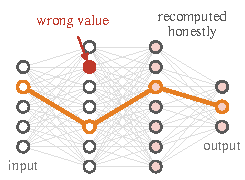
\includegraphics[width=0.47\columnwidth]{figures/overview_attack.pdf}}\hfill
  \subfloat[Defence: caught except with probability $2^{-\lambda}$]{%
    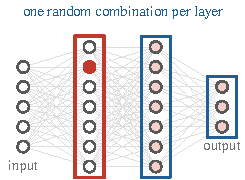
\includegraphics[width=0.47\columnwidth]{figures/overview_defence.pdf}}
  \caption{One tampered neuron whose later layers are recomputed honestly slips past a random path
  (a) but not past a check of every layer (b)}
  \label{fig:overview}
\end{figure}

\para{The attack.} A provider that wants to change an answer does not need a different model. It
runs the committed model, overwrites the value of a single neuron, and recomputes every later
layer honestly with the true weights. The resulting trace is inconsistent at exactly one site,
which a random path visits with probability $1/N$ (Figure~\ref{fig:overview}). On an MNIST network the tampered answer is
accepted with probability 99.6--99.8\%, and on the real OPT-6.7B, editing one feed-forward neuron
changes the next token for 40 of 40 prompts. Applied only to inputs that carry a trigger, the edit
is a backdoor in the serving code: the committed weights stay clean, and clean queries are
answered bit for bit as before. The attack also refutes a claim made for binary classifiers, for
which Anchuri et al.\ state that their analysis extends to full soundness. On a dog-vs-cat
ResNet-18, one changed penultimate neuron flips every test query and passes a path with
probability $511/512$. More paths do not help at a useful cost: catching the attack on Llama-2-7B
with probability $1-2^{-40}$ takes about 305{,}000 paths, which open about 13.7\,GB for a 64-token
prompt.

\para{A dichotomy for spot-checking.} The attack is an instance of a general limit. Because the
provider recomputes everything after the edit, the forged trace is the \emph{honest} trace of a
model that differs from the committed one in a single weight row. Suppose a verifier reads the
weights through a commitment in which each symbol it can query depends on at most $d$ rows, and
makes $q$ queries to a layer in expectation. We show that, when the other rows carry no information
about where the edit is, the verifier rejects the forgery at most as often as it could guess the
edited site in $qd$ tries (Theorem~\ref{thm:guess}). This holds for adaptive,
value-aware verifiers that read the whole claimed trace. In the worst case no verifier beats
uniform sampling: for every such verifier there is a ReLU network with a hidden layer of width $N$
and a single-neuron forgery, with every value in its natural range, that is accepted with
probability at least $1-qd/N$. Soundness $1-\varepsilon$ therefore requires
$qd \ge (1-\varepsilon)N$. Conversely, symbols that mix every row of a layer, such as random
linear combinations of its rows or the columns of a Reed--Solomon encoding of its weights, reach
$2^{-\lambda}$ with $O(\lambda)$ queries per layer, so the threshold is $\Theta(N)$ up to a factor
$O(\lambda)$ (Theorem~\ref{thm:dich}). That spot checks of an unencoded object catch a one-symbol
change only with probability about $q/N$ is
folklore~\cite{juels2007por,ergun2000spotcheckers,bghsv2006robust}. Our contribution is the
reduction that extends this limit to verifiers that read the whole trace, and its consequence: the
object that must be encoded is the model, not the trace. We apply the theorem to published schemes
under their own parameters (Table~\ref{tab:sok}). Most state probabilistic guarantees that their
sampling meets; for example, one audit of SLP's 70B configuration accepts an edited chunk with
probability 98.14\%. We do not call these schemes broken. Two claims exceed what the sampling
gives: the path protocol's full soundness for binary classifiers, and the negligible soundness
that TensorCommitments sets as its goal while choosing the checked layers by a rule that depends
only on the weights, so that an edit in a layer it does not choose always passes. We disclosed
these findings to the authors of the schemes before submission \todo{true only once the notices
scheduled for 15--19 Oct are sent; otherwise delete this sentence; summarise the replies in the
disclosure paragraph of Section~\ref{sec:sok}}.

\para{A defence that checks everything.} Since no verifier has a better worst-case guarantee than
uniform sampling, ours checks every weight operation of the model. The committed model is an int8
network whose results are bit-identical on the provider's GPU and on the client. With the output,
the provider sends the result of every weight operation. The verifier recomputes every operation
without weights, attention included, from these values, and checks each weight operation with a few
random linear combinations of its output rows (Freivalds' algorithm~\cite{freivalds1977}). A client
that does not hold the weights checks each combination against a Reed--Solomon-encoded,
Merkle-committed copy of them, in the style of Ligero~\cite{ligero}, and stores only a 32-byte root
per weight matrix. A tampered value anywhere in the network is then caught except with probability
$2^{-\lambda}$, and the protocol needs only a hash function and a linear code: no SNARK, no trusted
hardware and no trusted setup.

This design leaves four gaps, which we close. First, its soundness theorem assumes an
honestly computed commitment, and this assumption carries weight. A commitment that binds one model
on half of the encoded positions and a modified model on the other half lets the modified model
pass with probability about $2^{-t}$ per query for $t$ opened columns, which is $2^{-35}$ for the
smallest tree of Llama-2-7B. A one-time public setup proof, a proximity test that any client checks once,
removes the assumption (Section~\ref{sec:setup-proof}); for open-weight models anyone can instead
recompute the commitment from the checkpoint. Second, the Fiat--Shamir transcript binds the whole
computation, including every constant of the operations without weights, which avoids the weak
Fiat--Shamir pattern~\cite{bernhard2012pitfalls,dao2023weakfs}. Third, a generated response is
proved as one prefill. The verifier checks each generated token against the claimed logits before
it, either as the greedy choice or as the choice of an exact integer Gumbel-max sampler keyed by a
seed that the client picks, and neither rule adds a soundness term (Section~\ref{sec:gen}).
Fourth, we shrink the proof, which at long prompts consists mostly of the 32-bit results of the
weight operations. In V1 the provider sends instead the int8 value that the next operation reads,
and proves with a logUp-GKR~\cite{haboeck2022logup,papini2023logupgkr} that every hidden result
lies in the requantisation window of the value sent. The verifier knows each operation's input, so
these window conditions are linear in the committed weights, and the GKR's final claim reduces to
the existing folded rows and column check. V1 adds no commitment (Section~\ref{sec:v1}).

\para{Costs.} Beyond the forward pass, the prover's work without V1 grows with the model but not with
the input, and the prover is the protocol's strongest axis. Computing its column openings and folds with exact int8
tensor-core products instead of float64 makes it 3.7--4.3$\times$ faster on Llama-2 blocks on an
RTX~2080~Ti, and it proves a 256-token GPT-2 response to a 64-token prompt in 0.29\,s. On matched
models it is 46--32{,}000$\times$ faster than published zkSNARK provers \todo{L40S: final range; the
current one is from the pre-improvement L40S run}. The main cost is the proof. It carries the
results of every weight operation and so grows with the prompt: 325\,MB for a 64-token Llama-2-7B
query and 6.6\,GB at 2{,}048 tokens \todo{L40S}, against 183\,kB for zkLLM. V1 makes it
2.0--2.3$\times$ smaller at 2{,}048 tokens (the full OPT-1.3B: 2.07 to 0.96\,GB), at the price of
a GKR in the prover whose work grows with the number of results (OPT-125M at 2{,}048 tokens: 0.50
to 4.85\,s on the RTX~2080~Ti) and a CPU verifier that is 1.6--1.9$\times$ slower at that length \todo{L40S}. The verifier recomputes attention, so its cost
grows with the square of the prompt length. With eight CPU threads, a client that holds the weights
verifies a 64-token Llama-2-7B query in about 1.5\,s, against 3.5\,s for re-executing the model in
fp32, but at 2{,}048 tokens the two take about the same time, about 85\,s \todo{L40S/EPYC:
re-measure with the native attention kernel}. Our GPU claim decoder and fused exact attention kernel
make the streaming GPU verifier 2.7$\times$ faster on OPT-1.3B at that length \todo{L40S, full
models}. The protocol is not zero-knowledge: the
claims of $\lceil k/T\rceil$ queries of $T$ tokens reveal a weight matrix with rows of length $k$.
It therefore targets open-weight models served by an untrusted provider, the setting of
CommitLLM~\cite{commitllm2026} and of Gupta et al.~\cite{gupta2026private}. Finally, the provider
must serve the integer model. Moving SmoothQuant's per-channel scales~\cite{xiao2023smoothquant}
into the gains of the integer LayerNorm brings its WikiText-2 perplexity within a factor of 1.03 of
fp32 on OPT-125M and OPT-1.3B, from 1.17 and 1.11, without changing any operation that the
protocol checks \todo{OPT-6.7B and Qwen3-4B with smoothing}.

\para{Contributions.} We make the following contributions.
\begin{itemize}
  \item \emph{An attack on spot-checking proofs of inference} (Section~\ref{sec:attack}): a
  single-site edit followed by honest recomputation, measured on image classifiers and on the real
  OPT-6.7B. It passes the path protocol of~\cite{anchuri2026verifiable} with probability $1-1/N$
  per path and refutes its full-soundness claim for binary classifiers.
  \item \emph{A dichotomy theorem and a systematisation} (Section~\ref{sec:sampling},
  Table~\ref{tab:sok}): against honest recomputation, a verifier that reads the weights through a
  commitment of locality $d$ needs $qd \ge (1-\varepsilon)N$ per layer, which mixing commitments
  meet with $O(\lambda)$ queries. We apply it to nine published inference-verification schemes.
  \item \emph{A fully sound Freivalds-based protocol that needs only a hash function and a linear
  code}
  (Sections~\ref{sec:defence}--\ref{sec:v1}), sound against an untrusted committer, with a
  Fiat--Shamir transcript bound to the whole computation, greedy and sampled generation, and V1,
  which halves the proof at long prompts.
  \item \emph{An evaluation} (Section~\ref{sec:results}) of the attack and the defence on image
  classifiers and language models up to 13B parameters, with re-execution baselines, the quality
  of the integer models, and comparisons with published systems \todo{L40S}.
\end{itemize}

% =====================================================================================
\section{Related Work}
\label{sec:related}

\para{zkSNARK proofs of inference.} A long line of work compiles neural networks into succinct
proofs. For CNNs these include sum-check and GKR provers~\cite{gkr} such as zkCNN~\cite{zkcnn},
zkPyTorch~\cite{zkpytorch} and VerfCNN~\cite{verfcnn}, and pairing- or Plonk-based systems such as
vCNN~\cite{vcnn}, ZEN~\cite{zen}, ZENO~\cite{zeno}, ZKML~\cite{zkml}, EZKL~\cite{ezkl} and
Bionetta~\cite{bionetta}; Mystique~\cite{mystique} is an interactive, VOLE-based alternative. For
language models they include zkLLM~\cite{zkllm}, zkGPT~\cite{zkgpt}, DeepProve~\cite{deepprove},
ZKTorch~\cite{zktorch}, Jolt Atlas~\cite{joltatlas} and the full mode of NanoZK~\cite{nanozk}. They
give computational soundness with proofs of under a kilobyte to tens of megabytes, and many of them
hide the weights. Their provers are far slower than inference. zkLLM takes 620\,s on an A100 for a
2{,}048-token Llama-2-7B prompt, with a 183\,kB proof~\cite{zkllm}; ZKTorch takes 44\,min for one
Llama-2-7B token~\cite{zktorch}; DeepProve takes 34\,s for a 64-token GPT-2 prompt on a 16-core
CPU~\cite{deepprove}. DeepProve and zkAgent~\cite{zkagent} prove a generated sequence in one pass
over the prompt and the output, which is also how we prove generation. These systems prove
non-linear operations with lookup arguments, such as zkLLM's tlookup and the
logUp-GKR~\cite{papini2023logupgkr} that DeepProve uses. V1 borrows this
machinery for one narrow purpose, to show that hidden results lie in their requantisation windows.
The weight products still go through Freivalds' check against the existing commitment, and no
activation is committed. Hollow-LLM~\cite{hollowllm} observes that a valid proof over committed
private weights does not establish that the provider performed the computation of a model of the
declared size, since weights with a degenerate algebraic structure keep the declared shapes but are
cheap to evaluate. Our protocol shares this limitation for private weights; for open weights the
commitment is recomputed from the checkpoint. Our protocol gives up the zkSNARKs' small proofs and weight privacy in exchange for a prover that
is orders of magnitude faster.

\para{Spot-checking and sampling.} Anchuri et al.~\cite{anchuri2026verifiable} spot-check random
paths through a committed trace and prove other-model soundness through trace separation.
SLP~\cite{slp} commits every chunk boundary and proves a random subset of chunks with a SNARK.
CommitLLM's routine audit~\cite{commitllm2026} opens 10 of 80 layers at one token of an audited
response. TensorCommitments~\cite{tensorcommitments} and NanoZK's audit mode~\cite{nanozk} check a
subset of layers, SPEX~\cite{spex} re-executes with a fixed probability, and
IMMACULATE~\cite{immaculate} audits a fraction of requests. TOPLOC~\cite{toploc} and
SVIP~\cite{svip} fingerprint hidden states and target model, prompt or precision substitution.
Verde~\cite{verde}, opML~\cite{opml} and TAO~\cite{tao} are optimistic: an answer stands unless a
party that re-runs the model disputes it, so they rely on an honest party that re-runs every query.
Table~\ref{tab:sok} places these designs under our theorem. SLP and CommitLLM themselves describe
the edit-then-recompute strategy~\cite{slp,commitllm2026}, and the calculation behind it is
classical. It underlies proofs of retrievability and of data
possession~\cite{juels2007por,ateniese2007pdp}, it is why spot-checkers certify only
closeness~\cite{ergun2000spotcheckers}, and it is why PCPs of proximity guarantee only that their
input is close to the language while holographic proofs encode their
input~\cite{bghsv2006robust,bfls1991,chiesa2020fractal}. Our theorem turns this calculation into a
bound for adaptive, value-aware verifiers that read the whole trace; its tight case is the optimal
search for a hidden object~\cite{kadane1971}. Proof-of-Learning~\cite{jia2021pol}, which checks the
largest weight updates of a training run, is a precedent for value-dependent sampling being
gamed~\cite{zhang2022pol,fang2023pol}.

\para{Trusted hardware.} Slalom~\cite{slalom} checks the linear layers of a GPU computation from
inside an SGX enclave with Freivalds' algorithm, optionally with a precomputed secret challenge.
TwinShield~\cite{twinshield} and VeriAttn~\cite{veriattn} extend enclave-based checking to
attention, and VeriAttn accepts results within a tolerance. These designs are fast, but their
guarantee rests on the enclave and its vendor. Our protocol needs no trusted hardware, and its exact
integer semantics leaves no tolerance in which to hide a change.

\para{Freivalds-based checks.} SafetyNets~\cite{safetynets} uses interactive proofs
for networks with quadratic activations, and ZKML~\cite{zkml} uses Freivalds' check for linear layers
inside a SNARK. Maverick~\cite{maverick} checks every linear layer of a language model with sparse
Freivalds checks against a code-encoded copy of the weights that the client stores. Gupta et
al.~\cite{gupta2026private} run Freivalds' check in the exponent of a group, against verification
data that the model owner generates with secret randomness, for a client that outsources inference
to two non-colluding servers. CommitLLM~\cite{commitllm2026} checks int8 language models with secret
Freivalds vectors precomputed from the weights, at 12--14\% serving overhead, and audits attention
without verifying it. LAMP~\cite{lamp} lets a verifier that holds only a commitment check one matrix
product, with Freivalds' check and Reed--Solomon proximity testing inside a Groth16 SNARK. Our column
check is that of the Ligero and Brakedown commitments~\cite{ligero,brakedown}, and our setup proof
is a one-time proximity test in the style of Ligero. Among zkSNARKs, DeepProve's hash-based
configuration commits with BaseFold~\cite{basefold}.

\para{Where we fit.} We keep the setting of Anchuri et al., a client that holds only a commitment to
the weights, and replace the sampled check, which needs $(1-\varepsilon)N$ paths per layer for
soundness $1-\varepsilon$ (Theorem~\ref{thm:dich}), with a check of every weight operation. Each of
the protocols above that avoids a SNARK needs more than a cryptographic commitment: Slalom an
enclave, Maverick an encoded copy of the weights, CommitLLM a secret derived from them, and Gupta
et al.\ public data that grows with every matrix and is generated with secret randomness. zkSNARKs
that verify against a Merkle root, such as DeepProve with BaseFold, need no trusted setup but prove
far more slowly. To our knowledge, ours is the first Freivalds-based proof of inference that is
fully sound for complete transformers, attention included, whose client needs no enclave, no stored
copy of the weights and no weight-derived secret. It uses no SNARK, only a hash function and a
linear code, and with the setup proof it does not trust the party that computes the commitment.

% =====================================================================================
% sections/attack.tex: the attack section (IEEE S&P 2027 submission, IEEEtran compsoc)
%
% Sources used (paths relative to session 4aa2c028's scratchpad); every number below comes from one
% of them:
%   wt_sp2027/report/main.tex      course paper: Sec. 3.1 (setting, threat model), Sec. 3.2 (path test,
%                                  single-neuron attack), Sec. 3.3 (sampling), Sec. 4.1 (models),
%                                  Sec. 4.2 "Breaking the path protocol" (every measured attack number)
%   sp2027_research/attack_theory/PART1_SP.md  Sec. 1 (theorems and proofs with every fix of
%                                  theorem_check.md), Sec. 2 (table tab:sok and its discussion),
%                                  Sec. 3.3 (stored sampler numbers: defence.json, floor_sampler.json),
%                                  Sec. 4 (ethics and disclosure text)
%   attack_theory/theorem.md, theorem_check.md (model, condition (H), Merkle hiding, tightness,
%                                  novelty framing)
%   attack_theory/sok.md, sok_check.md, sok_formulas_out.json (rows, verdicts, acceptance numbers)
%   attack_theory/disclosure.md    (notice plan, schedule and wording)
%   attack_theory/experiments.md   (status of G3/G4; stored numbers; calibration caveat)
%   wt_sp2027/SP2027_PLAN.md       (G1-G5 status; D4 untrusted commitment)
%   wt_sp2027/docs/improvements/D4_D5_untrusted_commitment.md (setup proof; Prop. prop:amp)
%   wt_sp2027/report/references.bib; extra.bib (keys added by the intro agent and by this section)
% Recomputed with Python on 2026-10-10 and matching the sources: (1-1/N)^s, 99.80% (N=512),
% 61.3% (250 paths), paths for 2^-40 = ceil(40 ln 2 / -ln(1-1/N)): 2,316 (N=84), 14,182 (N=512),
% 305,193 (N=11,008), 454,248 (N=16,384); SLP 1-3/161 = 98.14%, 37/160 audits; CommitLLM 1-10/80,
% and 1-0.05/8 = 99.375% per one-token response (shown as approx. 99.4%).
%
% Labels defined here: sec:attack, sec:threat, sec:path, sec:sampling, thm:guess, sec:dichotomy,
% thm:dich, sec:break, sec:sok, tab:sok. The full statements and proofs are in
% sections/appendix_attack.tex (app:attack, def:H, thm:guess-full, cor:surprise, prop:worst,
% prop:blind, prop:amp, rem:merkle, rem:pointer, rem:scope, tab:aligned).
% Labels used from other sections: sec:related, sec:defence, sec:setup-proof (names as in intro.tex).
% Preamble needs: amsmath, amssymb, booktabs, amsthm; fallbacks for the environments follow.
% Compile-checked on 2026-10-10 in a stub IEEEtran (conference,compsoc) document with tectonic:
% no undefined references or citations, no overfull boxes.
% =====================================================================================

\providecommand{\para}[1]{\par\noindent\textbf{#1}\quad}
\providecommand{\todo}[1]{\textbf{[TODO: #1]}}
\providecommand{\toprule}{\hline}
\providecommand{\midrule}{\hline}
\providecommand{\bottomrule}{\hline}
\makeatletter
\@ifundefined{theorem}{\newtheorem{theorem}{Theorem}}{}
\@ifundefined{lemma}{\newtheorem{lemma}{Lemma}}{}
\@ifundefined{corollary}{\newtheorem{corollary}{Corollary}}{}
\@ifundefined{proposition}{\newtheorem{proposition}{Proposition}}{}
\@ifundefined{definition}{\newtheorem{definition}{Definition}}{}
\@ifundefined{remark}{\newtheorem{remark}{Remark}}{}
\@ifundefined{proof}{\newenvironment{proof}[1][Proof]{\par\noindent\textit{#1.}\ }{\hfill$\square$\par\smallskip}}{}
\makeatother

\section{Attacking Spot-Checking Proofs of Inference}
\label{sec:attack}

This section shows that a proof of inference that checks a sample of an unencoded execution trace
is not fully sound, and that no sampling rule can make it so.

% -------------------------------------------------------------------------------------
\subsection{Setting and Threat Model}
\label{sec:threat}

A model $M$ has a public architecture, and the client may not hold its weights. The provider acts
as the prover and the client as the verifier. Before any query the client obtains a commitment
$C_M$ to the weights. For each query $x$ the provider returns a claimed output $y$ and a proof. We
require \emph{completeness}, meaning that honest answers are always accepted, and \emph{full
soundness} with error $\varepsilon$: any $y\neq M(x)$ is accepted with probability at most
$\varepsilon$. Anchuri et al.~\cite{anchuri2026verifiable} prove only \emph{other-model
soundness}, against a provider that honestly runs a different model.

\para{Spot-checking.} The provider commits to the execution trace, and the verifier checks a few of
its \emph{sites}. A site is a unit of the computation that can be checked locally against committed
data, such as a neuron and its incoming weights in the path protocol, a chunk of layers in
SLP~\cite{slp}, or a (layer, token) cell in CommitLLM's routine audit~\cite{commitllm2026}. For each
sampled site the verifier opens its inputs, its value and the weights it uses, and checks that the
value follows from them. The trace carries no error-correcting encoding, so a change to one value is
visible at one site only.

\para{Adversary.} The provider controls its serving code and may deviate from the protocol
arbitrarily. It keeps the committed weights. It knows the verifier's sampling rule, including rules
that adapt to the claimed values, but not the verifier's coins. It chooses which queries to tamper
with, and on those queries it returns a wrong answer (untargeted) or an answer of its choice
(targeted). As in~\cite{anchuri2026verifiable}, $C_M$ is computed honestly; the attack does not
change it.

% -------------------------------------------------------------------------------------
\subsection{The Path Protocol and the Single-Site Edit}
\label{sec:path}

In the protocol of Anchuri et al.\ (RandPathTest), the prover commits to every activation $a_j$ of
the forward pass with a Merkle tree~\cite{merkle1987}. The verifier chooses a random output neuron
and walks back to the input, moving to a random parent at each layer. At every node $j$ on the path
it opens the parents' activations and the weights $w_{ij}$ from $C_M$, and checks
$a_j=\phi\big(\sum_{i\in G_j}w_{ij}a_i\big)$ up to a floating-point tolerance, where $G_j$ is the
set of parents of $j$ and $\phi$ the activation. A path opens one weight row per layer, so proofs
stay small. Anchuri et al.\ note that one path catches a single changed node with probability at
most $1/N$ in a layer of width $N$. As mitigations they suggest more paths, or sampling where it
matters instead of uniformly.

\para{The single-site edit.} Our adversary runs the correct model on $x$, picks one neuron $u$, and
replaces $a_u$ by a value that makes the output wrong, or equal to a class of its choice. To find
$u$, it ranks neurons by the gradient of the decision margin and bisects for the smallest edit that
changes the output. It then recomputes all later layers \emph{with the true weights}, so $u$ is the
only node whose check fails. A path visits $u$ with probability $1/N$ in a dense layer, and one of
$s$ paths does so with probability $1-(1-1/N)^s$. Applied only to inputs that carry a trigger, the
edit is a backdoor~\cite{gu2019badnets} in the serving code: the committed weights stay clean, and
clean queries are answered bit for bit as before.

\para{Repeated queries.} Anchuri et al.\ observe that repeated queries amplify detection. This holds
against a provider that cheats on every query. Ours tampers only with the $k$ queries it cares
about, and is caught on any of them with probability at most $1-(1-1/N)^k\le k/N$.

% -------------------------------------------------------------------------------------
\subsection{Why Sampling Cannot Fix It}
\label{sec:sampling}

We now show that neither mitigation helps against an adversary who knows the rule, even for an
adaptive verifier that reads the entire claimed trace and chooses where to look from its values.

\para{Model.} Fix one weight layer of width $N$, the \emph{target layer}. Give the verifier for free
the query $x$, all other layers, public side information $Z$ (such as each neuron's natural range)
and the entire claimed trace $\tau'$; we call $P=(x,Z,\tau')$ its \emph{view}. Row $\theta_i$ holds
the incoming weights and the bias of neuron $i$, whose value on $x$ is $h_i=f_i(\theta_i)$. The
verifier learns $\theta$ only through a commitment oracle. A query $\sigma$ returns a symbol that
depends on the rows in its \emph{support} $S_\sigma$, and the oracle has \emph{locality} $d$ if
$|S_\sigma|\le d$ for every query. A row-wise commitment, as in the path protocol, has $d=1$ as long
as its openings reveal nothing about unopened rows (Remark~\ref{rem:merkle}). A column of the
Reed--Solomon commitment of Section~\ref{sec:defence}, or a random combination $\chi^{\top}\!A$ of
the layer's rows, has support $[N]$. The verifier \emph{touches} neuron $u$ if some query has
$u\in S_\sigma$. It chooses each query from $P$, its coins and the earlier answers, and it must
accept the honest trace of every \emph{admissible} instance, that is, every instance consistent
with $Z$. In the target layer, $s$ paths make $s$ queries of locality~$1$.

\para{Honest recomputation hides the edit.} The edited trace is the \emph{honest} trace of an
admissible model that differs from the true one in row $u$ alone. For a ReLU neuron with a bias,
that row has zero weights and bias $v$, or $-1$ if $v=0$. We call such a forgery
\emph{explainable}. Without recomputation every child of $u$ would be inconsistent, and an adaptive
verifier could follow the inconsistencies back to $u$.

\begin{theorem}[spot-checking is guessing the location]
\label{thm:guess}
Let $J$ be the neuron that the adversary edits, and suppose that the rows other than $J$ carry no
information about $J$ beyond the view (condition~(H) of Definition~\ref{def:H}; it holds, for
example, when the rows are independent and the adversary chooses $J$ from the values $h$ alone).
Let $V$ make, in expectation, at most $q$ queries that meet the target layer. Then $V$ rejects an
explainable single-site forgery with probability at most
\[
  G_{qd}(J\mid P) \;=\; \mathbb E_{p}\Big[\max_{|S|\le qd}\Pr[J\in S\mid P=p]\Big],
\]
the probability of guessing $J$ in $qd$ tries from the view alone. For $d=1$ the bound is attained
by a verifier that knows the adversary's strategy and opens the $q$ neurons most likely to have
been edited.
\end{theorem}

\noindent Opening rows therefore only confirms that they are clean, and adaptivity adds nothing
beyond a good guess. This is the classical result on searching for a hidden
object~\cite{chew1967,kadane1971}, with a clean opened row in the role of an empty box. What is
specific to proofs of inference is that honest recomputation makes it apply to verifiers that read
the whole trace. Condition~(H) is needed: if one row stores the location of the critical neuron,
two adaptive queries catch the edit with certainty (Remark~\ref{rem:pointer}). Trained networks
have correlated rows, so for them we rely on the worst case of Section~\ref{sec:dichotomy}.

\para{What reading the values buys.} With independent rows, the posterior on the edited neuron is
proportional to the adversary's propensity to choose it, divided by the prior probability of the
value written there (Corollary~\ref{cor:surprise}). A value-aware sampler therefore gains on edits
that write improbable values. It gains nothing on edits that write common ones, provided the
adversary's choice of neuron is itself spread out. Our measurements are consistent with this but do
not test it directly. The contribution-weighted sampler detects 9.2\% of the best single-neuron
edits and none of the zeroing edits; for the latter the reason is mechanical, since it never visits
a neuron whose claimed activation is zero (Section~\ref{sec:break}). \todo{G1e tamper locator:
top-$q$ hit rate of a locator that ranks sites from the forged trace alone, i.e.\ the empirical
$G_q$ of our greedy attack and of a randomised one, MNIST MLP, $q\in\{1,\dots,64\}$}

% -------------------------------------------------------------------------------------
\subsection{A Dichotomy}
\label{sec:dichotomy}

Soundness quantifies over every network, and on a suitable network (H) holds by construction. This
gives one half of a dichotomy. Our defence gives the other half.

\begin{theorem}[dichotomy]
\label{thm:dich}
Consider verifiers that read each layer's weights through a commitment of locality $d$ that
reveals nothing about unopened rows, and let $q$ be the expected number of queries that meet a
layer of width $N$.
(a)~\emph{Spot-checking.} For every such verifier there is a ReLU network with a hidden layer of
width $N$, and a single-site forgery with every value in its natural range, that the verifier
accepts with probability at least $1-qd/N$, even if it knows the later weights, every neuron's
natural range and the natural distribution of each neuron of that layer. In particular, a verifier that spot-checks $q$ of the $N$ sites of
an unencoded trace ($d=1$) accepts with probability at least $1-q/N$, whatever its sampler, and
soundness error at most $\varepsilon$ on every such network requires $qd\ge(1-\varepsilon)N$.
(b)~\emph{Mixing.} If each query mixes all rows ($d=N$), as the folded rows and code columns of
Section~\ref{sec:defence} do, then under the conditions of Proposition~\ref{prop:amp},
$O(\lambda+\log L)$ queries per layer give soundness error $2^{-\lambda}$ for a network of $L$
weight layers. For $L\le2^{\lambda}$ this is $O(\lambda)$, so $qd=O(\lambda)N$ suffices.
\end{theorem}

\begin{proof}[Proof idea]
For~(a), hidden neuron $i$ copies input bit $\sigma(i)$ for a uniformly random permutation
$\sigma$. Natural inputs have at most one zero, and the output is $1$ exactly when every hidden
neuron is $1$. On a query whose zero is at $\zeta$, the adversary sets the neuron that copies $\zeta$ to
$1$, which flips the output and stays in the range $\{0,1\}$. The forged trace, the later weights,
the ranges and the hidden marginals do not depend on $\sigma$, so the edited neuron is uniform
given the view, and Theorem~\ref{thm:guess} bounds detection by $qd/N$. Random weights on inputs
that are always zero keep each opening from revealing other rows. Part~(b) restricts the soundness
argument of our defence to one layer: a wrong claim survives a random fold with probability $1/p$
and an opened column with probability at most $(k-1)/n$. Appendix~\ref{app:attack} gives the full
proofs (Propositions~\ref{prop:worst} and~\ref{prop:amp}).
\end{proof}

\para{What the dichotomy means.} Opening $s$ distinct neurons uniformly reaches $s/N$ on every
dense network, so in the worst case nothing beats uniform sampling. Reaching $2^{-40}$ then takes
about $27.7N$ paths per query, which is the cost the path protocol was designed to avoid. The two
regimes differ by a factor $O(\lambda)$ in $qd$, and in both the verifier touches every row; mixing
lowers the cost of each touched row from a full row of weights to $O(\lambda)$ field elements.
Part~(a) is the one-sided randomised query complexity of $\mathrm{OR}_N$ placed inside a network,
and the spot-check calculation behind it is folklore (Section~\ref{sec:related}). Our contribution
is the reduction that extends it to adaptive, value-aware verifiers that read the whole trace.
Because the trace is then free to read, the object that must be encoded or folded is the model, not
the trace. Our defence encodes only the model, which is why its proof still grows with the trace.

% -------------------------------------------------------------------------------------
\subsection{Measured Attacks}
\label{sec:break}

We implemented the path protocol and attacked an MNIST MLP (784--512--256--10), LeNet-5, VGG-11,
VGG-16 and ResNet-18 on CIFAR-10, a 224$\times$224 dog-vs-cat ResNet-18 that stands in for the
unreleased model of~\cite{anchuri2026verifiable}, and the real OPT-6.7B. We compute the probability
of passing one path exactly, by dynamic programming over the paths.

\para{Reproduction.} Our implementation behaves as Anchuri et al.\ describe. On MNIST versions of
four of their substitute-model settings, honest provers passed all 3{,}000 runs of each, and
substitute models were caught in 99.8--100\% of runs, including an 8-bit quantised copy that agrees
with $M$ on all 150 evaluated queries. Without the $10^{-4}$ tolerance, an honest prover passes only
21--37\% of runs, because a layer-wide matrix product and a single-neuron dot product round
differently.

\para{MNIST.} The forgeries that Anchuri et al.\ consider (their substitute model, Appendices~E
and~F and Section~7.2 of~\cite{anchuri2026verifiable}) corrupt hundreds of the MLP's 778 trace nodes
and are always caught. Ours leave 1--14 inconsistent nodes. One tampered neuron passes with the
predicted probability $1-1/N$ (99.6--99.8\%), and still passes 250 paths 61\% of the time. A
backdoor triggered by a $3{\times}3$ bright patch returns the honest output on every clean query and
succeeds on every triggered query not already in the target class. It passed 99.96\% of 2{,}300
end-to-end runs, within sampling error of the predicted 99.8\%. Keeping each tampered value below
its neuron's 95th percentile takes about five neurons and still passes 99\% of the time under
uniform sampling.\footnote{These percentiles were computed on test queries that include the
attacked ones. \todo{G3: repeat with ranges calibrated on the training split; report separately
the plans whose edited values, and whose every claimed value, are in range}}

\para{Other samplers.} Against an adversary who knows the rule, uniform sampling detects 0.20\% of
attacks, a static importance score (outgoing weight magnitude) 0.11\% and gradient saliency
0.016\%. The contribution-weighted sampler, which steps to parent $i$ with probability proportional
to $|w_{ij}a_i|$, detects 9.2\% of the best single-neuron edits. Zeroing about 14 of the 512
neurons instead, whose most common value is zero (65\% of inputs), flips the prediction and passed
2{,}000 of 2{,}000 end-to-end runs. A floor $\delta$, sampling by $|w_{ij}|(|a_i|+\delta)$, reaches
2\% at $\delta=1$ (10$\times$ uniform); other floors give 0.9--6$\times$. Each figure is the
detection of the best attack we found, and so an upper bound on worst-case detection. \todo{G3
adaptive game: per-path detection of the best value-aware sampler and of the LP-optimal sampler
mixture against range-respecting edits with held-out ranges, MNIST MLP and CNN heads, with the
paths needed for $2^{-40}$}

\para{Larger models.} On every CNN and every test query, changing one penultimate neuron flips the
prediction. One path catches it with probability 1/84 (LeNet-5) to 1/512 (VGG, ResNet), and a
change to the least-visited neuron with probability as low as 1/28 million. This includes the
dog-vs-cat ResNet-18, a binary classifier, for which Anchuri et al.\ state that their analysis
extends to full soundness. Reaching $2^{-40}$ takes 2{,}316--14{,}182 paths, which open the whole
model and trace. In the FFN layers of Llama-2-7B (width 11{,}008), $2^{-40}$ needs at least
305{,}193 paths, about 13.7\,GB of openings with the fp16 weights of~\cite{anchuri2026verifiable}
at 64 tokens.

\para{A real LLM.} On the real OPT-6.7B (fp16), the same search over FFN neurons of layers 8, 16, 24
and 31 at the last position changed the next token with one neuron for all 40 prompts. A
fixed-target backdoor is more constrained. Because of the final LayerNorm, a last-layer neuron can
force only its \emph{saturation token}, so the 16{,}384 neurons of that layer reach 6{,}187 of the
50{,}272 tokens. The backdoor succeeds for ``\texttt{back}'' (40/40 triggered prompts, clean
prompts unchanged) and fails for ``\texttt{hacked}'' (0/40). Its values exceed the neurons' natural
range, which the path protocol does not check, and $2^{-40}$ needs at least 454{,}248 paths.
\todo{L40S: next-token attack on OPT-6.7B with values kept within ranges calibrated on WikiText-2
training text (plan item G3.5), if run} Under the path protocol, detection depends only on how
many sites are edited, so Table~\ref{tab:aligned} gives the paths needed for $k$ edited neurons in
two instruction-tuned models. We do not develop a method for steering their responses.

% -------------------------------------------------------------------------------------
\subsection{Systematisation of Spot-Checking Schemes}
\label{sec:sok}

\begin{table*}[t]
  \caption{Spot-checking schemes against one changed value followed by honest recomputation,
  under each scheme's own sampling rule and parameters}
  \label{tab:sok}
  \footnotesize
  \setlength{\tabcolsep}{4pt}
  \def\rr{\raggedright}%
  \begin{tabular}{@{}p{2.3cm}p{3.1cm}p{4.6cm}p{3.8cm}p{2.0cm}@{}}
    \toprule
    \rr Scheme & \rr What is checked & \rr Edit accepted with & \rr Stated guarantee &
      \rr Claim beyond sampling? \tabularnewline
    \midrule
    \rr Path protocol~\cite{anchuri2026verifiable} &
      \rr one output-to-input path; every visited neuron &
      \rr $(1-1/N)^s$: 99.80\% ($N{=}512$, $s{=}1$), 61.3\% ($s{=}250$); $2^{-40}$ needs 14{,}182
      paths (ResNet-18$^a$), and at least 305{,}193 and 454{,}248 (Llama-2-7B, OPT-6.7B$^a$) &
      \rr other-model soundness (proved); full soundness said to extend to binary classifiers;
      $1/N$ limit noted &
      \rr yes, for binary classifiers$^b$ \tabularnewline
    \rr SLP~\cite{slp} &
      \rr 3 of 161 non-anchor chunks (70B) &
      \rr 98.14\% per audit; a persistent edit needs 37 / 160 audits for 50\% / 95\% detection;
      88.9\% for TinyLlama (5 of 45) &
      \rr covers proven chunks only (3/161 stated) &
      \rr no \tabularnewline
    \rr CommitLLM, routine audit~\cite{commitllm2026} &
      \rr 1--5\% of responses; one token; 10 of 80 layers (Llama-70B) &
      \rr 87.5\% when the token is opened; $\approx$99.4\% per one-token response at a 5\% audit
      rate; an edited attention output passes every tier (authors' own finding) &
      \rr exact for opened matrices; statistical coverage; attention audited, not verified &
      \rr no \tabularnewline
    \rr Tensor\-Commitments \cite{tensorcommitments} &
      \rr layer intervals chosen deterministically from the weights &
      \rr $1$ for an edit outside the chosen intervals; a random choice of the same size would give
      $1-|S|/L$ &
      \rr soundness $\mathrm{negl}(\lambda)$ against any PPT prover, stated as the goal &
      \rr yes$^c$ \tabularnewline
    \rr NanoZK~\cite{nanozk} &
      \rr full mode: every layer; audit mode: a budget $S$ of layers &
      \rr full: $\le 3\cdot10^{-37}$; audit mode with a uniform 50\% budget: 50\% &
      \rr audit mode presented as an efficiency tool, not a security claim &
      \rr no \tabularnewline
    \rr SPEX~\cite{spex} &
      \rr full re-execution with probability $\delta$ &
      \rr $1-\delta$ per request &
      \rr confidence $\delta$; state sampling ``cannot prevent an adversarial solver'' &
      \rr no \tabularnewline
    \rr IMMACULATE \cite{immaculate} &
      \rr a fraction of requests; verified logit statistics &
      \rr a flipped step adds $1/T$ to the flagged fraction$^d$ &
      \rr model substitution, quantisation, overbilling &
      \rr no (outside claim) \tabularnewline
    \rr TOPLOC~\cite{toploc}, SVIP~\cite{svip} &
      \rr hidden-state fingerprints &
      \rr no edit needed: forged tokens with honestly recomputed fingerprints pass (100\%;
      $\ge$95\%) &
      \rr model, prompt or precision substitution; token choice out of scope &
      \rr no (outside claim) \tabularnewline
    \rr Proof-of-Learning~\cite{jia2021pol} &
      \rr the $Q$ largest updates per epoch (value-aware) &
      \rr 100\% for a ``blindfolded'' update~\cite{fang2023pol} &
      \rr probabilistic &
      \rr broken before~\cite{zhang2022pol,fang2023pol} \tabularnewline
    \bottomrule
  \end{tabular}

  \smallskip
  {\footnotesize Acceptance follows from each scheme's own formulas and parameters; no deployed
  system was tested. $^a$Our models: the dog-vs-cat ResNet-18 that stands in for the unreleased
  model of~\cite{anchuri2026verifiable}, and the real OPT-6.7B; Llama-2-7B uses its FFN width
  11{,}008. $^b$The authors state that their other-model analysis ``trivially extends to full
  soundness'' for binary-output models, while also noting the $1/N$ limit for one changed node;
  their other-model theorem is unaffected, and for LLMs they leave full soundness open. $^c$The
  soundness definition is stated as the problem's goal (no theorem claims it), and the gap comes
  from the predictable, weight-only layer selection, not from the commitment. $^d$Our derivation
  from the flagging rule, for a response of $T$ steps.}
\end{table*}

Table~\ref{tab:sok} applies the bound to published schemes, under each scheme's own sampling rule
and parameters. Every acceptance probability follows from the scheme's own formulas, and we tested
no deployed system. We say that a claim exceeds the sampling only where a stated guarantee is
stronger than what the scheme's own sampling gives.

\para{What the table shows.} An edit followed by honest recomputation is caught exactly when the
sample covers it: $s/N$ for paths, $3/161$ for SLP's 70B configuration, one layer in eight for
CommitLLM's routine audit, $|S|/L$ for NanoZK's audit mode, and never outside the weight-determined
layer selection of TensorCommitments. SLP, CommitLLM, NanoZK and SPEX present their guarantees as
probabilistic, and SLP and CommitLLM describe the edit-then-recompute strategy
themselves~\cite{slp,commitllm2026}. We therefore do not call them broken. By
Proposition~\ref{prop:blind}, no other value-blind sample of the same size would do better against
every placement of the edit. A claim exceeds the sampling in two places. The path protocol's full
soundness for binary classifiers fails on our dog-vs-cat ResNet-18. The negligible soundness error
that TensorCommitments sets as its goal is not met by a deterministic layer selection that the
provider can compute itself. More generally, a selection by value or by a public ranking gives an
adaptive provider a place to hide. A deterministic choice is avoided with certainty, and
value-dependent choices have been evaded by edits that write common values, both by our zeroing
attack and by the blindfolded updates against Proof-of-Learning~\cite{fang2023pol}. TOPLOC and SVIP
target model substitution, and a forged answer with honestly recomputed fingerprints lies outside
what they claim.

\para{Ethics and responsible disclosure.} Our attack targets verification protocols, not deployed services.
Every experiment ran on our own implementations, with public datasets and open-weight models, on
our own hardware. Before submission we wrote to the authors of the path protocol and of
TensorCommitments, CommitLLM, NanoZK, SLP and SPEX \todo{dates the notices were sent; scheduled for
15 Oct 2026 (Anchuri et al., TensorCommitments) and 19 Oct 2026 (CommitLLM, NanoZK, SLP, SPEX);
remove SPEX here and from Table~\ref{tab:sok} if its optional notice is not sent}. For each scheme
we described what we found, under which of its stated parameters, and what we do not claim, and we
offered our draft and code. \todo{summary of the replies; if none: ``We had received no reply by
2~Nov 2026.''} Where a scheme states a probabilistic guarantee, we report the acceptance
probability that follows from its own formulas and do not call it broken. We say that a stated
guarantee is not met only for the path protocol's full-soundness claim for binary classifiers and
for the soundness goal of TensorCommitments. We release no method for steering the responses of
instruction-tuned assistants.

% =====================================================================================
% sections/defence.tex: the defence (Section 4), condensed for the 13-page body (CUT_PLAN.md).
% Sources: the previous draft of this file (course paper Secs. 3.1, 3.4-3.6; plan items A1, A2,
%   D1-D7; code/src/pvi/fullcheck/*). Removed detail and Table tab:setup: sections/ext_defence.tex.
% Labels defined: sec:defence, sec:intmodel, sec:commit, sec:protocol, sec:fs, sec:setup-proof,
%   eq:weightop, eq:freivalds, eq:split, thm:sound, thm:untrusted, fact:ext, fig:protocol.
% Labels used: thm:dich, sec:threat, sec:quality, sec:gen, sec:v1, app:defence, app:semantics,
%   app:sound, app:untrusted. New BibTeX key: fri2018 (fullversion is already in extra.bib).
% =====================================================================================

\providecommand{\F}{\mathbb{F}_p}
\providecommand{\enc}{\mathrm{Enc}}
\providecommand{\T}{\top}
\providecommand{\sC}{\mathsf{C}}
\providecommand{\sK}{\mathsf{K}}
\providecommand{\Kpre}{\mathsf{K}_{\mathrm{pre}}}
\providecommand{\para}[1]{\par\noindent\textbf{#1}\quad}
\providecommand{\todo}[1]{\textbf{[TODO: #1]}}
\providecommand{\qed}{\hfill$\square$}
\makeatletter
\@ifundefined{theorem}{\newtheorem{theorem}{Theorem}}{}
\@ifundefined{fact}{\newtheorem{fact}{Fact}}{}
\makeatother

\section{The Defence: Checking Every Weight Operation}
\label{sec:defence}

Theorem~\ref{thm:dich} leaves one way to reach soundness $2^{-\lambda}$ well below the cost of
re-execution: the verifier must touch every row, through checks that each mix many rows of a weight
matrix. Our defence applies the evaluation protocol of a linear-code polynomial commitment, as in
Ligero and Brakedown~\cite{ligero,brakedown}, to every matrix product: Freivalds'
algorithm~\cite{freivalds1977} tests random combinations of all neurons of each weight operation,
and a client without the weights checks each combination against a Reed--Solomon-encoded,
Merkle-committed copy of them. The commitment's testing phase is amortised into a one-time setup
proof (Section~\ref{sec:setup-proof}). The provider (prover) may deviate arbitrarily. In mode
$\sC$ the client (verifier) holds only a commitment $C_M$ to the weights, as in the path
protocol~\cite{anchuri2026verifiable}; in mode $\sK$ it holds the weights, and in mode $\Kpre$ only secret Freivalds vectors and their
folded rows, precomputed once per model from the weights~\cite{slalom,commitllm2026}. For open
weights anyone can recompute $C_M$ from the checkpoint and the public quantisation recipe
(Section~\ref{sec:threat}) \todo{D6: check that $C_M$ is reproducible}.

% -------------------------------------------------------------------------------------
\subsection{The Exact Integer Model}
\label{sec:intmodel}

Exact checks need exact values: a floating-point tolerance would let a cheating prover hide small
changes. We therefore certify an integer network obtained by integer-only
quantisation~\cite{jacob2018quant}, as related systems do~\cite{safetynets,slalom,zkcnn,zkml,zkllm}.
Soundness refers to this model; Section~\ref{sec:quality} measures its gap to the checkpoint. A
\emph{weight operation} $\ell$ computes
\begin{equation}
  Z_\ell = A_\ell\,[X_\ell;\mathbf 1], \qquad A_\ell=[W_\ell\,|\,b_\ell],
  \label{eq:weightop}
\end{equation}
where $W_\ell$ is an int8 matrix with $N_\ell$ rows, $b_\ell$ an integer bias, $X_\ell$ an int8
matrix with one column for each of its $T_\ell$ positions, and $k_\ell$ the row length of $A_\ell$.
Embeddings are looked up. Every other operation (requantisation, residual addition on 23-bit
integers, integer norms, 256-entry tables for activations and the softmax exponential, 8-bit
attention probabilities) maps integers to integers with public constants
(Appendix~\ref{app:semantics}). The output $y$ is the claim of the last weight operation, for a
language model the next-token logits; Section~\ref{sec:gen} covers generated responses. Integer sums
do not depend on their order, so prover and verifier agree on any hardware: int8 products are at
most $2^{14}$, blocks of $2^{16}$ of them sum exactly in 32-bit integers on tensor cores, and
attention runs in float32 within its exact range. The checks run in the BabyBear field $\F$,
$p=15\cdot2^{27}+1\approx2^{31}$. The verifier rejects every claim with $|z|\ge2^{29}$, and setup
checks that honest claims are smaller ($128\sum_c|w_{ic}|+|b_i|<2^{29}$ for every row $i$ of a
product, $\max_c|w_{ic}|+|b_i|<2^{29}$ for an embedding). A wrong claim and the correct value thus
differ by less than $2^{30}<p$ and remain distinct in $\F$.

% -------------------------------------------------------------------------------------
\subsection{Committing to the Weights}
\label{sec:commit}

At setup, every row of $A_\ell$ is Reed--Solomon encoded~\cite{reedsolomon1960}: the polynomial
whose coefficients are the row is evaluated at the $n\ge k_\ell$ points of a multiplicative subgroup
of $\F$ ($n$ a power of two), giving the rows of $\hat A_\ell$. Encoding is linear, so
$\chi^\T\hat A_\ell=\enc(\chi^\T A_\ell)$, and two distinct codewords agree on at most $k_\ell-1$
positions. A SHA-256 Merkle tree~\cite{merkle1987} binds the columns of $\hat A_\ell$. $C_M$ holds
the roots, 32 bytes per tree, and the public encoding parameters.

\para{Commitment plans.} Matrices whose codewords have equal length can share a tree and a
multiproof. A public rule picks the plan (trees and codeword lengths) that sends the fewest bytes
per query within a cap on the setup size; the plan is part of $C_M$. A layer with many rows, such as
GPT-2's output layer ($N=50{,}257$), encodes the rows of $A_\ell^\T$ instead (the \emph{transposed
layout}), stacking operations that read the same input. An embedding table without a bias is a
Merkle tree over its rows~\cite{commitllm2026}.

% -------------------------------------------------------------------------------------
\subsection{The Protocol}
\label{sec:protocol}

With $y$, the prover sends the \emph{claims} $Z_\ell$ of every weight operation, $y$ among them. All
claims are correct if and only if, for every weight operation $\ell$, (S1)~$X_\ell$ follows from $x$
and the earlier claims through the operations without weights,
(S2)~$Z_\ell=A_\ell[X_\ell;\mathbf 1]$, and (S3)~$A_\ell$ is the committed matrix. In mode $\sC$ a query has three rounds: the claims; the vectors $\chi$ and the folded rows; the column
positions and the opened columns.

\para{(S1): recomputation.} The verifier computes every operation without weights itself, which
chains the checks: no prover can pass one check with one value and feed another into the next.
Attention and the other non-linear operations are not proved; the verifier recomputes them from
checked values.

\para{(S2): Freivalds' check.} After all claims are fixed, the verifier draws a uniform
$\chi_\ell\in\F^{N_\ell\times r}$ and checks
\begin{equation}
  \chi_\ell^\T Z_\ell \;=\; u_\ell\,[X_\ell;\mathbf 1], \qquad u_\ell=\chi_\ell^\T A_\ell,
  \label{eq:freivalds}
\end{equation}
where we call $u_\ell$ the \emph{folded rows}. If $D=Z_\ell-A_\ell[X_\ell;\mathbf 1]$ has
$D_{ij}\neq0$, then for each column $\chi$ of $\chi_\ell$, entry $j$ of $\chi^\T D$ is
$\chi_iD_{ij}+c$ with $c$ independent of $\chi_i$, so it vanishes for one of the $p$ values of
$\chi_i$. A wrong operation thus passes with probability at most $p^{-r}$, however many of its
values are wrong: one tampered neuron is caught as reliably as a wrong layer. Given $u_\ell$, the
check costs $O(r(N_\ell+k_\ell)T_\ell)$ instead of $O(N_\ell k_\ell T_\ell)$.

\para{(S3): the column check.} In mode $\sC$ the prover sends $u_\ell$ (in $\sK$ and $\Kpre$ the
verifier computes it); opening a few entries would miss a single wrong one, as a path misses a
single neuron. The verifier therefore tests $u_\ell$ through the code: it draws $t$ distinct uniform
positions $c$, receives the columns $\hat A_{\ell,c}$ with a Merkle multiproof, and checks the paths
and $\chi_\ell^\T\hat A_{\ell,c}=\enc(u_\ell)_c$. If $u_\ell\neq\chi_\ell^\T A_\ell$, some row of
$\enc(u_\ell)$ and the same row of $\chi_\ell^\T\hat A_\ell$ are distinct codewords, so all $t$
columns fall where they agree with probability at most $\prod_{i<t}(k_\ell-1-i)/(n-i)<(k_\ell/n)^t$.
For a transposed matrix the verifier combines positions with $\chi'\in\F^{T\times r}$ and checks
$\enc(Z\chi')$ against the opened columns combined by $[X;\mathbf 1]\chi'$
(Appendix~\ref{app:sound}). Opened rows of a lookup table are checked against its root.

\para{Modes $\sK$ and $\Kpre$.} In $\sK$ the verifier draws a fresh $\chi_\ell$ for each query, so
the proof is the claims alone. In $\Kpre$ it computes the secret $\chi_\ell$ and $u_\ell$ once per
model. This designated-verifier mode loses soundness if $\chi_\ell$ leaks, and nobody else can check
its proofs.

\para{Costs.} The prover's extra work, $O((r+t)\sum_\ell N_\ell k_\ell)$, does not depend on the
number of positions, and no term of the verifier's work grows with $N_\ell k_\ell T_\ell$. The proof
holds the claims, which grow with $T$, and in mode $\sC$ the folded rows, opened columns and Merkle
paths, which do not; V1 (Section~\ref{sec:v1}) shrinks the claims.

\para{Soundness.} Let $\mathcal J$ hold one committed matrix per row-layout weight operation and per
transposed matrix. Matrix $j$ has message length $k_j$ and codeword length $n_j$, and its tree opens
$t_j$ columns.

\begin{theorem}[soundness]
\label{thm:sound}
Suppose that $C_M$ is computed honestly from the weights of $M$ and that the prover finds no hash
collision. For every input $x$, which the prover may choose, and every prover, the verifier of mode
$\sC$ accepts an output $y\neq M(x)$ with probability at most
\[
  \varepsilon_{\sC}=\sum_{j\in\mathcal J}\Big[\,p^{-r}+\prod_{i<t_j}\frac{k_j-1-i}{n_j-i}\,\Big].
\]
In mode $\sK$ the bound is $\varepsilon_{\sK}=\sum_\ell p^{-r}$, over the weight operations that
are not looked up. In mode $\Kpre$, over $Q$ queries that reuse the secret vectors, the verifier
accepts some $y\neq M(x)$ with probability at most $Q\,\varepsilon_{\sK}$, even if the prover learns
which check failed in every rejected query.
\end{theorem}

\noindent\emph{Proof sketch.} The first wrong weight operation has a correct input, which the
verifier computed from correct claims. With the true $u_\ell$ Freivalds' check fails except with
probability $p^{-r}$, and with another $u_\ell$ the column check fails except with the column term.
In $\Kpre$, until a wrong claim passes, every outcome is a function of the prover's messages, so its
view does not depend on $\chi_\ell$ (Appendix~\ref{app:sound}). \qed

\para{Parameters.} We set $\beta=\lambda+\log_2(2|\mathcal J|)$ and $r=\lceil\beta/\log_2p\rceil$,
and each tree opens the least $t$ that keeps every member's column term below $2^{-\beta}$. Then
$\varepsilon_{\sC}\le2^{-\lambda}$; at $\lambda=128$, $r=5$ (Appendix~\ref{app:defence} lists all
parameters for Llama-2-7B). Each folded row and column mixes all rows of its matrix, so the protocol
attains the upper bound of Theorem~\ref{thm:dich} with $O(\lambda)$ field elements per row instead
of $k_\ell$ weights.

% -------------------------------------------------------------------------------------
\subsection{Non-Interactive Proofs}
\label{sec:fs}

Each challenge is expanded with SHAKE-256~\cite{fips202} from a 256-bit key, which the verifier
draws in interactive runs and which is derived from a transcript under
Fiat--Shamir~\cite{fiatshamir1986}.

\para{The statement binds the computation.} Challenges that do not depend on the whole statement
make one transcript valid for several statements, the weak Fiat--Shamir
pattern~\cite{bernhard2012pitfalls,dao2023weakfs}. Since our verifier recomputes the operations
without weights, their constants belong to the statement. The transcript therefore starts with a
\emph{graph digest}, a SHA-256 hash of a canonical description of the graph: every operation in
order with its inputs, output and constants (table bytes included), and each weight operation's
shape, layout and input bound. It then absorbs the security parameters, $C_M$, $x$ and, for sampled
generation, the sampler's parameters and the client's seed (Section~\ref{sec:gen}).

\para{A sponge transcript.} The transcript is a domain-separated SHAKE-256 sponge over labelled,
length-prefixed messages, so each challenge is a random-oracle output on a prefix-free input, which
a Merkle--Damg\aa{}rd hash would give only with a separate argument~\cite{coron2005md}. The Merkle
trees keep SHA-256 and need only its collision resistance.

\para{Soundness.} The interactive protocol is round-by-round sound~\cite{canetti2019fs}: once a
wrong claim is fixed, the vectors $\chi$ rescue the prover with probability at most $p^{-r}$, and
once a wrong folded row is fixed, the columns rescue it with probability at most its column term. A
prover that makes $Q$ random-oracle queries therefore succeeds with probability at most
$Q\varepsilon_{\sC}+O(Q^22^{-256})$~\cite{canetti2019fs,holmgren2019rbr,bcs16}. Each non-canonical
re-encoding of the claims costs one such query. We add 64 bits to $\beta$, which keeps
$Q\varepsilon_{\sC}\le2^{-\lambda}$ for $Q\le2^{64}$ and raises $r$ to 7 at $\lambda=128$.

% -------------------------------------------------------------------------------------
\subsection{Untrusted Commitments}
\label{sec:setup-proof}

Theorem~\ref{thm:sound} assumes an honest $C_M$; a public recipe makes this checkable. We now treat
a provider-supplied $C_M$ that nobody the client trusts can recompute, for instance because the
recipe is private.

\para{Why the column check is not enough.} A Merkle root can bind any matrix $E_j$, not only a
matrix of codewords, which is why linear-code polynomial commitments pair each evaluation with a
testing phase~\cite{ligero,brakedown}. Without one, a committer can take two models $A$ and $A'$
that differ in matrix $j$, for example by a backdoor, and bind the encoded columns of $A_j$ on a
secret half of the positions of $j$'s tree and those of $A'_j$ on the other half. A prover that
computes with $A'$ passes Freivalds' check with $u=\chi^\T A'_j$, and passes the column check
whenever all $t$ opened columns fall into the half of $A'_j$:
\begin{equation}
  \Pr[\text{accept}] \;\ge\; \prod_{i<t}\frac{n/2-i}{n-i}\;\approx\; 2^{-t}.
  \label{eq:split}
\end{equation}
This is about $2^{-35}$ per query for the smallest tree of Llama-2-7B ($t=35$). Since against a
malformed commitment a column is worth about one bit instead of $\log_2(n_j/k_j)$, testing at every
query would need 3.2--6.6$\times$ the column bytes. We therefore amortise the testing phase into a
one-time setup proof.

\para{One combination over an extension field.} In a 31-bit field, one random combination of a
malformed matrix's rows lands close to the code with probability up to about $n/p$, but the protocol
checks $r$ independent vectors at the same columns.

\begin{fact}
\label{fact:ext}
Let $\mathbb K_s=\F[\xi]/(f)$ for an irreducible $f$ of degree $s$, and let $\chi_1,\dots,\chi_s\in\F^R$
be independent and uniform. Then $\psi=\sum_i\xi^{i-1}\chi_i$ is uniform in $\mathbb K_s^R$. For every
$E\in\F^{R\times n}$ and set $S$ of columns, the $s$ combinations $\chi_i^\T E$ agree on $S$ with
codewords of the Reed--Solomon code over $\F$ if and only if $\psi^\T E$ agrees on $S$ with a
codeword of the Reed--Solomon code over $\mathbb K_s$ with the same evaluation points.
\end{fact}

Proximity errors therefore scale with $p^{-s}$ rather than $p^{-1}$: for $s=r=5$ (at $\lambda=128$),
the unique-decoding error $n/p^r$ is at most $2^{-136.6}$ for $n\le2^{18}$. An untrusted commitment
needs more columns, not more randomness.

\para{The setup proof.} Once per model, the committer publishes with $C_M$ a non-interactive proof
that every committed matrix $E_j$ is \emph{$e_j$-close} to a matrix of codewords: it differs from
$\enc(A^*_j)$ on at most $e_j<(n_j-k_j+1)/2$ columns, which makes $A^*_j$ unique. With Fiat--Shamir
challenges over the graph digest and every tree's root and shape, (1)~the verifier draws $s$ uniform
base-field combinations $\psi_j$ of the rows of each matrix; (2)~the committer sends $\psi_jA^*_j$;
(3)~the verifier draws $t^0_j$ distinct uniform columns of each tree, which the committer opens; and
(4)~the verifier checks the multiproofs and $\enc(\psi_jA^*_j)_c=\psi_jE_{j,c}$. Transposed matrices
need this proof, since their per-query combination $[X;\mathbf 1]\chi'$ is not uniform.

\begin{theorem}[soundness with an untrusted commitment]
\label{thm:untrusted}
Model the hash functions as random oracles, and let the committer and the prover make at most $Q$
oracle queries in total. Let $C_M$ be any string and let $\pi$ be any setup proof that the verifier
accepts. Then, except with probability
\[
  \varepsilon_0\le Q\sum_{j\in\mathcal J}\Big[\frac{n_j}{p^s}+\prod_{i<t^0_j}
  \frac{n_j-e_j-1-i}{n_j-i}\Big]+O(Q^22^{-256}),
\]
every matrix $E_j$ that $C_M$ binds is $e_j$-close to $\enc(A^*_j)$ for a unique $A^*_j$. Let
$M^*$ be the model with weights $A^*$ whose weight products are computed in $\F$ and lifted to
$(-p/2,p/2)$. For every input $x$ and every prover, the verifier of mode $\sC$ then accepts
$y\neq M^*(x)$ with probability at most
\[
  \varepsilon^*_{\sC}=\sum_{j\in\mathcal J}\Big[\,p^{-r}+\prod_{i<t_j}\frac{k_j+e_j-1-i}{n_j-i}\,\Big],
\]
or $Q\varepsilon^*_{\sC}+O(Q^22^{-256})$ under Fiat--Shamir. If the client recomputes $C_M$, then
$e_j=0$, no setup proof is needed, and the bound is that of Theorem~\ref{thm:sound}.
\end{theorem}

\noindent\emph{Proof sketch.} If an extracted $E_j$ is far, Fact~\ref{fact:ext} and correlated
agreement for Reed--Solomon codes in the unique-decoding regime~\cite{bciks20} \todo{verify BCIKS20
statement} make $\psi_j^\T E_j$ far from the code over $\mathbb K_s$ except with probability
$n_j/p^s$. Online, a wrong folded row survives only on the at most $k_j-1+e_j$ positions where its
codeword agrees with the true one or where $E_j$ is corrupted, a set fixed before the query
(Appendix~\ref{app:untrusted}). \qed

\noindent $C_M$ thus fixes $M^*$ before any query; $M^*$ is the integer model of
Section~\ref{sec:intmodel} when $A^*$ is int8 and meets the range bound. Without the weights or a
range proof, the client learns only that the provider is bound to one fixed model.

\para{Cost and scope.} Each tree's radius $e_j$ trades setup columns, amortised over $a$ queries,
against per-query columns (extended version~\cite{fullversion}). For Llama-2-7B at $\lambda=128$ the
setup proof is 2.8\,GB ($a=100$) or 11.3\,GB ($a=1{,}000$), and the opened columns per query grow
from 124.7 to 168.5 or 134.9\,MB, less than 1\% of the proof at 2{,}048 tokens. \todo{L40S: setup
time} A batched FRI- or BaseFold-style proximity proof~\cite{fri2018,basefold} could replace the
opened setup columns; we have not evaluated one. Since the claims of about $\lceil k_\ell/T\rceil$
queries reveal $A_\ell$, mode $\sC$ suits open weights, for which recomputing $C_M$ is cheaper than
a setup proof and also settles which model is committed.

% =====================================================================================
% sections/v1.tex: V1, the proof-size reduction (IEEE S&P 2027 submission, IEEEtran compsoc)
%
% Sources used (paths relative to session 4aa2c028's scratchpad; every number below comes from
% one of these):
%   wt_sp2027/docs/improvements/C2_v1_proof_size.md  problem and idea (Secs. 1-2), protocol and
%     cut rules P1-P5 (Sec. 3), soundness (Sec. 4), implementation (Sec. 5), tests and the 1,492
%     passing tests (Sec. 6), byte measurements (Sec. 8, job 1005287), GPU prover (jobs 1005308,
%     1005498, 1005570), final 2080 Ti timings (job 1005575), adversarial review (Sec. 9)
%   sp2027_research/v1_design/V1_SPEC.md  Secs. 0-3 (notation, windows, leaves, table and its
%     size, GKR and transcript size, checks, Theorem 1 and its proof, the lambda = 128 numbers
%     2^-215.3 and 2^-230.7, Fiat-Shamir), Secs. 4.1 and 6.4 (codec bits per value: 7.06 for a,
%     about 12 for Delta; byte-model predictions: 2.24x and 6,629 -> 2,966 MB for the full
%     Llama-2-7B @2048, 1.8-2.0x with real-weight codec rates; proof = int8 weights at about 4,500
%     instead of 2,050 tokens), Sec. 1.4 (limitations)
%   wt_sp2027/SP2027_PLAN.md  items C1, C2 (status)
%   wt_sp2027/docs/improvements/F2_quality.md  (real OPT residual multipliers above 2^29 stay clear
%     under P3; V1 assumes one multiplier per op, so per-row scales are deferred)
%   wt_sp2027/docs/improvements/E2_sampling.md  (sampled generation is accepted with V1)
%   wt_sp2027/report/main.tex  (base protocol, 16-19 bits per compressed claim, 6.6 GB for
%     Llama-2-7B @2048); sections/defence.tex for the notation of the S&P draft (modes, v0 = the
%     protocol of sec:defence, J, k_j, n_j, t_j, the product form of the column term, r = 5 / 7)
%   wt_sp2027/code/tests/test_logup.py  (Lemma 1 brute force on F_49 = F_7[x]/(x^2-3), with the
%     two counterexamples)
%   sp2027_research/literature.md  (logUp, logUp-GKR; zkLLM's tlookup and DeepProve's logUp-GKR;
%     extension degree >= 7 needed for the 64-bit Fiat-Shamir budget over BabyBear)
% Ratios and ranges that do not appear verbatim in the sources (9.7-11.6x, 1.6-1.9x, 2.2-2.8x,
% 63-75%, 3.4-4.9 s, 2.03-2.29x, "within 0.3%") are computed from the tables of C2 Sec. 8.
% Measurements are on the RTX 2080 Ti prover and 8 cores of the Xeon Silver 4114; every timing
% is to be replaced by the L40S run (see the \todo items).
%
% Labels referenced here that other sections must define: sec:defence, sec:protocol, sec:fs,
% eq:freivalds, thm:sound, sec:setup-proof (defence.tex); sec:gen, sec:quality
% (generation_quality.tex); sec:eval-v1, tab:eval-v1 (evaluation.tex). app:v1 is defined in
% sections/appendix_v1.tex.
% Labels defined here: sec:v1, eq:v1-window, eq:v1-residue, eq:v1-logup, lem:v1-logup,
% eq:v1-final, thm:v1, and tab:v1 (only in the disabled fallback table).
% Assumes from the main preamble: amsmath, amssymb, booktabs. The theorem and lemma environments
% are defined below only if the preamble has not defined them.
% New BibTeX entries (lfkn1992, tillet2019triton, montgomery1985) are in paper_sp2027/extra.bib;
% haboeck2022logup and papini2023logupgkr were already there.
% Length: about 2.7 IEEEtran pages (about 2.6 once the bold \todo texts are resolved), measured in
% a conference/compsoc stub with tectonic and TeX Gyre Termes; no overfull boxes, no undefined
% references once the labels above exist. No table here: Table tab:eval-v1 of the evaluation
% carries the measurements (a fallback copy is kept below inside \iffalse).
% Appendix (sections/appendix_v1.tex): about 2.3 pages in the same stub.
% =====================================================================================

\providecommand{\Kpre}{\mathsf{K}_{\mathrm{pre}}}
\providecommand{\sC}{\mathsf{C}}
\providecommand{\sK}{\mathsf{K}}
\providecommand{\T}{\top}
\providecommand{\F}{\mathbb{F}_p}
\providecommand{\enc}{\mathrm{Enc}}
\providecommand{\para}[1]{\par\noindent\textbf{#1}\quad}
\providecommand{\todo}[1]{\textbf{[TODO: #1]}}
\providecommand{\qed}{\hfill$\square$}
% V1 notation (shared with sections/appendix_v1.tex)
\providecommand{\Fext}{\mathbb{K}}
\providecommand{\Vlo}{\mathrm{lo}}
\providecommand{\Vshift}{\mathrm{shift}}
\providecommand{\Vrq}{\mathrm{rq}}
\providecommand{\Vtab}{\mathcal{T}}
\providecommand{\Vcut}{\mathcal{C}}
\providecommand{\Vclr}{\mathcal{O}}
\providecommand{\Nleaf}{N_{\mathrm{leaf}}}
\providecommand{\Veq}{\mathrm{eq}}
\ifcsname theorem\endcsname\else\newtheorem{theorem}{Theorem}\fi
\ifcsname lemma\endcsname\else\newtheorem{lemma}{Lemma}\fi

\section{V1: Sending Int8 Values Instead of Claims}
\label{sec:v1}

At long prompts the proof consists mostly of claims, at 16--19 bits each after compression; at
2{,}048 tokens the proof for Llama-2-7B is about 6.6\,GB, close to its int8 weights. In V1 the
prover sends, in place of each claim, the int8 value that the next operation reads. V1 adds no
commitment and halves the proof at 2{,}048 tokens, but costs prover time, so it is an option next
to the protocol of Section~\ref{sec:defence}, which we call v0.

\subsection{The Observation}

In a decoder, every weight operation other than the embeddings and the LM head is read by exactly
one operation without weights, a requantisation or a residual addition. The query, key, value,
gate and up projections (fc1 in OPT) feed a requantisation $a = \Vrq_\ell(Z_\ell)$, where
$\Vshift_\ell(z) = \lfloor (m_\ell z + 2^{29})/2^{30} \rfloor$, $\Vrq_\ell(z) =
\mathrm{clamp}(\Vshift_\ell(z), -127, 127)$ and $m_\ell$ is a public integer multiplier. The
attention output and down projections (fc2) feed a residual addition, which adds $\Delta =
\Vshift_\ell(Z_\ell)$ to the residual stream and clamps only the sum. The next operation thus
reads $a$ or $\Delta$, never $Z_\ell$, and in V1 the prover sends $s_\ell = a_\ell$ or $s_\ell =
\Delta_\ell$ instead of $Z_\ell$. The verifier still recomputes every operation without weights
(statement (S1) of Section~\ref{sec:protocol}) and so holds every input $X_\ell$, but it can no
longer check Freivalds' equation. It must instead be convinced that the hidden $Z_\ell = A_\ell
\hat X_\ell$, with $\hat X_\ell = [X_\ell; \mathbf 1]$, requantises to $s_\ell$.

\subsection{Windows and Exceptions}

The integers that shift to a value $v$ form an interval. Let $\Vlo_\ell(v) = \lceil (v\,2^{30} -
2^{29})/m_\ell \rceil$, the smallest $z$ with $\Vshift_\ell(z) = v$, and $W_\ell(v) =
\Vlo_\ell(v+1) - \Vlo_\ell(v)$. Then
\begin{equation}
  \Vshift_\ell(z) = v \iff 0 \le z - \Vlo_\ell(v) < W_\ell(v),
  \label{eq:v1-window}
\end{equation}
and $W_\ell(v)$ is $\lfloor 2^{30}/m_\ell \rfloor$ or $\lceil 2^{30}/m_\ell \rceil$. A clamped
entry, with $a = \pm 127$ and $Z$ outside the window of $a$, is listed as an \emph{exception} with
its exact pre-activation $z$; the verifier checks $|z| < 2^{29}$ and $\Vrq_\ell(z) = a$ and gives
the entry the window $[z, z+1)$. Residual operations clamp only after the addition and have no
exceptions. Clamps are rare: with real weights they occur at a rate of about $10^{-5}$, and our
measured proofs list at most 65 exceptions.

For entry $(i,j)$ of a cut operation, let $L_{ij}$ be $\Vlo_\ell(s_{ij})$, or $z$ for an
exception, and $W_{ij}$ its width; both are public. By~\eqref{eq:v1-window}, if every entry of the
residue
\begin{equation}
  \delta_\ell = A_\ell \hat X_\ell - L_\ell
  \label{eq:v1-residue}
\end{equation}
lies in its window $[0, W_{ij})$, every sent value is the one the model computes, and the honest
prover, which lists exactly the clamped entries, produces such residues. The verifier knows $\hat
X_\ell$ and $L_\ell$, so $\delta_\ell$ is affine in the committed weights: V1 reduces to a range
check on a linear image of $A_\ell$.

\subsection{A Windowed LogUp with Integer Multiplicities}

We prove all these range memberships at once with a lookup argument based on logarithmic
derivatives (logUp)~\cite{haboeck2022logup}. Under Fiat--Shamir, the 64 extra bits of
Section~\ref{sec:fs} require its challenges to come from an extension of BabyBear of degree at least
7. We use $\Fext = \F[\xi]/(\xi^8 - 11)$, a field because 11 is a quadratic non-residue modulo $p$ and
$p \equiv 1 \pmod 4$, in interactive runs as well. Entry $(i,j)$ becomes the leaf $v_{ij} =
\delta_{ij} + \xi\,W_{ij} \in \Fext$, and the table is $\Vtab = \{ t + \xi w : w \in \mathcal W, 0 \le
t < w \}$, where $\mathcal W$ holds the width 1 and the two widths of each cut operation. Since
$1$ and $\xi$ are linearly independent over $\F$, a leaf lies in $\Vtab$ exactly when $\delta_{ij}
\bmod p \in [0, W_{ij})$, so one table, of $0.9$--$1.5 \cdot 10^6$ elements with random weights
and about $2 \cdot 10^4$ with real ones, serves every width with one leaf per entry. The prover
sends a multiplicity $\mu_\tau$ for each $\tau \in \Vtab$, and the verifier checks
\begin{equation}
  \sum_{i} \frac{1}{\alpha - v_i} \;=\; \sum_{\tau \in \Vtab} \frac{\mu_\tau}{\alpha - \tau}
  \label{eq:v1-logup}
\end{equation}
at a random $\alpha$, the left sum running over all $\Nleaf = \sum_{\ell \in \Vcut} N_\ell T$
leaves of the cut set $\Vcut$. The usual logUp lemma assumes fewer leaves than the characteristic,
but our proofs hold up to $4.3 \cdot 10^9$ leaves, more than $p \approx 2.0 \cdot 10^9$, and $p$
equal leaves cancel in characteristic $p$. We therefore check two conditions on integer
multiplicities.

\begin{lemma}[integer multiplicities]
  \label{lem:v1-logup}
  Let $v_1, \dots, v_N \in \Fext$ and let $\mu : \Vtab \to \{0, \dots, p-1\}$ satisfy
  $\sum_\tau \mu_\tau = N$ as integers. If $\sum_i 1/(X - v_i) = \sum_\tau \mu_\tau/(X - \tau)$
  in $\Fext(X)$, then every $v_i$ lies in $\Vtab$.
\end{lemma}

By the uniqueness of partial fractions, the number of leaves equal to each table element agrees
with its multiplicity modulo $p$, and the number equal to any other value is a multiple of $p$;
the two integer conditions then leave no room for the latter (Appendix~\ref{app:v1}). Both are
needed. If a multiplicity may reach $p$, a prover holding $p$ copies of an off-table leaf adds $p$
to the multiplicity of any table element, which keeps the sum and the identity; without the sum
check it simply leaves those leaves out. Our tests confirm the lemma and both counterexamples by
exhaustive search on $\mathbb F_{49} = \mathbb F_7[\xi]/(\xi^2 - 3)$. Rule (P5) below keeps honest
multiplicities below $2^{29}$.

\subsection{Reducing the Lookup to the Weight Commitment}

A fractional-sum GKR protocol~\cite{gkr,papini2023logupgkr} reduces the left side
of~\eqref{eq:v1-logup}, which involves the unknown $\delta$, to one evaluation. The cut operations
are packed in graph order into instances of at most $2^{n_{\max}}$ leaves, each a matrix whose rows
are its operations' stacked rows and whose columns are the $T$ positions, padded to powers of two.
The leaves are $(1, \alpha - v)$ at real positions and $(0, 1)$ at padding, and a binary tree adds
sibling fractions, $(\mathsf n, \mathsf d) \oplus (\mathsf n', \mathsf d') = (\mathsf n \mathsf d' +
\mathsf n' \mathsf d,\, \mathsf d \mathsf d')$, so that the root satisfies $\mathsf n_0 / \mathsf
d_0 = \sum 1/(\alpha - v)$. As in logUp-GKR, each layer is reduced to the next by a
sum-check~\cite{lfkn1992} of degree 3, ending at a random point $\rho = (r_{\mathrm{col}},
r_{\mathrm{row}})$ with claims $\hat{\mathsf n}, \hat{\mathsf d}$ on the leaf layer's multilinear
extensions. An instance with $n$ variables sends $4 + \sum_{k=1}^{n-1} (3k + 4)$ elements of
$\Fext$ of 31 bytes each, 36.0\,kB for $n = 27$.

Let $e \in \Fext^{T}$ hold $\Veq(r_{\mathrm{col}}, j)$ for the positions $j < T$, let $\chi_\ell
\in \Fext^{N_\ell}$ hold $\Veq(r_{\mathrm{row}}, o_\ell + i)$ for the rows $i$ of operation $\ell$
at row offset $o_\ell$, and let $I(\rho)$, computable in time $O(n)$, be the multilinear extension
of the indicator of the real positions. The true values are
\begin{equation}
  \begin{aligned}
    &\tilde{\mathsf n}(\rho) = I(\rho), \quad
     \tilde{\mathsf d}(\rho) = \alpha I(\rho) + 1 - I(\rho) - V(\rho), \\
    &V(\rho) = \textstyle\sum_{\ell} \chi_\ell^\T \big(A_\ell \hat X_\ell - L_\ell + \xi\, W_\ell\big)\, e ,
  \end{aligned}
  \label{eq:v1-final}
\end{equation}
summed over the instance's operations. The verifier computes every term except $(\chi_\ell^\T
A_\ell)(\hat X_\ell e)$, whose first factor is a folded row as in Eq.~\eqref{eq:freivalds} with a
challenge over $\Fext$, that is, eight base-field folded rows, since $A_\ell$ has entries in $\F$.
The prover sends $u_\ell = \chi_\ell^\T A_\ell$, the verifier uses $u_\ell \bar x_\ell$ with its
own $\bar x_\ell = \hat X_\ell e$, and the existing column check tests $u_\ell$ against $C_M$ with
eight folded rows instead of $r$. For a transposed matrix the prover sends $y = A \bar x$, and the
column check combines the opened columns with the coordinates of $\bar x$. In $\Kpre$ the
precomputed secret vectors cannot anticipate $\chi_\ell$, so the prover sends $y_\ell = A_\ell
\bar x_\ell$ for every cut operation and the verifier checks $\chi_s^\T y_\ell = u_s \bar x_\ell$
for each secret vector $\chi_s$ and its folded row $u_s$.

V1 therefore needs no new commitment, no NTT, no Merkle tree over activations and no proximity
test: unlike lookup-based systems such as zkLLM and DeepProve~\cite{zkllm,deepprove}, it looks up
values that are affine in weights already committed.

\subsection{Protocol and Soundness}

\para{Cut set.} The cut set $\Vcut$ is a public function of the graph, the commitment plan and $T$,
absorbed into the statement. An operation is cut if (P1)~its output is read only by a residual
addition or by a requantisation whose clamp lies within $[-128, 127]$; (P2)~it spans all $T$
positions; (P3)~its window widths lie in $[2, 2^{16}]$; (P4)~its honest pre-activations are below
$2^{29}$ in magnitude; and (P5)~each width is shared by fewer than $2^{29}$ entries. A transposed
matrix is cut with all its members or not at all. The other weight operations form the clear set
$\Vclr$ and keep v0: the embeddings, the LM head, the single-position operations of the pruned last
block, and any operation that fails a rule.

\para{One query.} The prover sends the values $s_\ell$, the clear claims, the exceptions and the
multiplicities before $\alpha \in \Fext \setminus (\F + \xi\F)$ is drawn, runs the GKR protocols
after it, sends the folds $u_\ell$ or $y$ once the GKR points are known, and the columns are drawn
last, so each message is fixed before the randomness that tests it. The verifier
checks~\eqref{eq:v1-logup} as $\sum_\gamma \mathsf n_0^\gamma / \mathsf d_0^\gamma = \sum_\tau
\mu_\tau / (\alpha - \tau)$ over the instances $\gamma$; Appendix~\ref{app:v1} lists all its checks.

\begin{theorem}[soundness of V1]
  \label{thm:v1}
  Suppose that $C_M$ is computed honestly from the weights of $M$ and that the prover finds no hash
  collision. For every input $x$ and every prover, the V1 verifier of mode $\sC$ accepts an output
  $y \neq M(x)$ (in a generation query, an output that violates the token rule) with probability
  at most
  \[
    \begin{aligned}
      \varepsilon^{\mathrm{V1}}_{\sC} = {} & \frac{\Nleaf + |\Vtab|}{p^8 - p^2}
        + \sum_{\gamma} \varepsilon_{\mathrm{GKR}}(n_\gamma) \\
      & + \sum_{j \in \mathcal J} \prod_{i < t_j} \frac{k_j - 1 - i}{n_j - i}
        + \sum_{j \in \mathcal J_{\Vclr}} p^{-r},
    \end{aligned}
  \]
  where $\gamma$ ranges over the GKR instances, $n_\gamma$ is the number of variables of
  $\gamma$, $\varepsilon_{\mathrm{GKR}}(n) = \big(1 + \sum_{k=1}^{n-1} (3k+2)\big)/p^8$, $\mathcal
  J$, $k_j$, $n_j$ and $t_j$ are as in Theorem~\ref{thm:sound}, and $\mathcal J_{\Vclr} \subseteq
  \mathcal J$ holds the matrices of clear operations. In mode $\Kpre$ the last two sums are replaced
  by $\sum_\ell p^{-r}$ over the weight operations that are not looked up, and over $Q$ queries
  that reuse the secret vectors a false acceptance occurs with probability at most $Q$ times this
  bound.
\end{theorem}
% Note: V1_SPEC.md writes the Freivalds term over the clear row-layout ops only and the column
% term as ((k_g - 1)/n_g)^{t_g}. Here the Freivalds term runs over all clear committed matrices,
% as in thm:sound of defence.tex (a transposed matrix is also checked with r vectors chi'), and the
% column term takes thm:sound's product form, which is at most ((k_j - 1)/n_j)^{t_j}.

\noindent\emph{Proof sketch} (full proof in Appendix~\ref{app:v1}). If all clear claims are correct
and all residues lie in their windows, induction over the graph gives $y = M(x)$, so a first
operation $\ell^\ast$ violates this, with an honest input. A clear $\ell^\ast$ is handled as in
Theorem~\ref{thm:sound}. For a cut $\ell^\ast$, (P4) and the range checks give $|\delta| < 2^{30} +
2^{16} < p$, so the residue does not wrap around and its leaf is not in $\Vtab$. Leaves and
multiplicities precede $\alpha$, so by Lemma~\ref{lem:v1-logup} the identity fails as an identity
of rational functions, whose poles lie in $\F + \xi\F$, and it fails at $\alpha$ except with the
probability of the first term. If the
logUp check passes anyway, some root is wrong, GKR soundness carries the error to the final
claims, and the final check fails unless a fold $u_\ell$ or $y$ is wrong, which the column check
or, in $\Kpre$, the secret vectors catch. \qed

\smallskip
At $\lambda = 128$ the new terms are negligible: for Llama-2-13B at 2{,}048 tokens, the largest
model we consider, the first is at most $2^{-215.3}$, and 79 instances of at most $2^{26}$ leaves
give GKR terms of $2^{-230.7}$. They take two extra shares of the union bound, which changes neither
$r$ nor the column counts. Under Fiat--Shamir each new round errs with probability at most
$2^{-215.3}$, below the per-round error that the parameters of Section~\ref{sec:fs} allow, so the
round-by-round argument carries over.

\subsection{Implementation}

V1 is implemented in Python and PyTorch for modes $\sC$ and $\Kpre$, interactive and under
Fiat--Shamir. The verifier checks an instance's round chains at once (50\,ms for 20 variables)
and computes $L_\ell e$, $W_\ell e$ and $\bar x_\ell$ as exact float64 products on 11-bit limbs. The GKR prover is written in
Triton~\cite{tillet2019triton}: BabyBear elements in Montgomery form~\cite{montgomery1985} on
32-bit lanes, an unrolled product in $\Fext$, and kernels for the leaves, the tree, the eq tables,
the round sums and the folds, with the host drawing each challenge. Its transcripts are
byte-identical to those of a reference prover in PyTorch (12 tests on the GPU). Factoring the
current variable's eq term out of each round polynomial saves 4 of the 20 products in $\Fext$ per
pair. In the bottom layer, when rows are full ($T = 2^{n_{\mathrm{col}}}$), the first
$n_{\mathrm{col}} - 1$ rounds bind position bits within rows whose numerators are all 1; a
dedicated path reads only the real rows' denominators, evaluates $\mathsf d_L + \mathsf d_R +
\eta\, \mathsf d_L \mathsf d_R$ per pair, and adds the padding rows' term $\eta (1 - \sum
\Veq)$ in closed form. On the RTX~2080~Ti an instance of $2^{25}$ leaves then takes 0.52\,s
(15.6\,ns per leaf; 0.83\,s in the first version). The test suite with V1 (1{,}492 tests) passes,
including honest queries in eight configurations, a tampered trace value with honestly recomputed
later layers (rejected at the final check in $\sC$ and at the secret-vector check in $\Kpre$), fake
or omitted exceptions, multiplicity cheats and tampered GKR and fold messages. V1 also accepts the
sampled generation of Section~\ref{sec:gen}, since the LM head stays clear.

\subsection{Cost}

Section~\ref{sec:eval-v1} measures V1 against v0 on the same queries (Table~\ref{tab:eval-v1}:
Fiat--Shamir, random int8 weights, an RTX~2080~Ti prover, a CPU verifier on 8 threads of a Xeon
Silver 4114).

% Fallback: if Section sec:eval-v1 and its Table tab:eval-v1 are dropped, enable this table
% (same numbers; C2_v1_proof_size.md Sec. 8, jobs 1005287 and 1005575) and cite tab:v1 instead.
\iffalse
\begin{table}[t]
  \caption{V1 against v0 (Fiat--Shamir, $\lambda{=}128$, random int8 weights,
  last block pruned). (a)~Proof size. (b)~Time with an RTX~2080~Ti prover and a verifier on
  8 threads of a Xeon Silver 4114, medians of 3 queries; cells as in~(a)}
  \label{tab:v1}
  \centering
  \footnotesize
  \setlength{\tabcolsep}{2pt}
  \begin{tabular}{lrrrrrrrr}
    \toprule
    \multicolumn{9}{l}{\emph{(a) Proof size (MB)}} \\
    & & & \multicolumn{3}{c}{mode $\sC$} & \multicolumn{3}{c}{$\Kpre$} \\
    \cmidrule(lr){4-6}\cmidrule(lr){7-9}
    Model & blk. & $T$ & v0 & V1 & $\times$ & v0 & V1 & $\times$ \\
    \midrule
    GPT-2       & 12 &   64 &     16.6 &  13.0 & 1.28 &     11.0 &   7.6 & 1.46 \\
    GPT-2       & 12 &  512 &     91.2 &  47.1 & 1.94 &     85.5 &  41.5 & 2.06 \\
    OPT-125M    & 12 & 2048 &    349.6 & 172.3 & 2.03 &    343.9 & 166.7 & 2.06 \\
    Llama-2-7B  &  2 & 2048 &    269.5 & 126.4 & 2.13 &    254.3 & 111.3 & 2.29 \\
    Llama-2-13B &  1 & 2048 &     69.1 &  38.1 & 1.81 &     60.8 &  29.6 & 2.05 \\
    OPT-1.3B    & 24 & 2048 & 2{,}073.9 & 960.8 & 2.16 & 2{,}023.1 & 910.6 & 2.22 \\
    \bottomrule
  \end{tabular}

  \vspace{6pt}
  \begin{tabular}{lrlrrrrr}
    \toprule
    \multicolumn{8}{l}{\emph{(b) Time (s)}} \\
    & & & \multicolumn{3}{c}{prover} & \multicolumn{2}{c}{CPU verifier} \\
    \cmidrule(lr){4-6}\cmidrule(lr){7-8}
    Model & $T$ & & v0 & V1 & of which GKR & v0 & V1 \\
    \midrule
    GPT-2      &  512 & $\sC$   & 0.25 & 1.38 & 0.88 & 0.73 & 1.64 \\
               &      & $\Kpre$ & 0.15 & 1.25 & 0.85 & 0.58 & 1.65 \\
    OPT-125M   & 2048 & $\sC$   & 0.50 & 4.85 & 3.58 & 2.96 & 4.86 \\
               &      & $\Kpre$ & 0.39 & 4.52 & 3.40 & 2.55 & 4.85 \\
    Llama-2-7B & 2048 & $\sC$   & \multicolumn{5}{c}{\emph{L40S only}} \\
               &      & $\Kpre$ & 0.32 & 3.44 & 2.17 & 2.32 & 3.67 \\
    \bottomrule
  \end{tabular}
\end{table}
\fi

\para{Proof size.} At 2{,}048 tokens V1 is 2.03--2.29$\times$ smaller on every build with more than
one block; the full OPT-1.3B proof drops from 2.07 to 0.96\,GB in mode $\sC$ and from 2.02 to
0.91\,GB in $\Kpre$. The values shrink 2.2--2.3$\times$: an int8 value costs about 7 bits and a
residual increment about 12, against 16--19 bits for a claim. The parts that do not grow with the
prompt grow instead: eight folded rows instead of $r$, $y$ over $\Fext$ for transposed matrices, and
the new multiplicities and GKR transcripts (under 1\,MB in every measured build). GPT-2 at 64
tokens thus gains only 1.28$\times$ ($\sC$) and 1.46$\times$ ($\Kpre$), and one Llama-2-13B block,
the pruned last block in which only keys and values span all positions, 1.81$\times$ in $\sC$.
% Method (C2 Sec. 8): V1's sizes come from an exact byte accounting (cut_proof_bytes) that equals
% real queries to the byte except for the Merkle multiproofs, whose size depends on the drawn
% columns; the timed full V1 queries (job 1005575) agree within 0.3%.
The byte model predicts 2.24$\times$ (6.63 to 2.97\,GB) for the full Llama-2-7B at 2{,}048
tokens in $\sC$ \todo{L40S: measure V1 on the full Llama-2-7B, Llama-2-13B, OPT-6.7B and Qwen3-4B
at 2,048 tokens}, and 1.8--2.0$\times$ with the codec rates of real OPT-125M weights. On the smoothed real
OPT-125M at 512 tokens, the measured gain is 1.68$\times$ in $\sC$ and 1.77$\times$ in $\Kpre$
\todo{real-weight V1 bytes at 2{,}048 tokens on the smoothed OPT graphs}; real OPT weights also have residual
multipliers above $2^{29}$, whose operations stay clear (P3).

\para{Prover and verifier.} With the GKR on the GPU and instances of at most $2^{24}$ leaves, the
prover pays about 22\,ns per cut claim end to end, 63--75\% of its time. At 2{,}048 tokens it takes
3.4--4.9\,s, 9.7--11.6$\times$ the time of v0's prover, whose int8 forward pass is fast on this
card. The CPU verifier takes
1.6--1.9$\times$ v0's time at 2{,}048 tokens and 2.2--2.8$\times$ for GPT-2 at 512 tokens, mostly
for the final check's two exact products per claim, $L_\ell e$ and $W_\ell e$. Llama-2-7B in mode
$\sC$ does not fit on the 11\,GB card with the GKR \todo{L40S: V1 timings with the L40S prover and
the final verifier, including Llama-2-7B in mode $\sC$, the full OPT-1.3B, and the comparison with
zkLLM's prover}. V1 thus trades prover time for a proof about half as large, which pays off where
moving and storing bytes costs more than seconds of GPU time.

% The review below was run as an LLM-agent workflow (v1-soundness-review: four reviewer agents,
% each finding re-checked by an independent agent; 15 agents in total, C2 doc Sec. 9). The
% authors should decide how to describe it under the venue's policy on AI tools.
\para{Adversarial review.} Before the measurements, four reviewers, covering the checks, the GKR
and logUp algebra, Fiat--Shamir, and the cut's semantics, attacked the code with scripts, and each
finding was confirmed independently. No forgery against our models was found. Of five confirmed
findings, two allowed
forgeries on other models: the $\Kpre$ verifier never evaluated (P4), as its public graph has no
weights (it now uses its own weights), and a clamp wider than int8 broke the bound on $|L|$ (now
excluded by (P1)). Two concerned hygiene, folds accepted with coefficients in $[p, 2^{31})$ (an
alias, not a forgery) and a missing defence-in-depth range check on cut inputs; both are now
enforced. The fifth limits completeness: more than $2^{29}$ clamped entries cannot be encoded, as
the exception bin is outside (P5). In mode $\sC$, (P4) is a property of the committed model,
checked when the honest commitment is computed; with an untrusted commitment
(Section~\ref{sec:setup-proof}) the bound must be published with the model, for v0 and V1 alike.

\para{Limitations.} Mode $\sK$ and the streaming GPU verifier do not support V1 yet \todo{GPU
verifier with V1, if done before submission}. V1 assumes one requantisation multiplier per
operation, so per-row weight scales (Section~\ref{sec:quality}) need more widths, and CNNs that
fuse ReLU into the requantisation are not covered. By the byte model the full Llama-2-7B proof
still reaches the size of its int8 weights at about 4{,}500 tokens instead of about 2{,}050, and
the sent values, like the claims, reveal information about the weights.

% =====================================================================================
% Section: Generation and model quality (plan items E1, E2, F2)
%
% Sources used (every number below comes from one of these):
%  - wt_sp2027/docs/improvements/E1_generation.md  (statement, token rule, soundness argument,
%    tests, Table tab:gen: RTX 2080 Ti prover, Xeon Silver 4114 verifier with 8 threads,
%    64-token prompt; the 1.3 TB vs 3.3 GB per-prefix comparison; zkAgent 0.30 s/token)
%  - wt_sp2027/docs/improvements/E2_sampling.md    (sampler definition, integer bounds, table
%    and its SHA-256 check, soundness, seed binding, tests incl. 380-620 of 4,000; stop rules, top-p)
%  - wt_sp2027/docs/improvements/F2_quality.md     (integer model description, attribution table,
%    smoothing formula, Table tab:quality, robustness x1.03-1.05, per-row scales x1.00-1.01,
%    literature targets, OPT-6.7B 36.0 vs 27.1). Rows of the attribution table left out for
%    space: q/k/v weights 74.8 / 65.0, attention output requantisation 75.7 / 64.8; cross-layer
%    equalisation (67.8 against 66.6, no help) also left out.
%  - wt_sp2027/docs/improvements/D1_D2_fiat_shamir_binding.md (the graph digest binds every
%    cheap-op constant, hence the norm gains, and the generation graph's lm_positions)
%  - wt_sp2027/SP2027_PLAN.md (status of E1, E2, F2; what remains)
%  - sp2027_research/f2_quality/literature.json (SmoothQuant-O3 x1.016 / x1.008, ZeroQuant-V2
%    x1.01 / x1.04 with per-token A8 and W16, CushionCache's table: static W8A8 x1.054 and SQ-O3
%    x1.00 on OPT-6.7B with group-wise weights, zkLLM/zkGPT under 1% at 16 bits, SLP TinyLlama
%    +8.5% and 84.8% top-1, published sequences of 2,048 tokens)
%  - sp2027_research/literature.md (zkAgent row; venue bar)
%  - report/main.tex (course paper: best scalar LayerNorm gains 4, 3, 2; range bound; settings
%    C and Kpre; Theorem thm:sound and its first-wrong-layer proof)
%  - zkAgent title/authors checked on eprint.iacr.org/2026/199; SmoothQuant on PMLR v202;
%    CushionCache, ZeroQuant-V2, OPT, WikiText and A* sampling on arXiv (see extra.bib).
%
% Assumes from the main preamble: booktabs, amsmath. Labels used from other sections (all
% defined in defence.tex or v1.tex): sec:defence, sec:intmodel, sec:fs, thm:sound, sec:v1.
% Labels defined here: sec:gen (the alias sec:generation was removed at assembly), sec:gen-prefill,
% sec:gen-sampling, sec:quality, tab:gen, tab:quality, eq:gumbel-table.
% No \todo is placed inside a float or caption (todonotes cannot place margin notes there).
% =====================================================================================

\providecommand{\Kpre}{\mathsf{K}_{\mathrm{pre}}}
\providecommand{\sC}{\mathsf{C}}
\providecommand{\para}[1]{\par\noindent\textbf{#1}\quad}
\providecommand{\todo}[1]{\textbf{[TODO: #1]}}

\section{Generation and Model Quality}
\label{sec:gen}

This section extends the protocol of Section~\ref{sec:defence} from one forward pass to a whole
response, greedy or sampled, and measures the quality of the integer model that it certifies.

\subsection{A Generated Response as One Prefill}
\label{sec:gen-prefill}

Proving a response of $G$ tokens as one query per prefix would repeat the prompt in every query.
For Llama-2-7B with a prompt of $P=512$ tokens and $G=512$, this is about 1.3\,TB of claims,
against about 3.3\,GB for the single prefill described here.

\para{Reduction.} The response $y_1,\dots,y_G$ to a prompt $x$ is the greedy decoding if each
$y_i$ is the first largest logit at position $P+i-1$ of the model run on
$x\,\|\,y_1\cdots y_{i-1}$. In the integer model every multiplier and lookup table is fixed at
calibration, and every operation except causal attention acts on each position separately. A
decoder with a KV cache therefore computes at each position exactly the integers of a causal
prefill of $s=x\,\|\,y_1\cdots y_{G-1}$. We prove one query on $s$, with $T=P+G-1$ positions, and
apply the LM head at the last $G$ positions instead of the last one. Operations, weights and
multipliers are unchanged, and the number of LM-head positions enters the graph digest that
Fiat--Shamir absorbs (Section~\ref{sec:fs}).

\para{Token rule.} Before its other checks, the verifier requires that, for each $i<G$, column $i$
of the claimed $V\times G$ logits have its first largest entry at the next input token $y_i$; the
last column is the output, from which the client reads $y_G$. The rule costs one argmax over
$V\times G$ values. The rest of the query is that of one prefill, with a single column opening
per response in mode $\sC$.

\para{Soundness.} The soundness error is the $\varepsilon$ of Theorem~\ref{thm:sound} for this
graph: one term per matrix, independent of $G$. If some $y_i$ is not the greedy token, the token
rule passes only if the claimed logits at position $P+i-1$ differ from the model's. Some claim is
then wrong, and the first-wrong-layer argument applies unchanged. Claims and tokens are fixed
before the challenges are drawn, so the prover cannot adapt the response to them. In $\Kpre$ the
rule can run online as claims arrive, and the reuse bound of Theorem~\ref{thm:sound} holds with
$Q$ counting the verdicts the prover sees.

\begin{table}[t]
  \caption{A response of $G$ tokens proved as one prefill: 64-token prompt, RTX 2080 Ti prover,
  Xeon Silver 4114 verifier with 8 threads, interactive, compact encoding, random int8 weights,
  3 queries per cell. MB/token is the proof divided by $G$.}
  \label{tab:gen}
  \centering\footnotesize
  \setlength{\tabcolsep}{3.5pt}
  \begin{tabular}{@{}lrrrrr@{}}
    \toprule
    Model, mode & $G$ & Prover (s) & Verifier (s) & Proof (MB) & MB/token \\
    \midrule
    GPT-2, $\sC$       & 1   & 0.15 & 0.21 & 14.9 & 14.9 \\
                       & 64  & 0.16 & 0.30 & 32.7 & 0.51 \\
                       & 256 & 0.29 & 0.59 & 87.3 & 0.34 \\
    GPT-2, $\Kpre$     & 1   & 0.06 & 0.14 & 10.9 & 10.9 \\
                       & 64  & 0.10 & 0.23 & 28.6 & 0.45 \\
                       & 256 & 0.20 & 0.51 & 82.9 & 0.32 \\
    \midrule
    OPT-1.3B, $\sC$    & 1   & 0.61 & 0.76 & 96   & 96   \\
                       & 64  & 0.73 & 1.01 & 164  & 2.6  \\
                       & 256 & 1.05 & 2.18 & 369  & 1.44 \\
    OPT-1.3B, $\Kpre$  & 1   & 0.15 & 0.43 & 60   & 60   \\
                       & 64  & 0.21 & 0.72 & 128  & 2.0  \\
                       & 256 & 0.64 & 1.71 & 332  & 1.30 \\
    \bottomrule
  \end{tabular}
\end{table}

\para{Tests and cost.} Tests on four small decoders (GPT-, Llama-, OPT- and Qwen-style) confirm
that the logits at the last $G$ positions equal those of the separate prefix queries, and that a
wrong token, or logits forged to select it, is rejected by the token rule or by the LM head's
check. Table~\ref{tab:gen} gives the costs; the tampered query was rejected in every cell. In
mode $\sC$, a 256-token GPT-2 response takes 0.29\,s to prove (1.1\,ms per generated token),
0.59\,s to verify and 87.3\,MB, against 0.15\,s, 0.21\,s and 14.9\,MB for one token. The opening
and the folding of each matrix are paid once per response, and the proof grows only by the claims
of the new positions. zkAgent, which also proves a whole
transcript in one pass, reports 0.30\,s per token for GPT-2, on other hardware and with different
guarantees~\cite{zkagent}. \todo{L40S: Llama-2-7B and Qwen3-4B with $P=512$, $G\in\{64,256\}$,
modes $\sC$ and $\Kpre$, with the two tamper cells; replace Table~\ref{tab:gen} with the L40S
numbers}

\subsection{Sampled Generation}
\label{sec:gen-sampling}

Deployed models usually sample. A sampled response is not a function of the logits, so the greedy
rule rejects it, and a rule that accepted any plausible token would let the provider choose the
output. We fix the randomness instead: the client sends a fresh 32-byte seed with each query, and
the response must be the output of a public, exact integer sampler keyed by that seed.

\para{The sampler.} It uses the Gumbel-max trick~\cite{gumbel1954,maddison2014astar}: sampling
from $\mathrm{softmax}(l/\tau)$ is equivalent to choosing $\arg\max_v(l_v/\tau+g_v)$ with
independent standard Gumbel noise $g_v$. For claimed integer logits $z$ with real values $cz$, the
temperature becomes the integer weight $a=\mathrm{round}(2^{16}c/\tau)$, and the noise of entry
$v$ is $\Gamma[u_v]$, where $u_v$ is the $v$-th 16-bit word of
$\mathrm{SHAKE256}(\texttt{pvi/sampler/v1}\,\|\,\mathit{seed}\,\|\,\mathit{position})$ and
\begin{equation}
  \Gamma[i] = \mathrm{round}\Big(2^{16}\cdot\big({-\ln}\big({-\ln}\tfrac{i+1/2}{2^{16}}\big)\big)\Big),
  \qquad 0\le i<2^{16}.
  \label{eq:gumbel-table}
\end{equation}
The token is the first $v$ that maximises $az_v+\Gamma[u_v]$ among the $k$ largest entries of $z$
(all entries if $k=0$; ties in this selection go to the smaller index). Since $|z|<2^{29}$,
$a<2^{24}$ and $|\Gamma[i]|<2^{20}$, every score fits in a 64-bit integer, and every platform
chooses the same token. The table is a public constant whose SHA-256 digest is fixed in the code;
a platform whose logarithm rounds an entry differently recomputes it in exact decimal arithmetic.
The token rule uses the sampler's choice in place of the argmax, and Fiat--Shamir absorbs $a$,
$k$ and the seed into the statement.

\para{Soundness, and why the seed comes from the client.} The sampler adds no soundness term: the
verifier recomputes each token from the claimed logits, which are checked like every other claim,
so a token that is not the sampler's choice on the true logits requires a wrong logit. The
provider's remaining lever is the seed. If it chose the seed, every seed would yield a validly
proved response, and it could try seeds until the sampler returned the response it prefers. A
fresh seed from the client, bound into the statement, makes the response a draw on the client's
own randomness and prevents a proof for one seed from serving for another.
The proof does not show that the seed was random; a third party that must also trust the
randomness would need a jointly generated seed, which we leave out of scope.

\para{Distribution and tests.} The sampler is a fixed, public approximation of sampling at
temperature $\tau$, with the uniform variables quantised to steps of $2^{-16}$. \todo{measure the
distance between this sampler's output distribution and exact softmax sampling on real logits at
typical temperatures} Tests confirm that $k=1$ or a very low temperature gives greedy decoding,
that flat logits give near-uniform choices (each of 8 tokens chosen 380 to 620 times in 4{,}000
positions), that sampled responses are accepted in modes $\sC$ and $\Kpre$ and with V1
(Section~\ref{sec:v1}), and that the same tokens are rejected under another seed unless it
happens to choose them. Stop rules, such as an end-of-sequence token or a length limit, need no
proof beyond the token rule. Nucleus
(top-$p$) sampling is not implemented. \todo{L40S: prover and verifier cost of a sampled
response, next to the greedy cells of Table~\ref{tab:gen}}

\subsection{Quality of the Certified Model}
\label{sec:quality}

The provider must serve the exact integer model that the protocol certifies
(Section~\ref{sec:intmodel}): int8 weights with
one scale per matrix, int8 activations with static scales, an integer LayerNorm whose int8 output
is a gain times the normalised value, an exponential table with 8-bit probabilities, and a 23-bit
residual stream. We load the real OPT checkpoints~\cite{zhang2022opt} into this graph and measure
perplexity on WikiText-2~\cite{merity2017wikitext} in 16 windows of 128 tokens. Published results
use 2{,}048-token sequences, so we compare ratios to fp32 on the same windows. With a scalar
LayerNorm gain, perplexity is 17\% above fp32 for OPT-125M and 11\% above for OPT-1.3B
(Table~\ref{tab:quality}); in our earlier evaluation it was 33\% above for OPT-6.7B (36.0 against
27.1).

\para{Where the perplexity goes.} We re-implemented the graph in floating point with each
component switchable between its exact integer form and float. With every component integer it
reproduces the integer graph's logits exactly, and with every component float it matches the
checkpoint's to within $4\cdot10^{-5}$. Table~\ref{tab:quality} (top) gives the leave-one-out and
add-one perplexities of OPT-125M. The LayerNorm outputs dominate: making them float removes more
than half of the gap (75.5 to 69.4, against 64.8 in fp32). The weight matrices and the requantisation before fc1 follow, while the
8-bit softmax, the residual stream and the ReLU table each cost at most 0.1. The LayerNorm loss
comes from rounding, not clipping. A few outlier channels of OPT's residual stream, and a large
channel at the beginning-of-sequence token, inflate the standard deviation, so a scalar gain that
keeps them within int8 leaves the other channels few levels. The best scalar gains fall with the
width (4, 3 and 2 for OPT-125M, OPT-1.3B and OPT-6.7B), which is consistent with the larger loss
of the largest model.

\begin{table}[t]
  \caption{Integer OPT models on WikiText-2 (16 windows of 128 tokens). Top: perplexity of
  OPT-125M with one component in float (leave-one-out) or only that component integer (add-one),
  for selected components; the integer graph has 75.5 and fp32 has 64.8. Bottom: perplexity with the best scalar norm gain
  and with smoothed per-channel gains ($\alpha=0.55$), ratio to fp32, and top-1 agreement with
  fp32 before and after smoothing.}
  \label{tab:quality}
  \centering\footnotesize
  \setlength{\tabcolsep}{4pt}
  \begin{tabular}{@{}lrr@{}}
    \toprule
    Component of OPT-125M & Leave-one-out & Add-one \\
    \midrule
    LayerNorm outputs (all)            & 69.4 & 70.3 \\
    \quad before attention             & 71.0 & 68.7 \\
    \quad before the MLP               & 74.9 & 65.9 \\
    All weight matrices                & 72.5 & 66.6 \\
    fc1 requantisation                 & 72.7 & 66.3 \\
    Softmax (exp table, 8-bit prob.)   & 75.9 & 64.9 \\
    Residual stream                    & 75.9 & 64.8 \\
    ReLU table                         & 75.5 & 64.8 \\
    \bottomrule
  \end{tabular}

  \vspace{6pt}
  \begin{tabular}{@{}lrrrc@{}}
    \toprule
    Model & fp32 & Scalar gain & Smoothed & Top-1 agr. \\
    \midrule
    OPT-125M & 64.76 & 75.52 ($\times$1.17) & 66.62 ($\times$1.03) & 0.72$\to$0.82 \\
    OPT-1.3B & 32.79 & 36.44 ($\times$1.11) & 33.70 ($\times$1.03) & 0.82$\to$0.90 \\
    \bottomrule
  \end{tabular}
\end{table}

\para{SmoothQuant through the norm's gains.} The integer LayerNorm already multiplies the
normalised value by a vector of public per-channel gains, so it can absorb SmoothQuant's
scaling~\cite{xiao2023smoothquant}. Channel $j$ gets the gain $\gamma_j=\kappa/s_j$ with
$s_j=\rho_j^{\alpha}/\omega_j^{1-\alpha}$, where $\rho_j$ is the 99.9th percentile of the channel's
normalised magnitude on the calibration window, $\omega_j$ is the largest magnitude in column $j$
of the matrices that the norm feeds, and $\kappa$ maps the largest $\rho_j\gamma_j$ to 127. The
inverse $1/\gamma_j$ is folded into column $j$ of those matrices before their per-matrix
quantisation. This is SmoothQuant's setting with per-tensor weights and static per-tensor
activations (O3), inside the integer graph. Every requantisation multiplier stays a scalar and no
operation or shape changes, so the protocol's costs, the verifier and V1 are unaffected, and the
gains are bound by the graph digest like every other constant; both proof formats accept a
smoothed graph in our tests. With $\alpha=0.55$, and clipping at the 99.99th percentile when
calibrating the q/k/v, fc1 and attention-output requantisations, both models reach $\times1.03$,
and top-1 agreement with fp32 rises from 0.72 to 0.82 (OPT-125M) and from 0.82 to 0.90
(OPT-1.3B). Over 32 evaluation windows and three different calibration windows, smoothing alone
keeps OPT-125M within $\times1.03$--$1.05$. Per-row power-of-two weight scales (four per matrix)
reach $\times1.00$--$1.01$ on OPT-125M, but they give a requantisation four multipliers, which V1
cannot yet handle, so we do not adopt them.

\para{Comparison with published quantisation.} SmoothQuant-O3, the published setting closest to
ours, raises perplexity by 1.6\% on OPT-175B and by 0.8\% on
OPT-IML-30B~\cite{xiao2023smoothquant}. ZeroQuant-V2, with 8-bit per-token dynamic activations
and 16-bit weights, reports about 1\% on OPT-125M and 4\% on OPT-1.3B~\cite{yao2023zeroquantv2}.
In the evaluation of CushionCache, with group-wise weight scales, static W8A8 costs OPT-6.7B
5.4\% and SmoothQuant-O3 nothing measurable~\cite{son2024cushioncache}. Proof systems that keep
16-bit values stay under 1\%~\cite{zkllm,zkgpt}, whereas our range bound on the claims and the
prover's exact float32 products assume int8 activations (Section~\ref{sec:intmodel}). SLP's fixed-point TinyLlama is 8.5\%
above its float model and agrees with it on 84.8\% of top-1 tokens~\cite{slp}. From these results
we set targets of $\times1.06$, $\times1.04$ and $\times1.05$ for OPT-125M, OPT-1.3B and
OPT-6.7B; the two smaller models meet theirs. Smoothed runs of OPT-6.7B and Qwen3-4B need more
memory and disk than our 2080 Ti setup provides. \todo{smoothed perplexity and top-1 agreement of
OPT-6.7B and Qwen3-4B, as rows of Table~\ref{tab:quality}} \todo{real-weight end-to-end run with
the smoothed graphs: prover, verifier and proof bytes, including V1, since real claims compress
differently from random ones}

% =====================================================================================
% sections/evaluation.tex: Evaluation (IEEE S&P 2027 submission, condensed per CUT_PLAN.md).
% Sources: wt_sp2027/report (tables llm, cnn, hardware; Secs. 3.6, 4), SP2027_PLAN.md, and
%   docs/improvements/{A1,A2,A3,B2_B3,B5,C2,D4_D5,F1}.md; numbers unchanged from the draft. Derived
%   by arithmetic only: V1 ratios, the bandwidth crossover (0.16-0.26 Gb/s, MB = 10^6 bytes),
%   factors against published systems. Removed material: sections/ext_evaluation.tex.
% Labels defined: sec:results, sec:eval-setup, sec:eval-cost, sec:eval-v1, sec:eval-reexec,
%   sec:eval-compare, tab:eval-llm, tab:eval-v1, tab:eval-reexec, tab:eval-compare.
% Labels used: sec:break, sec:defence, sec:v1, sec:quality (quality.tex), tab:sok; cite fullversion.
% Second trimming pass (2026-10-10): -110 words; dropped only facts stated elsewhere (hash/field
%   choices: defence.tex; F_{p^8}: v1.tex; image-model list: attack.tex Sec. sec:break; cell values
%   repeated from the tables); the GKR time per leaf moved to ext_evaluation.tex (app:eval-gkr-leaf).
% =====================================================================================

\providecommand{\Kpre}{\mathsf{K}_{\mathrm{pre}}}
\providecommand{\sC}{\mathsf{C}}
\providecommand{\sK}{\mathsf{K}}
\providecommand{\para}[1]{\par\noindent\textbf{#1}\quad}
\providecommand{\todo}[1]{\textbf{[TODO: #1]}}

\section{Evaluation}
\label{sec:results}

We measure the cost of the defence (Section~\ref{sec:eval-cost}), V1 against v0
(Section~\ref{sec:eval-v1}), verification against re-execution (Section~\ref{sec:eval-reexec}),
published systems (Section~\ref{sec:eval-compare}) and the quality of the certified model
(Section~\ref{sec:quality}).

% -------------------------------------------------------------------------------------
\subsection{Setup}
\label{sec:eval-setup}

\para{Implementation.} The protocol is written in Python and PyTorch, with Triton kernels for the
GPU claim decoder and the fused exact attention, and a C++/OpenMP attention kernel for CPU
verifiers. We use $\lambda = 128$ unless stated otherwise; v0 and V1 are the protocols of
Sections~\ref{sec:defence} and~\ref{sec:v1}.

\para{Platform.} The final tables will come from one platform: an NVIDIA L40S (48\,GB) as prover
and GPU verifier and one CPU for the CPU verifier and re-execution, with full models, no
extrapolation, and medians with their spread \todo{L40S}. The numbers shown come from earlier runs:
the \emph{base} implementation on the L40S with 8 threads of an AMD EPYC 9334, the later
improvements and V1 on an RTX~2080~Ti (11\,GB) with 8 threads of an Intel Xeon Silver 4114, each
against the previous code (or v0) on the same queries with identical claims, proofs and verdicts.
Times are medians after a warm-up.

\para{Models.} The image models are the six of Section~\ref{sec:break}. The language models are
GPT-2, OPT-125M/1.3B/6.7B, Llama-2-7B/13B and Qwen3-4B. Costs use random int8 weights, since they
depend only on the shapes, except for the compressed size of the claims \todo{F3: real weights,
Qwen3-4B, OPT-6.7B}. A model too large for the 2080~Ti is measured as $b$ of its $L$ blocks
($b/L$), the last one pruned.

\para{Attacks and soundness tests.} Section~\ref{sec:break} reports the attack measurements. Our
base verifier accepted all 3{,}792 honest queries and rejected all 2{,}512 attacks (one changed
value or neuron, perturbed weights, substitute models, forgeries that pass all checks but one):
Freivalds' check rejected 1{,}601, the column check 853, the Merkle check 56 and the range check 2
\todo{L40S: counts with the final code}.

% -------------------------------------------------------------------------------------
\subsection{Cost of the Defence}
\label{sec:eval-cost}

\begin{table*}[t]
  \caption{Cost of proving the next-token logits of one prompt (interactive, $\lambda{=}128$, random
  int8 weights). Base: before the improvements, on an NVIDIA L40S (prover, GPU verifier) and
  8 threads of an AMD EPYC 9334 (CPU verifier). New: all improvements, on the L40S. Proof bytes do
  not change (--: not measured). New CPU verifier: \todo{L40S/EPYC}}
  \label{tab:eval-llm}
  \centering\footnotesize
  \setlength{\tabcolsep}{3.5pt}
  \begin{tabular}{@{}lrrrrrrrrr@{}}
    \toprule
    & & \multicolumn{6}{c}{committed weights ($\sC$)} & \multicolumn{2}{c}{$\Kpre$} \\
    \cmidrule(lr){3-8}\cmidrule(l){9-10}
    & & \multicolumn{2}{c}{prove} & CPU verify & \multicolumn{2}{c}{GPU verify} & & CPU verify & \\
    \cmidrule(lr){3-4}\cmidrule(lr){6-7}
    Model & Params & base & new & base & base & new & proof & base & proof \\
    \midrule
    \multicolumn{10}{@{}l}{\emph{64-token prompts}} \\
    GPT-2 & 124M & 76.1\,ms & \todo{L40S} & 76.9\,ms & 79.9\,ms & \todo{L40S} & 14.8\,MB & 61.8\,ms & 10.9\,MB \\
    Qwen3-4B & 4.0B & 1.2\,s & \todo{L40S} & 712\,ms & -- & \todo{L40S} & 223\,MB & 692\,ms & 160\,MB \\
    Llama-2-7B & 6.7B & 1.8\,s & \todo{L40S} & 1.0\,s & 431\,ms & \todo{L40S} & 325\,MB & 698\,ms & 196\,MB \\
    Llama-2-13B & 13.0B & 2.7\,s & \todo{L40S} & 1.5\,s & -- & \todo{L40S} & 469\,MB & 1.1\,s & 313\,MB \\
    \multicolumn{10}{@{}l}{\emph{2{,}048-token prompts}} \\
    OPT-125M & 125M & 396\,ms & \todo{L40S} & 4.8\,s & 318\,ms & \todo{L40S} & 348\,MB & 4.6\,s & 341\,MB \\
    OPT-1.3B & 1.3B & 3.8\,s & \todo{L40S} & 27.4\,s & 2.6\,s & \todo{L40S} & 2.1\,GB & 27.5\,s & 2.0\,GB \\
    OPT-6.7B & 6.7B & 7.7\,s & \todo{L40S} & 46.5\,s & 3.5\,s & \todo{L40S} & 5.5\,GB & 50.1\,s & 5.4\,GB \\
    Llama-2-7B & 6.7B & -- & \todo{L40S} & -- & -- & \todo{L40S} & 6.6\,GB & 58.2\,s & 6.4\,GB \\
    Llama-2-13B & 13.0B & 17.6\,s & \todo{L40S} & -- & -- & \todo{L40S} & 10.5\,GB & 84.5\,s & 10.3\,GB \\
    \bottomrule
  \end{tabular}
\end{table*}

\para{Base costs.} With committed weights, the image models are proved in 3.8--22.9\,ms and
verified in 1.7--64.8\,ms, with proofs 1.3--9.3$\times$ smaller than their int8 weights.
Llama-2-7B's 64-token proof is about 21$\times$ smaller than its int8 weights
(Table~\ref{tab:eval-llm}). At 2{,}048 tokens the proof and the CPU verifier's time grow
(OPT-6.7B: 5.5\,GB, 46.5\,s), since the results of the weight operations grow with the prompt (98\%
of Llama-2-7B's 6.57\,GB proof) and the verifier recomputes attention over all pairs of positions.
There the GPU verifier is 11--15$\times$ faster than the CPU one \todo{F4: peak memory}
\todo{L40S: prover vs.\ unverified fp16/int8 inference, same GPU}.

\para{Improvements.} Our improvements change no byte that the parties exchange; the extended
version~\cite{fullversion} measures each against the previous code path. Exact int8 GEMMs for the
column opening and the fold, which took 62\% of Llama-2-7B's base prover at 64 tokens, make the
prover 3.7--4.3$\times$ faster on Llama-2 blocks, and a GPU claim decoder with a fused exact
attention kernel makes the GPU verifier 2.0--2.7$\times$ faster at 2{,}048 tokens.

% -------------------------------------------------------------------------------------
\subsection{V1 Against v0}
\label{sec:eval-v1}

\begin{table}[t]
  \caption{V1 against v0 on the same queries (Fiat--Shamir, random int8 weights; --: not timed).
  Times: RTX~2080~Ti prover, 8 threads of a Xeon Silver 4114, from a run with GKR instances of at
  most $2^{24}$ leaves, whose proofs are within 0.3\,MB of those shown ($2^{27}$ leaves)}
  \label{tab:eval-v1}
  \centering\footnotesize
  \setlength{\tabcolsep}{2.3pt}
  \begin{tabular}{@{}llrrrrr@{}}
    \toprule
    & & \multicolumn{3}{c}{proof (MB)} & prover (s) & verifier (s) \\
    \cmidrule(lr){3-5}
    Build ($b/L$) & mode & v0 & V1 & ratio & v0 / V1 & v0 / V1 \\
    \midrule
    \multicolumn{7}{@{}l}{\emph{$T{=}64$}} \\
    GPT-2, 12/12 & $\sC$ & 16.6 & 13.0 & 1.28$\times$ & -- & -- \\
     & $\Kpre$ & 11.0 & 7.6 & 1.46$\times$ & -- & -- \\
    \multicolumn{7}{@{}l}{\emph{$T{=}512$}} \\
    GPT-2, 12/12 & $\sC$ & 91.2 & 47.1 & 1.94$\times$ & 0.25 / 1.38 & 0.73 / 1.64 \\
     & $\Kpre$ & 85.5 & 41.5 & 2.06$\times$ & 0.15 / 1.25 & 0.58 / 1.65 \\
    \multicolumn{7}{@{}l}{\emph{$T{=}2{,}048$}} \\
    OPT-125M, 12/12 & $\sC$ & 349.6 & 172.3 & 2.03$\times$ & 0.50 / 4.85 & 2.96 / 4.86 \\
     & $\Kpre$ & 343.9 & 166.7 & 2.06$\times$ & 0.39 / 4.52 & 2.55 / 4.85 \\
    OPT-1.3B, 24/24 & $\sC$ & 2{,}073.9 & 960.8 & 2.16$\times$ & \multicolumn{2}{c}{\todo{L40S}} \\
     & $\Kpre$ & 2{,}023.1 & 910.6 & 2.22$\times$ & \multicolumn{2}{c}{\todo{L40S}} \\
    Llama-2-7B, 2/32 & $\sC$ & 269.5 & 126.4 & 2.13$\times$ & \multicolumn{2}{c}{\todo{L40S}} \\
     & $\Kpre$ & 254.3 & 111.3 & 2.29$\times$ & 0.32 / 3.44 & 2.32 / 3.67 \\
    Llama-2-13B, 1/40 & $\sC$ & 69.1 & 38.1 & 1.81$\times$ & -- & -- \\
     & $\Kpre$ & 60.8 & 29.6 & 2.05$\times$ & -- & -- \\
    \bottomrule
  \end{tabular}
\end{table}

\para{Proof size.} At 2{,}048 tokens, with random weights, V1's proof is 2.0--2.3$\times$ smaller
than v0's on every build with more than one block (Table~\ref{tab:eval-v1}). V1's own additions
stay below 1\,MB per proof. The gain is smaller where the parts that V1 leaves unchanged weigh
more: the single Llama-2-13B block in $\sC$ (1.81$\times$), whose opened columns are a larger
share, and GPT-2 at 64 tokens (1.28--1.46$\times$). With real weights a byte model predicts
1.8--2.0$\times$ at 2{,}048 tokens, and the smoothed real OPT-125M
measures 1.68$\times$ ($\sC$) and 1.77$\times$ ($\Kpre$) at 512 tokens
\todo{real-weight V1 bytes at 2{,}048 tokens}.

\para{Time.} The prover pays for the GKR, about one leaf per sent value. At 2{,}048 tokens V1's
prover thus takes about 10$\times$ as long as v0's (OPT-125M in $\sC$: 0.50 to 4.85\,s, 3.58\,s of
it the GKR). The CPU verifier takes 1.6--1.9$\times$ v0's time at 2{,}048 tokens and
2.2--2.8$\times$ at 512, mostly for the two exact products per value of its final check
\todo{L40S: V1 timings, incl.\ Llama-2-7B in $\sC$ (over 11\,GB)}.

\para{Bandwidth crossover.} With proving, transfer and verification in sequence, V1 is faster end
to end on links slower than the bytes it saves divided by the prover and verifier time it adds.
On the timed cells of Table~\ref{tab:eval-v1} this is 0.16--0.26\,Gb/s \todo{L40S: crossover per
cell}.

% -------------------------------------------------------------------------------------
\subsection{Verification Against Re-Execution}
\label{sec:eval-reexec}

\begin{table}[t]
  \caption{A client's options for one Llama-2-7B prompt of $T$ tokens, from this
  section and the cited papers, on different hardware (--: none or not reported;
  CPU: Xeon Silver 4114, ours in $\sC$ EPYC 9334; GPU: RTX~2080~Ti) \todo{L40S: $\sC$ at 2{,}048;
  CommitLLM bytes, time}}
  \label{tab:options}
  \centering\footnotesize
  \setlength{\tabcolsep}{2.2pt}
  \begin{tabular}{@{}llrrrrl@{}}
    \toprule
    & & \multicolumn{2}{c}{bytes per query} & \multicolumn{2}{c}{client time} & \\
    \cmidrule(lr){3-4}\cmidrule(lr){5-6}
    Option & Holds & $T{=}64$ & 2{,}048 & $T{=}64$ & 2{,}048 & Guarantee \\
    \midrule
    Re-exec., CPU$^a$ & weights & \multicolumn{2}{c}{6.7\,GB once} & 6.8\,s & 196\,s & exact \\
    Re-exec., GPU$^a$ & weights & \multicolumn{2}{c}{6.7\,GB once} & 0.16\,s & 2.08\,s & exact \\
    GPU TEE~\cite{gpucc} & -- & -- & -- & -- & -- & vendor \\
    CommitLLM & key & -- & -- & -- & -- & sampled$^b$ \\
    zkLLM & comm. & -- & 183\,kB & -- & 2.36\,s & full, ZK \\
    Ours, $\sC$ & roots & 325\,MB & 6.6\,GB & 1.0\,s & -- & full \\
    Ours, $\Kpre$ & key & 196\,MB & 6.4\,GB & 1.5\,s & 85\,s & full$^c$ \\
    \quad with V1 & & \multicolumn{2}{c}{$\div$1.8--2.3$^d$} & & $\times$1.6--1.9 & full \\
    \bottomrule
  \end{tabular}

  \smallskip
  \parbox{\columnwidth}{\footnotesize $^a$Integer forward pass, an exact check; fp32 and fp16 take
  3.5/86\,s and 0.037/0.57\,s. $^b$An edit passes a one-token response with probability about
  99.4\% at a 5\% audit rate (Table~\ref{tab:sok}). $^c$Designated verifier. $^d$At 2{,}048 tokens,
  measured with random weights (2.0--2.3$\times$) or predicted with real ones (1.8--2.0$\times$).}
\end{table}

In mode $\sC$ the client holds only the commitment and cannot re-run the model; in $\sK$ and
$\Kpre$ it could. Table~\ref{tab:options} sets our verifier against exact re-execution (the integer
forward pass, bit-identical to the claims) and against the other options a client has.

\para{CPU.} Our $\Kpre$ verifier checks a 64-token Llama-2-7B query in about 1.5\,s, against
3.5\,s for fp32 and 6.8\,s for integer re-execution. At 2{,}048 tokens it ties fp32 re-execution
(85 against 86\,s) and is 2.3$\times$ faster than integer re-execution; recomputing the operations
without weights, mostly attention, takes 76\% of its time \todo{B5: native kernels}.
Table~\ref{tab:eval-llm} gives 698\,ms and 58.2\,s for this verifier on the EPYC; the final run
uses one CPU \todo{L40S/EPYC: same-CPU rerun}.

\para{GPU.} On a GPU, re-execution is faster. The fp16 decoder runs Llama-2-7B at 2{,}048 tokens in
0.57\,s on the 2080~Ti, while the base GPU verifier needed 4.95\,s in $\Kpre$ on the faster L40S.
With our verifier improvements, OPT-1.3B in $\Kpre$ extrapolates to about 1.1\,s on the 2080~Ti,
against 0.18\,s for its fp16 re-execution \todo{L40S: both on one GPU}. We do not claim that
verification beats re-execution on a GPU; the GPU verifier suits an auditor or gateway that checks a
provider without holding the weights.

% -------------------------------------------------------------------------------------
\subsection{Comparison with Published Systems}
\label{sec:eval-compare}

\begin{table*}[t]
  \caption{Our costs against published systems on matched models, as reported on their own
  hardware. Ours: base implementation, v0 (bold where lower; in parentheses, ours lower
  $\downarrow$ or higher $\uparrow$ by the factor shown)}
  \label{tab:eval-compare}
  \centering\footnotesize
  \setlength{\tabcolsep}{2.5pt}
  \begin{tabular}{@{}llrrrrrr@{}}
    \toprule
    & & \multicolumn{2}{c}{prover} & \multicolumn{2}{c}{verifier} & \multicolumn{2}{c}{proof} \\
    \cmidrule(lr){3-4}\cmidrule(lr){5-6}\cmidrule(l){7-8}
    System & Model ($T$) & theirs & ours & theirs & ours & theirs & ours \\
    \midrule
    zkCNN$^a$ & LeNet-5 & 441\,ms & \textbf{5.7\,ms (78$\times\downarrow$)} & 5.8\,ms & \textbf{2.8\,ms (2.1$\times\downarrow$)} & 71.3\,kB & \textbf{63.3\,kB (1.1$\times\downarrow$)} \\
    Bionetta & LeNet-5 & 3.8\,s & \textbf{5.7\,ms (664$\times\downarrow$)} & 10.0\,ms & \textbf{2.8\,ms (3.6$\times\downarrow$)} & 880\,B & 63.3\,kB (72$\times\uparrow$) \\
    zkCNN$^a$ & VGG-16 & 88.3\,s & \textbf{20.0\,ms (4{,}422$\times\downarrow$)} & 59.3\,ms & \textbf{20.9\,ms (2.8$\times\downarrow$)} & 341\,kB & 2.2\,MB (6.4$\times\uparrow$) \\
    ZKML & VGG-16 & 10.6\,min & \textbf{20.0\,ms (31{,}910$\times\downarrow$)} & 9.6\,ms & 20.9\,ms (2.2$\times\uparrow$) & 12.1\,kB & 2.2\,MB (180$\times\uparrow$) \\
    \midrule
    zkGPT$^b$ & GPT-2 (64) & 21.8\,s & \textbf{95.0\,ms (229$\times\downarrow$)} & 350\,ms & \textbf{96.8\,ms (3.6$\times\downarrow$)} & 101\,kB & 16.6\,MB (164$\times\uparrow$) \\
    DeepProve$^c$ & GPT-2 (64) & 34.2\,s & \textbf{95.0\,ms (360$\times\downarrow$)} & 1.4\,s & \textbf{96.8\,ms (14$\times\downarrow$)} & 21.7\,MB & \textbf{16.6\,MB (1.3$\times\downarrow$)} \\
    DeepProve$^c$ & GPT-2 (512) & 2.9\,min & \textbf{177\,ms (995$\times\downarrow$)} & 1.6\,s & \textbf{437\,ms (3.8$\times\downarrow$)} & 25.5\,MB & 91.2\,MB (3.6$\times\uparrow$) \\
    ZKTorch & Llama-2-7B (1) & 44.1\,min & \textbf{2.2\,s (1{,}213$\times\downarrow$)} & 1.7\,min & \textbf{333\,ms (301$\times\downarrow$)} & 22.9\,MB & 190\,MB (8.3$\times\uparrow$) \\
    Maverick$^d$ & Qwen3-4B (8) & 354\,ms & \textbf{117\,ms (3.0$\times\downarrow$)} & 260\,ms & \textbf{111\,ms (2.3$\times\downarrow$)} & 36.1\,MB & \textbf{35.2\,MB (1.03$\times\downarrow$)} \\
    \midrule
    zkLLM & OPT-125M (2{,}048) & 73.9\,s & \textbf{396\,ms (187$\times\downarrow$)} & 342\,ms & \textbf{318\,ms (1.1$\times\downarrow$)} & 141\,kB & 348\,MB (2{,}467$\times\uparrow$) \\
    zkLLM & OPT-1.3B (2{,}048) & 3.7\,min & \textbf{3.8\,s (58$\times\downarrow$)} & 899\,ms & 2.6\,s (2.9$\times\uparrow$) & 147\,kB & 2.1\,GB (13{,}979$\times\uparrow$) \\
    zkLLM & Llama-2-7B (2{,}048) & 10.3\,min & \todo{L40S} & 2.36\,s & \todo{L40S} & 183\,kB & 6.6\,GB (36{,}000$\times\uparrow$) \\
    zkLLM & Llama-2-13B (2{,}048) & 13.4\,min & \textbf{17.6\,s (46$\times\downarrow$)} & 3.95\,s & \todo{L40S} & 188\,kB & 10.5\,GB (56{,}000$\times\uparrow$) \\
    \bottomrule
  \end{tabular}

  \smallskip
  \parbox{\textwidth}{\footnotesize Ours: NVIDIA L40S prover; verifier on 8 threads of an AMD
  EPYC 9334, or our GPU verifier in the 2{,}048-token rows, as zkLLM runs on a GPU; committed
  weights and Fiat--Shamir, except against zkLLM, which is interactive (so are ours there), and
  against Maverick. $^a$Verifier on one core. $^b$No prompt length stated (its shapes imply
  32 tokens). $^c$BaseFold configuration, proving every position. $^d$Maverick's client stores an
  encoded copy of the weights, so ours run in $\Kpre$, $\lambda{=}40$, one thread, without the
  compact encoding; Maverick draws a fresh challenge per query and proves on 64 CPU threads.}
\end{table*}

Table~\ref{tab:eval-compare} sets our costs against published
systems~\cite{zkcnn,bionetta,zkml,zkgpt,deepprove,zktorch,maverick,zkllm} on matched models
(costs checked against the sources). Two caveats apply to every row. The hardware differs: our
prover runs on an L40S, while all the zkSNARKs except zkLLM ran on CPUs. The guarantees differ: the
zkSNARKs also prove the operations without weights, and many hide the weights; our verifier
recomputes those operations and our protocol is not zero-knowledge.
With these caveats, our prover is faster in every measured row, by 46$\times$ (zkLLM, Llama-2-13B)
to about 32{,}000$\times$ (ZKML, VGG-16) against the zkSNARKs and 3.0$\times$ against Maverick. Our
verifier is slower in two rows: ZKML on VGG-16 (2.2$\times$) and zkLLM on OPT-1.3B (2.9$\times$).
Our proof is larger in most rows: 3.6--180$\times$ against the other short-input proofs,
2{,}500--14{,}000$\times$ against zkLLM on OPT and 36{,}000--56{,}000$\times$ on Llama-2, where
zkLLM's proof stays below 200\,kB. Where our
proof is smaller, we are better on all three costs. V1 narrows the gap from 3.6$\times$ to
1.8$\times$ DeepProve's proof on GPT-2 at 512 tokens, and from about 14{,}000$\times$ to about
6{,}500$\times$ zkLLM's on OPT-1.3B (Table~\ref{tab:eval-v1}) \todo{L40S: new timings; zkLLM on our
L40S}. Sampling-based schemes such as CommitLLM (Table~\ref{tab:sok}) do not check every operation
of every query, so we do not compare their costs.

% =====================================================================================
% Subsection "Quality of the Certified Model", \input at the end of evaluation.tex. Condensed from
% generation_quality.tex (Section 6.3); sources docs/improvements/F2_quality.md, the scripts
% experiments/2_attack/real_weights_ppl.py and 9_quality/ (window setting). The attribution table,
% smoothing details and the full literature comparison are in ext_generation.tex.
% Labels defined: sec:quality, tab:quality (bottom half of the draft's table only).
% Labels used: sec:intmodel (defence.tex).
% =====================================================================================

\providecommand{\para}[1]{\par\noindent\textbf{#1}\quad}
\providecommand{\todo}[1]{\textbf{[TODO: #1]}}

\subsection{Quality of the Certified Model}
\label{sec:quality}

The provider must serve the certified integer model (Section~\ref{sec:intmodel}), with one scale
per weight matrix and static activation scales. We quantise the real OPT
checkpoints~\cite{zhang2022opt} and measure perplexity on the first 16 non-overlapping 128-token
windows of the WikiText-2 (raw) test split~\cite{merity2017wikitext}, each scored on its own
(2{,}032 predicted tokens), calibrating on the split's last 128-token window. Published results
use 2{,}048-token sequences, so we compare ratios to fp32 on the same windows.

\para{Where the perplexity goes.} The integer LayerNorm outputs a gain times the normalised value.
With the best scalar gain, perplexity is 17\% above fp32 for OPT-125M, 11\% for OPT-1.3B
(Table~\ref{tab:quality}) and, in a separate run, 33\% for OPT-6.7B (36.0 against 27.1).
Switching each component of a floating-point copy of the graph between integer and float locates
OPT-125M's loss: float LayerNorm outputs remove more than half of the gap (75.5 to 69.4, against
64.8 in fp32), while the 8-bit softmax, the residual stream and the ReLU table each cost at most
0.1 (extended version~\cite{fullversion}). The loss comes from rounding, not clipping: a few
outlier channels of OPT's residual stream inflate the standard deviation, so a scalar gain that
keeps them within int8 leaves the other channels few levels.

\begin{table}[t]
  \caption{Integer OPT models on WikiText-2 (16 windows of 128 tokens): perplexity (ratio to fp32)
  with the best scalar norm gain and with smoothed gains ($\alpha=0.55$), and top-1 agreement with
  fp32 before and after smoothing.}
  \label{tab:quality}
  \centering\footnotesize
  \setlength{\tabcolsep}{4pt}
  \begin{tabular}{@{}lrrrc@{}}
    \toprule
    Model & fp32 & Scalar gain & Smoothed & Top-1 agr. \\
    \midrule
    OPT-125M & 64.76 & 75.52 ($\times$1.17) & 66.62 ($\times$1.03) & 0.72$\to$0.82 \\
    OPT-1.3B & 32.79 & 36.44 ($\times$1.11) & 33.70 ($\times$1.03) & 0.82$\to$0.90 \\
    \bottomrule
  \end{tabular}
\end{table}

\para{SmoothQuant through the norm's gains.} Per-channel gains absorb SmoothQuant's
scaling~\cite{xiao2023smoothquant}: channel $j$ gets the gain $\gamma_j=\kappa/s_j$ with
$s_j=\rho_j^{\alpha}/\omega_j^{1-\alpha}$, where $\rho_j$ is the 99.9th percentile of the channel's
normalised magnitude on the calibration window and $\omega_j$ the largest magnitude in column $j$
of the matrices that the norm feeds, into which $1/\gamma_j$ is folded. This is SmoothQuant-O3
(per-tensor weights, static per-tensor activations) inside the integer graph. Multipliers stay
scalars and no operation or shape changes, so the costs, the verifier and V1 are unaffected; the
graph digest binds the gains. With $\alpha=0.55$ and 99.99th-percentile clipping at the q/k/v,
fc1 and attention-output requantisations, both models reach $\times1.03$; over 32 windows and
three calibration windows, OPT-125M stays within $\times1.03$--$1.05$. Per-row power-of-two weight
scales reach $\times1.00$--$1.01$ on OPT-125M but need four multipliers per requantisation, which
V1 does not support yet.

\para{Comparison.} SmoothQuant-O3 raises perplexity by 1.6\% on OPT-175B and 0.8\% on
OPT-IML-30B~\cite{xiao2023smoothquant}; ZeroQuant-V2, with per-token activations and 16-bit
weights, by about 1\% on OPT-125M and 4\% on OPT-1.3B~\cite{yao2023zeroquantv2}. Proof systems
that keep 16-bit values stay under 1\%~\cite{zkllm,zkgpt}. We set targets of $\times1.06$,
$\times1.04$ and $\times1.05$ for OPT-125M, OPT-1.3B and OPT-6.7B; the two smaller models meet
theirs. \todo{smoothed OPT-6.7B, Qwen3-4B} \todo{full test set at 2{,}048 tokens, incl.\ 8-bit
attention probabilities} \todo{real-weight run of the smoothed graphs, incl.\ V1}


% =====================================================================================
% sections/discussion.tex: Discussion and Limitations, and Conclusion (written at assembly).
%
% Sources (paths relative to session 4aa2c028's scratchpad); every number below also appears in
% another section or comes from one of these:
%   wt_sp2027/SP2027_PLAN.md   status of C2 (V1: L40S timings, Llama mode C, real-weight bytes,
%                              GPU verifier), F2 (OPT-6.7B and Qwen3-4B smoothing pending), F3
%                              (real-weight end-to-end run), F4 (memory), F6 (L40S run), G3, G4, G5
%   wt_sp2027/docs/improvements/C2_v1_proof_size.md Sec. 8 (real smoothed OPT-125M at 512 tokens:
%                              82.2 -> 48.9 MB in mode C, 1.68x; 1.77x in Kpre; 7 residual adds stay
%                              clear under P3; 2,048-token real-weight cells in the L40S package)
%   wt_sp2027/docs/improvements/F2_quality.md (OPT-6.7B 36.0 against 27.1 with a scalar gain)
%   sections/*.tex             the limitations stated there (Rem. rem:scope, Sec. sec:v1
%                              "Limitations", Sec. sec:eval-reexec, Sec. sec:setup-proof "Scope")
% Labels defined here: sec:discussion, sec:conclusion.
% =====================================================================================

\section{Discussion and Limitations}
\label{sec:discussion}

\para{Measurements.} The base implementation was measured on an NVIDIA L40S and an AMD EPYC 9334,
and each improvement and V1 on an RTX~2080~Ti and a Xeon Silver 4114, against the previous code on
the same queries. The improvements change no byte of the proof, so the proof sizes stand, but the
times of the frozen code on the L40S are not yet measured, and several cells of
Tables~\ref{tab:eval-llm}, \ref{tab:eval-v1} and~\ref{tab:eval-compare} are empty for that reason
\todo{L40S: final run of the frozen code; fill every \texttt{L40S} cell}. The 7B and 13B models were
measured as one to four of their blocks on the 2080~Ti, and full-model figures for them come from
the L40S run or from the byte model. Peak memory is not yet reported \todo{F4}.

\para{Real weights and model quality.} The costs were measured with random int8 weights. They
depend only on the shapes, except for the compressed size of the claims and of V1's values. On
the smoothed OPT-125M at 512 tokens, real activations compress less well than random ones as int8
values, and V1 shrinks the proof by 1.68$\times$ in mode $\sC$ (82.2 to 48.9\,MB) and
1.77$\times$ in $\Kpre$, less than with random weights (1.94--2.06$\times$ for GPT-2 at 512
tokens), also because seven of its residual operations have multipliers above $2^{29}$ and stay
clear under (P3) \todo{real-weight cells at
2{,}048 tokens, and the end-to-end run of Qwen3-4B and OPT-6.7B (F3)}. Smoothing brings OPT-125M and
OPT-1.3B within a factor of 1.03 of fp32. We have not yet run it on OPT-6.7B, whose integer model
with a scalar gain is 33\% above fp32 (36.0 against 27.1), or on Qwen3-4B, because both need more
memory than our 2080~Ti setup provides. Soundness holds for any committed integer model; these
numbers concern only how well that model serves.

\para{V1.} V1 is an option, not a replacement. It halves the proof at 2{,}048 tokens but makes the
prover about ten times slower on the 2080~Ti and the CPU verifier 1.6--1.9$\times$ slower. Llama-2-7B
in mode $\sC$ does not fit on the 11\,GB card with the GKR, so V1 has not been timed in that
configuration, and the full 7B and 13B models have only the byte model's prediction
\todo{L40S: V1 on the full Llama-2-7B, including mode $\sC$, Llama-2-13B, OPT-6.7B and Qwen3-4B}.
Mode $\sK$ and the streaming GPU verifier do not support V1 yet, and V1 assumes one requantisation
multiplier per operation, which excludes the per-row weight scales that would bring OPT-125M to
within $\times1.00$--$1.01$ of fp32.

\para{Proof size and the verifier.} Even with V1, the proof grows with the prompt, because it
carries one value for every output of every weight operation. For Llama-2-7B it reaches the size of
the int8 weights at about 2{,}050 tokens without V1 and, by the byte model, at about 4{,}500 tokens
with it. Only committing the activations and proving the operations without weights, as zkLLM does,
would remove this growth; we leave it to future work. The verifier recomputes attention, so its cost
grows with the square of the prompt length. A CPU client that holds the weights saves time over
re-execution at 64 tokens and ties with fp32 re-execution at 2{,}048 tokens, and on a GPU
re-execution is faster than our verifier. The case for the protocol is therefore a client that does
not hold the weights or the hardware to run them, not a faster way to compute an answer.

\para{Weights and trust.} The protocol is not zero-knowledge: the claims of about $\lceil k/T\rceil$
queries reveal a weight matrix with rows of length $k$, so mode $\sC$ targets open-weight models. For
private weights it shares the limitation that Hollow-LLM points out for zkSNARKs~\cite{hollowllm}:
the commitment binds the provider to one fixed model, but a client that sees neither the weights nor
a range proof on them does not learn which model that is, and weights with a degenerate structure
keep the declared shapes while being cheap to evaluate. With an untrusted commitment, the bound (P4) of V1 and the claim range of v0
must be published with the model, and the time of the setup proof is not yet measured
\todo{L40S: setup prover and verifier time}. The exact sampler is a fixed approximation of softmax
sampling whose distance to it we have not measured, the proof does not show that the client's seed
was random, and nucleus sampling is not implemented.

\para{The attack and the theorem.} The lower bound needs condition (H), which we establish for
random ensembles with independent rows and on a constructed worst-case network, not for a trained
network, whose rows are correlated; on trained networks we report the detection of the best attacks
we found, which bounds each sampler's worst-case detection from above. We do not claim that the worst-case instance embeds in a
transformer, since the LayerNorm before the MLP prevents feeding it the required patterns
(Remark~\ref{rem:scope}). The natural ranges in our range-respecting attacks were computed on test
queries that include the attacked ones, and the adaptive game against value-aware samplers with
held-out ranges is not yet run \todo{G3}. We deliberately do not develop a method for steering the
responses of instruction-tuned assistants.

\section{Conclusion}
\label{sec:conclusion}

A proof of inference that spot-checks an unencoded execution trace is not fully sound. Editing one
value and recomputing the rest honestly turns the forged trace into the honest trace of a model that
differs in one row, and finding that row is a search for a hidden object, in which no sampling rule,
adaptive or value-aware, beats uniform sampling in the worst case. The object that must be encoded is
therefore the model, not the trace. Our defence checks every weight operation of an exact integer
model with Freivalds' algorithm against a Reed--Solomon and Merkle commitment. It needs only a hash
function and a linear code, stays sound against an untrusted committer with a one-time setup proof,
binds the whole computation under Fiat--Shamir, and proves greedy and sampled generation. Its prover
is far faster than published zkSNARK provers. Its cost is a proof that grows with the prompt, which
V1 halves at 2{,}048 tokens but does not remove.


\bibliographystyle{IEEEtran}
\bibliography{references,extra}

\appendices
% =====================================================================================
% sections/appendix_attack.tex: full statements and proofs for Section sec:attack
% (input after \appendix; uses the environments and macros set up in sections/attack.tex).
%
% Sources used (paths relative to session 4aa2c028's scratchpad):
%   sp2027_research/attack_theory/PART1_SP.md Sec. 1.2 (appendix LaTeX, with every fix of
%     theorem_check.md), Sec. 3.4 (instruction-tuned models; shapes from experiments.md)
%   attack_theory/theorem.md, theorem_check.md, check_guessing_out.json (12 exact toy instances),
%     check_merkle_leak_out.json (N=16: 0.0625 ideal; 0.125, 0.25, 0.5 for L=0,1,2)
%   wt_sp2027/report/main.tex Sec. 3.3-3.5 (Freivalds and column checks, parameters)
%   wt_sp2027/docs/improvements/D4_D5_untrusted_commitment.md (setup proof: k-1 becomes k-1+e)
% Table tab:aligned recomputed with Python on 2026-10-10 as ceil(40 ln 2 / -ln(1-k/d_ff)); it
% matches PART1_SP.md Sec. 3.4.
% Labels defined here: app:attack, def:H, thm:guess-full, lem:notouch, lem:product, cor:surprise,
% prop:worst, prop:blind, prop:amp, rem:merkle, rem:pointer, rem:scope, tab:aligned.
% Labels used from other sections: sec:defence, sec:setup-proof.
% =====================================================================================

\section{Spot-Checking: Full Statements and Proofs}
\label{app:attack}

\para{Setting.} Fix a target layer with rows $\theta=(\theta_1,\dots,\theta_N)$, all sets finite, as
with int8 or fp16 values. Site $i$ has value $h_i=f_i(\theta_i)$, for example
$f_i(\theta_i)=\phi(w_i\cdot a+b_i)$ with $a$ the layer's input on $x$. The honest trace is
$\tau(\theta)$. The view is $P=(x,Z,\tau')$, and $\mathcal A$ is the set of admissible instances,
those consistent with $Z$. A verifier $V\in\mathrm{Spot}_d(q)$ makes queries to a commitment oracle
$\Sigma(\theta)$ of locality $d$, chosen adaptively. It accepts $(\tau(\theta),\Sigma(\theta))$ for
every $\theta\in\mathcal A$ and every coin string (completeness), and the expected number of its
queries that meet the target layer is at most $q$ (under each reference oracle $R_p$ below). The
adversary is a randomised rule $A$ that sees $\theta$ and outputs a pair $(u,v)$ with $v\neq h_u$,
or $\bot$. Its forgery is $\tau'=\tau$ with $h_u$ replaced by $v$ and every later layer recomputed
with the true weights. We write $J$ for the random edited site, and we condition throughout on
$A\neq\bot$.

\begin{definition}[explainable forgery]
A forgery $(u,v)$ on $\theta$ is \emph{explainable} if there is $\theta'\in\mathcal A$ with
$\theta'_{-u}=\theta_{-u}$ and $\tau(\theta')=\tau'$.
\end{definition}

\noindent For $f_u=\mathrm{ReLU}(w_u\cdot a+b_u)$, the row $\theta'_u=(\mathbf 0,v)$ for $v>0$, or
$(\mathbf 0,-1)$ for $v=0$, explains every edit. If $V$ range-checks the trace against published
intervals and $\mathcal A$ is the set of instances whose honest trace lies in range, then every
edit whose forged values all lie in range is explainable by the same row. If $Z$ fixes each
neuron's full natural distribution, explainability can fail, and Proposition~\ref{prop:worst} then
constructs an instance where it holds. For SiLU or GELU, $v$ must lie in the image of the
activation, up to rounding. If the trace stores pre-activations, edit $z_u$ instead.

\begin{lemma}[no touch, no rejection]
\label{lem:notouch}
In the ideal-oracle model, if a forgery at $u$ is explainable, then every $V\in\mathrm{Spot}_d(q)$
that does not touch $u$ accepts it.
\end{lemma}
\begin{proof}
Fix the coins. While no query touches $u$, the answers $\gamma_\sigma(\theta_{S_\sigma})$ and
$\gamma_\sigma(\theta'_{S_\sigma})$ coincide. By induction on the queries, the run on
$(P,\Sigma(\theta))$ therefore equals the run on $(P,\Sigma(\theta'))$. The latter is an honest run
of $\theta'\in\mathcal A$, which $V$ accepts by completeness.
\end{proof}

\begin{definition}[location-oblivious rows, (H)]
\label{def:H}
The pair (prior, $A$) satisfies (H) if for every view $p$ there is an oracle $R_p$, which may be
sampled lazily, with the following property. For every $u$ with $\Pr[J=u\mid P=p]>0$ and every
verifier, the run of $V$ under $\Sigma(\theta)\mid(P=p,J=u)$, up to and including the
\emph{choice} of its first query that touches $u$ (but not that query's answer), has the same law
as under $R_p$.
\end{definition}

\noindent For $t\ge0$ let $G_t(J\mid P)=\mathbb E_p\max\{\sum_u x_u\Pr[J=u\mid P=p] :
x\in[0,1]^N,\ \sum_u x_u\le t\}$. For integer $t$ this is the expected total of the $t$ largest
posteriors.

\begin{theorem}[full form of Theorem~\ref{thm:guess}]
\label{thm:guess-full}
Assume (H) and that every forgery in the support of $A$ is explainable. In the ideal-oracle model,
every $V\in\mathrm{Spot}_d(q)$ satisfies
\[
  \Pr[V\text{ rejects}] \;\le\; G_{qd}(J\mid P)\;\le\; qd\cdot 2^{-\tilde H_\infty(J\mid P)} ,
\]
where $\tilde H_\infty$ is average min-entropy~\cite{dodis2008fuzzy}. Under the second commitment
condition of Remark~\ref{rem:merkle}, add $2Q2^{-\kappa}+Q^22^{-\ell_H}$. For $d=1$ and integer $q$,
a verifier that knows the prior and $A$, and has a binding commitment, attains the bound with
equality.
\end{theorem}
\begin{proof}
By Lemma~\ref{lem:notouch},
$\Pr[\text{reject}]\le\sum_p\Pr[p]\sum_u\Pr[u\mid p]\Pr[V\text{ touches }u\mid p,u]$. Whether $V$
touches $u$ is determined by its run up to the choice of the first query that touches $u$. By (H),
$\Pr[V\text{ touches }u\mid p,u]=\Pr_{R_p}[V\text{ touches }u]=:x_u$, and $x$ does not depend on
$u$. Under $R_p$, $V$ touches at most $d$ sites per query that meets the layer, so
$\sum_u x_u\le qd$ and $x\in[0,1]^N$. Hence $\sum_u\Pr[u\mid p]x_u$ is at most the value of the
fractional knapsack $\max\{\sum_u x_u\Pr[u\mid p]:\sum_u x_u\le qd\}$, which averages to
$G_{qd}(J\mid P)$. The second inequality bounds each of the $qd$ terms by the largest posterior,
and $\mathbb E_p\max_u\Pr[u\mid p]=2^{-\tilde H_\infty(J\mid P)}$. For tightness, the verifier that
opens the $q$ sites with the largest posteriors accepts honest traces. On a forgery it rejects
exactly when $J$ is among them, because binding makes the opened row $\theta_J$ show
$f_J(\theta_J)=h_J\neq v$, while every other opened row is consistent. This is the optimal policy
for finding a hidden object within $q$ looks, given that a clean opened row is an empty
box~\cite{chew1967,kadane1971}.
\end{proof}

\begin{lemma}[independent rows give (H)]
\label{lem:product}
Suppose the prior on $\theta$ given $Z$ is a product $\bigotimes_j\mu_j$, and $A$ depends on the
target rows only through their values: the law of $A(\theta)$ is a function of $h(\theta)$. Then
(H) holds with $R_p=\bigotimes_j\mu_j(\,\cdot\mid f_j(\theta_j)=p_j)$.
\end{lemma}
\begin{proof}
Write $\alpha(h,u,v)=\Pr[A(h)=(u,v)]$. On the event $\{P=p,J=u\}$ we have $h_j=p_j$ for all
$j\neq u$, so
$\Pr[\theta,J=u,P=p]=\prod_{j\neq u}\mu_j(\theta_j)\mathbf 1[f_j(\theta_j)=p_j]\cdot
\mu_u(\theta_u)\,\alpha((f_u(\theta_u),p_{-u}),u,p_u)$. This is a function of $\theta_{-u}$ times a
function of $\theta_u$. Hence, given $(P=p,J=u)$, $\theta_{-u}\sim\bigotimes_{j\neq u}
\mu_j(\cdot\mid f_j=p_j)$, which is $R_p$ restricted to the rows other than $u$. A run that has not
yet touched $u$ reads only $\theta_{-u}$.
\end{proof}

\noindent Lemma~\ref{lem:product} concerns a \emph{random ensemble} of networks. Averaging over it
shows that every architecture has a bad network. It says nothing about a particular trained
network, whose rows are correlated. The single-site attack satisfies the hypothesis on $A$: it
ranks neurons by the margin gradient with respect to $h$, which uses only the later weights, and
bisects by recomputing the later layers.

\begin{corollary}[the posterior on the edited site]
\label{cor:surprise}
Under Lemma~\ref{lem:product}, let $\pi_u$ be the law of $f_u(\theta_u)$ when
$\theta_u\sim\mu_u$, and let $\beta_u(p)=\Pr_{h_u\sim\pi_u}[A(h_u,p_{-u})=(u,p_u)]$. Then
$\Pr[J=u\mid P=p]\propto\beta_u(p)/\pi_u(p_u)$. If $\pi_u(p_u)=0$, the posterior is a point mass
on $u$.
\end{corollary}
\begin{proof}
Summing the factorisation above over $\theta$ gives
$\Pr[J=u,P=p]=\big(\prod_j\pi_j(p_j)\big)\beta_u(p)/\pi_u(p_u)$. If $\pi_u(p_u)=0$, then
$\Pr[J=u',P=p]=0$ for every $u'\neq u$, since that would require $h_u=p_u$.
\end{proof}

\noindent The formula has two factors. Writing a common value makes $1/\pi_u$ small, but it hides
the site only if the \emph{choice} of site, $\beta$, is also spread out. A published,
deterministic attack rule can concentrate $\beta$ on one site even when every value it writes is
common. Moreover, $\pi_u$ is a law over \emph{rows} at a fixed query, not the distribution of
activations over \emph{inputs} that our measurements report (65\% zeros). The corollary is
therefore a design rule, and the measured numbers are consistent with it rather than predicted by
it. In exact computations on 12 random independent-row instances ($N=4$, $q\in\{1,2\}$), the
posterior matched Corollary~\ref{cor:surprise} and the optimal adaptive verifier matched $G_q$ in
every case.

\begin{proposition}[the hard instance; Theorem~\ref{thm:dich}(a) in full]
\label{prop:worst}
Let $N\ge2$, $b$ bits per weight, $c\ge\kappa/b$ dead input coordinates (equal to $0$ on every
natural input), and $\sigma$ a uniform permutation of $[N]$. Hidden neuron $i$ has the row
$e_{\sigma(i)}+\sum_{l\le c}r_{i,l}e_{\mathrm{dead},l}$ with bias $0$, where the $r_{i,l}$ are
uniform and independent. Let $g=\mathrm{ReLU}(\sum_ih_i-(N-1))$ and let the logits be $(1/2,g)$.
Natural inputs are uniform over $\mathbf 1$ and the $N$ vectors with one zero, with every dead
coordinate $0$. Then for every $V\in\mathrm{Spot}_d(q)$ that knows the later weights, all natural
ranges and the natural distribution of every hidden neuron,
$\mathbb E_{\sigma,r}\Pr[V\text{ accepts}]\ge1-qd/N$ in the ideal-oracle model, and
$\ge1-qd/N-2Q2^{-\kappa}-Q^22^{-\ell_H}$ for an unsalted Merkle tree with $\ell_H$-bit hashes and $Q$
hash evaluations by $V$. In particular some $(\sigma,r)$ achieves the bound, and a single random
draw defeats every verifier simultaneously.
\end{proposition}
\begin{proof}
On the input $\mathbf 1$ we have $g=1$. On a query whose zero is at $\zeta$, $g=0$, and setting
$h_J=1$ with $J=\sigma^{-1}(\zeta)$ gives $g=1$, which flips the class. Every forged value lies in
$\{0,1\}$, the natural range. The forged trace, the later weights, the ranges and each hidden
neuron's marginal (zero on exactly one of the $N+1$ natural inputs) do not depend on $(\sigma,r)$.
Replacing row $J$ by $e_j+\sum_l r'_le_{\mathrm{dead},l}$, for some $j\neq\zeta$ and fresh $r'$, gives
an admissible instance whose honest trace is $\tau'$, so the forgery is explainable. For (H), let
$R_p$ give each newly touched row a uniform unused element of $[N]\setminus\{\zeta\}$ and fresh $r$.
Given $J=u$, the other rows form a uniform bijection onto $[N]\setminus\{\zeta\}$ with independent
$r$, so revealing them one at a time has the law of $R_p$, as long as fewer than $N$ rows have been
touched, which holds whenever $qd<N$ (otherwise the claim is trivial). $J$ is uniform given the
view, so Theorem~\ref{thm:guess-full} gives detection at most $qd/N$. For the Merkle tree, apply
Remark~\ref{rem:merkle}: each leaf preimage, under the true rows and under the explanation, has
min-entropy at least $\kappa$ given the view and the other leaves.
\end{proof}

\begin{proposition}[value-blind samplers on every fixed network]
\label{prop:blind}
Let $V$ reject only on a failed local check, and let its choice of rows ignore the claimed values
(it may depend on the rows already opened). On a fixed network, let $B_1,\dots,B_m$ be disjoint
sets of sites with forgeries $\tau'_j$ whose inconsistent sites are exactly $B_j$. Then
$\min_j\Pr[V\text{ rejects }\tau'_j]\le q/m$. If the choice is deterministic, every forgery whose
set $B_j$ avoids the chosen rows is accepted with probability $1$.
\end{proposition}
\begin{proof}
On a fixed network the opened rows are the true ones whatever the forgery, and the choice ignores
the claimed values. So, up to the first opening inside $B_j$, the run on $\tau'_j$ equals one
reference run whose opened set $I$ has $\mathbb E|I|\le q$. Then
$\Pr[\text{reject }\tau'_j]\le\Pr[I\cap B_j\neq\emptyset]\le\mathbb E|I\cap B_j|$, and these sum
over $j$ to at most $q$, by disjointness.
\end{proof}

\begin{proposition}[mixing suffices]
\label{prop:amp}
Let a weight layer compute $Z=A[X;\mathbf 1]$ with $A\in\mathbb F_p^{N\times k}$, where the layer's
integer arithmetic embeds in $\mathbb F_p$ without wrap-around (the range checks of
Section~\ref{sec:defence}). Let each row of $A$ be Reed--Solomon encoded to length $n$ and committed
column by column, and assume the committed matrix is the encoding of $A$, either because $C_M$ is
computed honestly or because the setup proof of Section~\ref{sec:setup-proof} has been checked (then
replace $k-1$ by $k-1+e$ below, where $e$ is that proof's radius). The verifier draws $r$ vectors
$\chi\in\mathbb F_p^N$ after the claims $Z$ are fixed, receives a folded row $u$ for each (honestly,
$u=\chi^{\top}\!A$), checks $\chi^{\top}Z=u[X;\mathbf 1]$, and then opens $t$ distinct uniform columns $c$, checking
$\chi^{\top}\hat A_c=\mathrm{Enc}(u)_c$; under Fiat--Shamir the challenges are derived in the same
order. Each folded row and each column symbol has support $[N]$. If $Z\neq A[X;\mathbf 1]$, the
layer passes with probability at most $p^{-r}+((k-1)/n)^t$, plus the probability of a hash
collision. With $r=\lceil\beta/\log_2p\rceil$ and $t=\lceil\beta/\log_2(n/(k-1))\rceil$ this is at
most $2^{1-\beta}$. For any row-wise linear code of relative distance $\delta$, the second term is
$(1-\delta)^t$. The verifier's work per layer is $O(r(N+k)T+rtN+r\,n\log n)$, against $O(NkT)$ for
recomputation, and it touches every row.
\end{proposition}
\begin{proof}
Let $D=Z-A[X;\mathbf 1]\neq0$, with $D_{ij}\neq0$. If every received $u$ equals $\chi^{\top}\!A$,
the two sides of each check differ by $\chi^{\top}D$, whose entry $j$ is $\chi_iD_{ij}+c$ with $c$
independent of $\chi_i$; it vanishes for one value of $\chi_i$ only, so all $r$ checks pass with
probability at most $p^{-r}$. If some $u\neq\chi^{\top}\!A$, then $\mathrm{Enc}(u)$ and
$\chi^{\top}\hat A=\mathrm{Enc}(\chi^{\top}\!A)$ are distinct codewords, which agree on at most
$k-1$ of the $n$ positions; this set is fixed before the columns are drawn, and $t$ distinct uniform
columns all fall in it with probability at most $((k-1)/n)^t$. Unless the prover finds a hash
collision, the opened columns are the committed ones. The work bound counts the two sides of each
check, the $t$ opened columns of $N$ entries for each fold, and one encoding per fold.
\end{proof}

\begin{proof}[Proof of Theorem~\ref{thm:dich}]
(a)~Proposition~\ref{prop:worst} gives acceptance at least $1-qd/N$ for a commitment that hides
unopened rows. For an unsalted Merkle tree it gives $1-qd/N-2Q2^{-\kappa}-Q^22^{-\ell_H}$, where the
term in $\kappa$ can be made as small as desired. If the soundness
error is at most $\varepsilon$ on every such network, then $1-qd/N\le\varepsilon$, that is,
$qd\ge(1-\varepsilon)N$. A path visits one node of the target layer and opens that node's row, so
$s$ paths make $s$ queries there with $d=1$.
(b)~Set $\beta=\lambda+\log_2(2L)$ in Proposition~\ref{prop:amp}. Each layer then passes a wrong
claim with probability at most $2^{1-\beta}=2^{-\lambda}/L$, and a union bound over the $L$ layers,
as in the soundness theorem of Section~\ref{sec:defence}, gives $2^{-\lambda}$. Each layer uses
$r+t=O(\beta)=O(\lambda+\log L)$ queries of support $N$.
\end{proof}

\noindent Part~(a) is the one-sided randomised query complexity of $\mathrm{OR}_N$ with $d$-row
queries, placed inside a network; equivalently, an input oracle at relative distance $1/N$ from the
language cannot be rejected with fewer than $(1-\varepsilon)N/d$ queries~\cite{bghsv2006robust}.

\begin{remark}[commitments]
\label{rem:merkle}
The lower bounds need the commitment to \emph{hide} unopened rows. Binding is used only for
tightness and for Proposition~\ref{prop:amp}. A Merkle opening includes an authentication path whose
sibling hashes depend on other rows, so with unsalted leaves and low-entropy rows a verifier can
brute-force sibling subtrees. On the instance of Proposition~\ref{prop:worst} without the random
weights, opening one row and inverting the hashes of the sibling subtrees up to height $\eta$ detects
the edit with probability $2^{\eta+1}/N$ instead of $1/N$ (exact computation for $N=16$: $0.125$,
$0.25$ and $0.5$ for $\eta=0,1,2$, against $0.0625$). Lemma~\ref{lem:notouch} and
Theorem~\ref{thm:guess-full} therefore hold in either of two cases. The first is a hiding vector
commitment, for example Merkle leaves $H(s_i\Vert\theta_i)$ with fresh salts. The second is the
random-oracle model with an unsalted tree, provided every leaf preimage (under the true rows and
under the explanation) has min-entropy at least $\kappa$ given the view and the other leaves. In the
second case add $2Q2^{-\kappa}+Q^22^{-\ell_H}$: the coupling of the two runs fails only if a hash
query hits one of the two preimages of leaf $u$, or if two hash queries collide. Trained weights
have high-entropy rows, so this concerns the proof, not the attack or the measurements.
\end{remark}

\begin{remark}[when adaptivity helps: correlated rows]
\label{rem:pointer}
Take $m+1$ sites. Row $0$ stores the index $z$ of the critical site in weights on dead inputs, so
its value $h_0=0$ reveals nothing. Sites $1,\dots,m$ carry bits with the only zero at $z$, and the
output is their AND. The forged trace (all ones) is the same for every $z$, so $G_2=2/m$. An
adaptive verifier opens row $0$, reads $z$, opens row $z$ and catches the edit with certainty.
Correlated rows thus act as a crude encoding, and (H) cannot be dropped from
Theorem~\ref{thm:guess-full}. This example is analytic. In exact toy computations, simple copy
correlation ($\theta_1=\theta_0$) produced no gap in 12 instances.
\end{remark}

\begin{remark}[scope]
\label{rem:scope}
(i)~\emph{Imperfect completeness} $c$ adds $1-c$.
(ii)~\emph{Multi-site edits}: if the inconsistent set $B$ is explainable by changing the rows of $B$
alone, replace ``touch $J$'' by ``touch $B$''. Proposition~\ref{prop:blind} is the value-blind case.
(iii)~\emph{Sites need not be neurons}: any partition into units with unit-local evidence fits, such
as proof chunks~\cite{slp} or (layer, token) cells~\cite{commitllm2026}.
(iv)~\emph{Repeated queries}: the bound is per query and assumes a \emph{stateless} verifier. A
verifier that sees whole traces and caches opened rows checks them for free on later queries, and
after about $N/q$ queries it has in effect downloaded the layer, which amounts to holding the
weights. The path protocol opens trace values only along its path, so caching rows does not let it
check unvisited nodes, and $1-(1-1/N)^k$ stays the bound for $k$ chosen tampered queries.
(v)~\emph{Transformers}: padding embeds the instance of Proposition~\ref{prop:worst} in every ReLU
MLP with input dimension and a hidden width of at least $N$ and one further hidden layer. In a
transformer, the LayerNorm before the MLP prevents feeding the 0/1 patterns directly. We do not
claim the embedding there.
(vi)~\emph{Side information}: Proposition~\ref{prop:worst} allows the later weights, the ranges and
the target layer's marginals. It does not cover joint statistics, or the full marginals of later
neurons.
\end{remark}

\para{Instruction-tuned models.} Under the path protocol, detection depends only on how many sites
are edited, not on what the edit does. A path visits at most one neuron of a given FFN layer, and
when it enters that layer it picks the neuron uniformly among the $d_{\mathrm{ff}}$ neurons. So $k$
edited neurons in that layer are detected with probability at most $k/d_{\mathrm{ff}}$ per path, and the edit passes $s$ paths with
probability at least $(1-k/d_{\mathrm{ff}})^s$. Table~\ref{tab:aligned} gives the resulting number of
paths needed for detection probability $1-2^{-40}$ on two instruction-tuned models. It follows from
the formula and the models' shapes, and needs no attack search. We measured $k=1$ for next-token
changes on OPT-6.7B (Section~\ref{sec:break}). We deliberately do not develop or release a method
for steering whole responses of aligned assistants: the integrity failure is already characterised
by the acceptance bound, and such a method would mainly help a dishonest provider.

\begin{table}[t]
  \caption{Paths the path protocol needs to catch $k$ edited neurons of one FFN layer with
  probability $1-2^{-40}$ (lower bounds, from $(1-k/d_{\mathrm{ff}})^s\le2^{-40}$)}
  \label{tab:aligned}
  \footnotesize
  \centering
  \begin{tabular}{@{}rrr@{}}
    \toprule
    $k$ & Qwen3-4B-Instruct-2507 & Qwen2.5-7B-Instruct \\
        & ($d_{\mathrm{ff}}=9{,}728$) & ($d_{\mathrm{ff}}=18{,}944$) \\
    \midrule
    1  & 269{,}704 & 525{,}226 \\
    2  & 134{,}845 & 262{,}606 \\
    4  & 67{,}416  & 131{,}296 \\
    8  & 33{,}701  & 65{,}642  \\
    16 & 16{,}844  & 32{,}814  \\
    \bottomrule
  \end{tabular}
\end{table}

% =====================================================================================
% sections/appendix_defence.tex: integer semantics and proofs for the defence (sections/defence.tex)
% Goes after \appendices (IEEEtran). Defines app:defence, app:semantics, app:sound, app:untrusted.
%
% Sources used (paths relative to session 4aa2c028's scratchpad):
%   code/src/pvi/fullcheck/transformer.py, graph.py   every formula of the integer semantics (requant,
%                                        residual_add, _norm_int, _isqrt, _lut, _rope, _exp_lut,
%                                        _attention_core and its exactness bounds), MatOp.max_input
%   wt_sp2027/docs/improvements/A1_int8_column_opening.md, A2_int8_forward.md   int8 GEMM exactness
%                                        and the int8_ok self-check with automatic fallback
%   wt_sp2027/report/main.tex            course paper: proof of Theorem 3.2, transposed layout, Kpre reuse
%   wt_sp2027/docs/improvements/D4_D5_untrusted_commitment.md, code/.../setup_proof.py   setup
%                                        parameters (beta_0, s, radii as fractions 2^0..2^-10 of the
%                                        unique-decoding radius, t0, per-query t), soundness argument
%   sp2027_research/idea_trust-rigor.md  Secs. 1.3-1.4: Fact 1 and its proof, extraction, the online
%                                        argument with the corrupted set D_j, field semantics of M*
%   sp2027_research/literature.md        BCIKS20 (unique-decoding error n/q)
% Our own additions, checked only by us: the hybrid argument for Kpre with per-check verdicts, the
%   round-by-round states, and the condition e_j < n_j/2 - k_j + 1 under which the split commitment
%   is not e_j-close.
% =====================================================================================

\providecommand{\F}{\mathbb{F}_p}
\providecommand{\enc}{\mathrm{Enc}}
\providecommand{\T}{\top}
\providecommand{\sC}{\mathsf{C}}
\providecommand{\sK}{\mathsf{K}}
\providecommand{\Kpre}{\mathsf{K}_{\mathrm{pre}}}
\providecommand{\para}[1]{\par\noindent\textbf{#1}\quad}
\providecommand{\qed}{\hfill$\square$}
\makeatletter
\@ifundefined{proof}{\newenvironment{proof}[1][Proof]{\par\noindent\emph{#1.}\ }{\qed\par}}{}
\makeatother

\section{The Defence: Integer Semantics and Proofs}
\label{app:defence}

\subsection{Integer Semantics}
\label{app:semantics}

All values are integers, and every multiplier, gain and table below is a public constant of the
architecture, bound by the graph digest of Section~\ref{sec:fs}.

\para{Requantisation and residuals.} With a public multiplier $m$, a requantisation computes
$\mathrm{clamp}(\lfloor(mz+2^{29})/2^{30}\rfloor,-127,127)$, which rounds to the nearest integer with
ties upwards. A residual addition computes
$\mathrm{clamp}(a+\lfloor(mz+2^{29})/2^{30}\rfloor,\,1-2^{22},\,2^{22}-1)$, so the residual stream
holds 23-bit integers.

\para{Norms.} Over the $d$ channels of one position, LayerNorm first subtracts the integer mean
$\lfloor(\sum_ix_i+\lfloor d/2\rfloor)/d\rfloor$; RMSNorm does not. Both compute
$\sigma=\max(1,\lfloor\sqrt{\lfloor\sum_ix_i^2/d\rfloor}\rfloor)$, evaluated in floating point and
corrected by one integer step in each direction, which makes it exact, and output
$\mathrm{clamp}(\lfloor(g_ix_i+2^{15}\sigma)/(2^{16}\sigma)\rfloor,-127,127)$ for a public integer
gain $g_i$ per channel.

\para{Activations.} ReLU, GELU and SiLU look up an int8 value, clamped to $[-128,127]$, in a public
table of 256 entries. SwiGLU multiplies the SiLU output by the up projection and requantises the
product.

\para{Rotary embeddings.} At position $t$, with angles $t\theta_j$ that follow from the public base,
let $C=\mathrm{round}(2^{14}\cos t\theta_j)$ and $S=\mathrm{round}(2^{14}\sin t\theta_j)$. A pair
$(x_1,x_2)$ becomes $\lfloor(x_1C-x_2S+2^{13})/2^{14}\rfloor$ and
$\lfloor(x_2C+x_1S+2^{13})/2^{14}\rfloor$, each clamped to $[-127,127]$.

\para{Attention.} The scores are $s=qk^\T$ for int8 $q$ and $k$. In each query row the verifier forms
the gaps $g_j=\max_{j'}s_{j'}-s_j$ over the keys that the causal mask allows, the indices
$i_j=\mathrm{clamp}(\lfloor(m_sg_j+2^{29})/2^{30}\rfloor,0,255)$ for a public $m_s$, and
$e_j=E[i_j]$ with $E[i]=\mathrm{round}(2^{15}e^{-i/16})$; masked keys get $e_j=0$. With
$S=\sum_je_j\ge2^{15}$, the probabilities are $P_j=\lfloor(510e_j+S)/(2S)\rfloor\in[0,255]$, that is,
$255e_j/S$ rounded, and the output $PV$ is requantised. Grouped-query attention shares each key and
value head among its query heads.

\para{Exact hardware arithmetic.} Weight products run on int8 tensor cores with 32-bit accumulation
over blocks of $2^{16}$ products, each at most $2^{14}$ in magnitude, so every block sum is at most
$2^{30}$ and exact in any order; blocks are added in 64-bit integers. The attention products run in
float32, which is exact on integers up to $2^{24}$. With head dimension at most 128, every score is
at most $128\cdot128^2=2^{21}$ in magnitude. A row of $P$ sums to at most $255+T/2$, so every partial
sum of $PV$ is below $(255+T/2)\cdot128<2^{24}$ for $T<2^{15}$; longer rows use 64-bit integers.
Before using its int8 units, the prover multiplies random and extreme operands (every entry $-128$,
and sums at the $2^{30}$ bound) and compares the results with an exact reference; on a mismatch it
falls back to an exact float64 path.

\subsection{Proof of Theorem~\ref{thm:sound}}
\label{app:sound}

Fix $x$ and the prover's first message. Let $\tilde X_\ell$ be the input of operation $\ell$ that the
verifier derives from $x$ and the claims, and $D_\ell=Z_\ell-A_\ell[\tilde X_\ell;\mathbf 1]$ over
$\F$.

\para{The first wrong operation.} If every claim equals the value of $M$, then $y=M(x)$. Otherwise
let $\ell$ be the first operation, in graph order, whose claim differs from the value of $M$. All
earlier claims are correct and $\tilde X_\ell$ is computed from them by public operations, so
$\tilde X_\ell$ is the true input. The wrong claim passed the range check, $|z|<2^{29}$, and the true
value meets the bound checked at setup, so the two integers differ by less than $2^{30}<p$ and
$D_\ell\neq0$. A lookup cannot be the first wrong operation, since a different row would need a
collision; so $\ell$ belongs to a matrix $j\in\mathcal J$, which the first message determines.

\para{Row layout.} If $u_\ell=\chi_\ell^\T A_\ell$, the check of Eq.~\eqref{eq:freivalds} passes only
if $\chi_\ell^\T D_\ell=0$, which has probability at most $p^{-r}$, as shown in
Section~\ref{sec:protocol}; $\chi_\ell$ is drawn after the claims. Otherwise some row $\rho$ of
$u_\ell$ differs from row $\rho$ of $\chi_\ell^\T A_\ell$. Unless the prover finds a collision, every
opened column that passes the Merkle check is the honest column $\hat A_{\ell,c}$, and the check at
$c$ compares $\enc(u_{\ell,\rho})_c$ with $\enc((\chi_\ell^\T A_\ell)_\rho)_c$. These are distinct
codewords, and two distinct polynomials of degree below $k_j$ agree on at most $k_j-1$ of the $n_j$
points. The $t_j$ distinct uniform columns are drawn after $u_\ell$, so they all fall into this set
with probability at most $\prod_{i<t_j}(k_j-1-i)/(n_j-i)$. In a shared tree each member's check uses
its own projection of the opened leaves, and the same count applies.

\para{Transposed layout.} Let $j$ stack the operations that read $\tilde X=\tilde X_\ell$, with stacked
weights $A$ ($k_j$ rows), claims $Z$ and error $D\neq0$. The committed matrix $\hat A'$ holds the
encodings of the columns of $A$. For each column $\chi'_i$ of $\chi'$ the verifier computes
$z_i=Z\chi'_i$ and $w_i=[\tilde X;\mathbf 1]\chi'_i$ and checks $\enc(z_i)_c=w_i^\T\hat A'_{c}$ on the
opened columns. Since $w_i^\T\hat A'=\enc(Aw_i)$ and $Aw_i=A[\tilde X;\mathbf 1]\chi'_i$, correct claims
pass. If $D\chi'_i=0$ for every $i$, then $\chi'$ is not the identity, and a nonzero row $d$ of $D$
satisfies $d^\T\chi'_i=0$ for $r$ independent uniform vectors, which has probability at most
$p^{-r}$. Otherwise $\enc(z_i)$ and $\enc(Aw_i)$ are distinct codewords of message length $k_j$ for
some $i$, and the column term applies as above.

\para{Modes $\sK$ and $\Kpre$.} In $\sK$ the verifier computes $u_\ell$ with a fresh $\chi_\ell$, so
only the first case arises, with probability at most $p^{-r}$. In $\Kpre$ the vectors are fixed and
secret. Call a check of operation $\ell$ in some query \emph{bad} if $D_\ell\neq0$ and the check
passes. Without a bad check, a check passes exactly when $D_\ell=0$, so every outcome, and whichever
check the verifier reports as failed, is a function of the prover's messages. Consider a hybrid
verifier that reports these predicted outcomes and never reads the vectors. Against it, the
prover's messages are independent of the vectors, so a given check with $D_\ell\neq0$ is bad with
probability at most $p^{-r}$, and some check among the at most $Q$ queries is bad with probability
at most $Q\sum_\ell p^{-r}$. The real and hybrid runs agree until the first bad check, and an
accepted $y\neq M(x)$ requires a bad check of its first wrong operation.

\para{Round-by-round soundness.} Call a partial transcript \emph{doomed} if (i)~after the claims,
$y\neq M(x)$; (ii)~after the vectors, some row-layout matrix has $\chi_j^\T D_j\neq0$ or some
transposed matrix has $D_j\chi'_j\neq0$; (iii)~after the folded rows, Freivalds' check fails for some
operation, or some row-layout matrix has $u_j\neq\chi_j^\T A_j$, or some transposed matrix has
$D_j\chi'_j\neq0$. From (i), the vectors avoid (ii) with probability at most $p^{-r}$ (consider the
matrix of the first wrong operation). From (ii), every folded row the prover can send leads to
(iii). From (iii), either a check fails or some matrix $j$ escapes only if all its columns fall into
an agreement set, which has probability at most its column term. A complete doomed transcript is
rejected unless the prover finds a collision. The round-by-round error is therefore at most
$\max(p^{-r},\max_j\prod_{i<t_j}(k_j-1-i)/(n_j-i))\le\varepsilon_{\sC}$, and the Fiat--Shamir bound
of Section~\ref{sec:fs} follows from~\cite{canetti2019fs,bcs16}. \qed

\subsection{Proof of Fact~\ref{fact:ext}}

The map $(\chi_1,\dots,\chi_s)\mapsto\sum_i\xi^{i-1}\chi_i$ is a bijection from $(\F^R)^s$ to
$\mathbb K_s^R$, so $\psi$ is uniform. Every $v\in\mathbb K_s^n$ is uniquely $\sum_i\xi^{i-1}v_i$ with
$v_i\in\F^n$. The evaluation points lie in $\F$, so a polynomial $P=\sum_i\xi^{i-1}P_i$ over
$\mathbb K_s$ of degree below $k$, with each $P_i$ over $\F$ of degree below $k$, has evaluations
$\sum_i\xi^{i-1}P_i(\cdot)$; the code over $\mathbb K_s$ is thus $\{\sum_i\xi^{i-1}c_i\}$ with every $c_i$
in the code over $\F$. Since $\psi^\T E=\sum_i\xi^{i-1}\chi_i^\T E$, it agrees with
$\sum_i\xi^{i-1}c_i$ at a column exactly when every $\chi_i^\T E$ agrees with $c_i$ there. \qed

\subsection{Proof of Theorem~\ref{thm:untrusted}}
\label{app:untrusted}

\para{Parameters.} Let $\beta_0=\lambda+64+\log_2(2|\mathcal J|)$ and
$s=\lceil(\beta_0+\log_2\max_jn_j)/\log_2p\rceil$, so that $n_j/p^s\le2^{-\beta_0}$. Each tree takes
the radius $e_j=\lfloor f(n_j-k_j)/2\rfloor$ for all its members, with $f\in\{2^0,\dots,2^{-10}\}$
chosen to minimise $t^0/a+t$; $t^0$ is the least integer with
$\prod_{i<t^0}(n_j-e_j-1-i)/(n_j-i)\le2^{-\beta_0}$, and the per-query $t$ the least with
$\prod_{i<t}(k_j+e_j-1-i)/(n_j-i)\le2^{-\beta}$, both for every member. Then
$\varepsilon_0\le Q\cdot2|\mathcal J|\cdot2^{-\beta_0}+O(Q^22^{-256})\le2^{-\lambda}+O(Q^22^{-256})$ for
$Q\le2^{64}$.

\para{Extraction.} In the random-oracle model, the oracle queries made before $C_M$ is output
determine, for every root, the leaves it was built from, unless they contain a collision, which has
probability $O(Q^22^{-256})$~\cite{bcs16}. A leaf of a shared tree binds the column digests of its
members and thus each member's column. A column that cannot be extracted can be opened only by
finding a preimage, so we count it as corrupted. This defines every $E_j$ before any challenge.

\para{Setup.} Let $E_j$ be not $e_j$-close. Its rows lie in $\F^{n_j}\subset\mathbb K_s^{n_j}$. By the
correlated-agreement theorem for Reed--Solomon codes in the unique-decoding
regime~\cite[Thm.~1.6]{bciks20}, applied to the code over $\mathbb K_s$, if a uniform
$\psi\in\mathbb K_s^{R_j}$ made $\psi^\T E_j$ $e_j$-close to that code with probability above
$n_j/|\mathbb K_s|$, then all rows of $E_j$ would agree with codewords over $\mathbb K_s$, and hence, by
their base coordinates, over $\F$, on a common set of $n_j-e_j$ columns, so $E_j$ would be
$e_j$-close. For $e_j$ below a quarter of the distance, Ligero's lemma~\cite{ligero} gives the same
with $(e_j+1)/|\mathbb K_s|\le n_j/|\mathbb K_s|$. By Fact~\ref{fact:ext} the $s$ base-field
combinations form a uniform $\psi$, so except with probability $n_j/p^s$, $\psi^\T E_j$ is
$e_j$-far. The committer's $s$ message rows form one message over $\mathbb K_s$, and by
Fact~\ref{fact:ext} the check at column $c$ passes for all of them exactly when its codeword agrees
with $\psi^\T E_j$ at $c$. That happens on at most $n_j-e_j-1$ columns, a set fixed when the message
is sent, so the $t^0_j$ columns drawn afterwards all fall into it with probability at most
$\prod_{i<t^0_j}(n_j-e_j-1-i)/(n_j-i)$. The setup proof is a public-coin protocol whose rounds have
these errors, so under Fiat--Shamir the bound gains the factor $Q$~\cite{canetti2019fs,bcs16}.

\para{Online.} Let every $E_j$ be $e_j$-close, let $U_j=\enc(A^*_j)$ be the unique codeword matrix
within distance $e_j$, and let $B_j$ be the at most $e_j$ columns on which $E_j\neq U_j$; $C_M$ fixes
$B_j$. The model $M^*$ computes each weight product $A^*_\ell[X;\mathbf 1]$ in $\F$, lifts it to
$(-p/2,p/2)$, and applies the operations of Appendix~\ref{app:semantics} to these integers. Let $\ell$
be the first operation whose claim differs from the value of $M^*$; as before, $\tilde X_\ell$ is the
input of $M^*$. The claim is an integer with $|z|<2^{29}<p/2$ and the value of $M^*$ an integer in
$(-p/2,p/2)$, so they differ in $\F$ and $D_\ell=Z_\ell-A^*_\ell[\tilde X_\ell;\mathbf 1]\neq0$; no bound
on $A^*$ is needed. In the row layout, if $u_\ell=\chi_\ell^\T A^*_\ell$, Freivalds' check fails except
with probability $p^{-r}$. Otherwise, for a row $\rho$ where they differ, a passing column $c$
satisfies $\enc(u_{\ell,\rho})_c=(\chi_\ell^\T E_j)_{\rho,c}$; outside $B_j$ the right side equals
$\enc((\chi_\ell^\T A^*_\ell)_\rho)_c$, so $c$ lies in $B_j$ or in the at most $k_j-1$ positions where
the two codewords agree. The columns are drawn after $u_\ell$, which gives the stated term. In the
transposed layout the same holds for every $w_i$, uniform or not, because $w_i^\T E'_j$ agrees with
$w_i^\T U'_j=\enc(A^*w_i)$ outside $B_j$. A lookup table is the set of rows its root binds, and $M^*$
uses those rows. The round-by-round argument of Appendix~\ref{app:sound} carries over with $k_j$
replaced by $k_j+e_j$. \qed

\para{The split commitment.} Let row $\rho$ of $E_j$ equal $\enc(A_{j,\rho})$ on a half $H$ of the
columns and $\enc(A'_{j,\rho})\neq\enc(A_{j,\rho})$ on the other half. A codeword within distance
$e_j$ of this row agrees with $\enc(A_{j,\rho})$ on at least $n_j/2-e_j$ columns of $H$, and with
$\enc(A'_{j,\rho})$ on at least $n_j/2-e_j$ columns outside $H$; it differs from one of the two, so
$n_j/2-e_j\le k_j-1$. For $e_j<n_j/2-k_j+1$ the split commitment is therefore not $e_j$-close and the
setup proof rejects it except with probability $\varepsilon_0$. For larger radii it may be close to
$\enc(A_j)$; then $M^*$ uses $A_j$, and the per-query term with $k_j+e_j$ bounds the acceptance of
answers computed with $A'_j$.

% =====================================================================================
% sections/appendix_v1.tex: full proof of Theorem thm:v1 (V1 soundness), IEEEtran compsoc
%
% Sources used (paths relative to session 4aa2c028's scratchpad):
%   sp2027_research/v1_design/V1_SPEC.md  Sec. 2 (notation, windows, cut rules, leaves, table,
%     instance layout, the fractional-sum GKR of Sec. 2.4.1, the checks of Sec. 2.5) and Sec. 3
%     (Theorem 1, Lemma 0, Lemma 1, proof steps 1-7, the remarks)
%   wt_sp2027/docs/improvements/C2_v1_proof_size.md  Secs. 3-4 and 9 (checks as implemented,
%     the soundness steps, the review's fixes: P1 clamp within int8, P4 in Kpre, fold aliases,
%     the input range check, the exception bin outside P5; P4 in mode C)
%   sections/defence.tex  (Theorem thm:sound, its notation J, k_j, n_j, t_j and the product form
%     of the column term; the Kpre reuse bound; the Fiat-Shamir argument of sec:fs)
% Labels referenced: thm:v1, lem:v1-logup, sec:v1 (sections/v1.tex); thm:sound, sec:fs,
% sec:setup-proof (sections/defence.tex).
% Labels defined here: app:v1, lem:v1-window, lem:v1-nowrap, lem:v1-gkr, lem:v1-final.
% Uses the macros of sections/v1.tex (re-provided below so that this file also compiles alone).
% =====================================================================================

\providecommand{\Kpre}{\mathsf{K}_{\mathrm{pre}}}
\providecommand{\sC}{\mathsf{C}}
\providecommand{\T}{\top}
\providecommand{\F}{\mathbb{F}_p}
\providecommand{\enc}{\mathrm{Enc}}
\providecommand{\para}[1]{\par\noindent\textbf{#1}\quad}
\providecommand{\qed}{\hfill$\square$}
\providecommand{\Fext}{\mathbb{K}}
\providecommand{\Vlo}{\mathrm{lo}}
\providecommand{\Vshift}{\mathrm{shift}}
\providecommand{\Vrq}{\mathrm{rq}}
\providecommand{\Vtab}{\mathcal{T}}
\providecommand{\Vcut}{\mathcal{C}}
\providecommand{\Vclr}{\mathcal{O}}
\providecommand{\Nleaf}{N_{\mathrm{leaf}}}
\providecommand{\Veq}{\mathrm{eq}}
\ifcsname lemma\endcsname\else\newtheorem{lemma}{Lemma}\fi

\section{Soundness of V1}
\label{app:v1}

This appendix proves Theorem~\ref{thm:v1}. It fixes the notation, states the verifier's checks
and the GKR protocol precisely, proves four lemmas, and then proves the theorem.

\para{Notation.} $p = 15 \cdot 2^{27} + 1$, $\Fext = \F[\xi]/(\xi^8 - 11)$, and $S = \F + \xi\F$ is
the set of elements of $\Fext$ whose coordinates of degree 2 to 7 vanish, so $|S| = p^2$. Integers
are mapped to $\F$ modulo $p$. For a weight operation $\ell$, $A_\ell$ is an integer matrix with
$N_\ell$ rows and $\hat X_\ell = [X_\ell; \mathbf 1]$ is the input that the verifier derives. For
an entry $(i,j)$ of a cut operation, with $i < N_\ell$ and $j < T$, $s_{ij}$ is the sent value,
$L_{ij}$ and $W_{ij}$ are the start and width of its window ($\Vlo_\ell(s_{ij})$ and
$W_\ell(s_{ij})$ for a normal entry, $z$ and 1 for an exception with value $z$), $\delta_{ij} =
(A_\ell \hat X_\ell)_{ij} - L_{ij} \in \mathbb Z$ is its residue and $v_{ij} = \delta_{ij} +
\xi\,W_{ij} \in \Fext$ its leaf. The table is $\Vtab = \{t + \xi w : w \in \mathcal W, 0 \le t < w\}$
and $\mu$ holds the multiplicities. An instance $\gamma$ stacks the rows of its operations,
operation $\ell$ at row offset $o_\ell$, in $R_\gamma$ rows; it has $n_\gamma = n_{\mathrm{row}} +
n_{\mathrm{col}}$ variables with $n_{\mathrm{row}} = \lceil \log_2 R_\gamma \rceil$ and
$n_{\mathrm{col}} = \lceil \log_2 T \rceil$. Leaf index $\iota = \mathit{row} \cdot
2^{n_{\mathrm{col}}} + \mathit{col}$ is \emph{real} if $\mathit{row} < R_\gamma$ and $\mathit{col}
< T$. Bit vectors are indexed from the least significant bit, $\Veq(a, b) = \prod_i (a_i b_i +
(1 - a_i)(1 - b_i))$, and the multilinear extension of a function $g$ on $\{0,1\}^n$ is
$\tilde g(\rho) = \sum_{y} \Veq(\rho, y)\, g(y)$. For an integer $N$, $I_N(r) = \sum_{y < N}
\Veq(r, y)$, which the verifier computes from the binary digits of $N$ in $O(\log N)$ operations.

\para{The verifier's checks.} The verifier rejects at the first failed check.
(D1)~Ranges: $a \in [-127, 127]$, $\Delta \in R_\Delta = [\Vshift_\ell(1 - 2^{29}),
\Vshift_\ell(2^{29} - 1)]$, $|z| < 2^{29}$ for clear claims, and a bound on the inputs of cut
operations (defence in depth only).
(D2)~Derivation: every operation without weights is recomputed; the consumer of a cut operation
reads $s_\ell$.
(D3)~The token rule on the claims of the LM head.
(D4)~Exceptions: each listed entry belongs to a cut requantisation, the indices increase strictly
within an operation, $|z| < 2^{29}$ and $\Vrq_\ell(z) = a_{ij}$.
(D5)~Multiplicities: $|\Vtab|$ entries, $\mu_\tau < p$ for each, and $\sum_\tau \mu_\tau =
\Nleaf$ in the integers.
(G)~Every round check of every instance's GKR protocol, and $\mathsf d_0^\gamma \neq 0$.
(F1)~Freivalds' equation for the clear operations.
(F2)~In $\Kpre$: $\chi_s^\T y_\ell = u_s \bar x_\ell$ for every cut operation and secret vector.
(F3)~For every instance, $\hat{\mathsf n} = I_\gamma$ and $\hat{\mathsf d} = \alpha I_\gamma + 1 -
I_\gamma - \tilde V_\gamma$, where $I_\gamma = I_{R_\gamma}(r_{\mathrm{row}})\,
I_T(r_{\mathrm{col}})$, $\tilde V_\gamma = \sum_{\ell \in \gamma} \big(S_\ell - \chi_\ell^\T
L_\ell e + \xi\, \chi_\ell^\T W_\ell e\big)$, and $S_\ell$ is $u_\ell \bar x_\ell$ for a cut
operation in the row layout and $\chi_\ell^\T y_\ell$ for one in the transposed layout or in
$\Kpre$.
(F4)~$\sum_\gamma \mathsf n_0^\gamma / \mathsf d_0^\gamma = \sum_\tau \mu_\tau / (\alpha -
\tau)$, compared by cross-multiplication.
(C)~The column check of every committed matrix, with the eight coordinate planes of $\chi_\ell$
and $u_\ell$ (cut, row layout), of $\bar x$ and $y$ (cut, transposed layout), or the operands of
v0 (clear).

\para{The GKR protocol of one instance.} Layer $n = n_\gamma$ holds the leaves, $(\mathsf
n_\iota, \mathsf d_\iota) = (1, \alpha - v_\iota)$ for real $\iota$ and $(0, 1)$ otherwise. Node
$y$ of layer $k < n$ combines the children $2y$ and $2y+1$:
\[
  \begin{aligned}
    \mathsf n_k(y) &= \mathsf n_{k+1}(2y)\,\mathsf d_{k+1}(2y{+}1) + \mathsf n_{k+1}(2y{+}1)\,
      \mathsf d_{k+1}(2y), \\
    \mathsf d_k(y) &= \mathsf d_{k+1}(2y)\,\mathsf d_{k+1}(2y{+}1).
  \end{aligned}
\]
(i)~The prover sends $\mathsf n_1(0), \mathsf n_1(1), \mathsf d_1(0), \mathsf d_1(1)$. The
verifier computes the root $(\mathsf n_0, \mathsf d_0)$ by the same rule, draws $\theta_0$, and
sets the claims $\bar{\mathsf n} = \mathsf n_1(0) + \theta_0(\mathsf n_1(1) - \mathsf n_1(0))$
and $\bar{\mathsf d}$ likewise, at the point $\rho = (\theta_0)$.
(ii)~For $k = 1, \dots, n-1$ the verifier draws $\eta_k$. The claim $c = \bar{\mathsf n} +
\eta_k \bar{\mathsf d}$ should equal $\sum_{y \in \{0,1\}^k} \Veq(\rho, y)\, F_k(y)$, where
$F_k(y) = \mathsf n_{k+1}(2y)\mathsf d_{k+1}(2y{+}1) + \mathsf n_{k+1}(2y{+}1)\mathsf d_{k+1}(2y)
+ \eta_k \mathsf d_{k+1}(2y)\mathsf d_{k+1}(2y{+}1)$. A sum-check over the $k$ bits of $y$
follows. In round $j$ the prover sends $g_j(0), g_j(2), g_j(3)$ of a polynomial of degree at most
3; the verifier sets $g_j(1) = c - g_j(0)$, draws $r_{k,j}$, and replaces $c$ by $g_j(r_{k,j})$.
With $r' = (r_{k,0}, \dots, r_{k,k-1})$, the prover then sends $\tilde{\mathsf n}_{k+1}(b, r')$
and $\tilde{\mathsf d}_{k+1}(b, r')$ for $b \in \{0, 1\}$, where $b$ is the lowest bit, and the
verifier checks $\Veq(\rho, r') \big[\tilde{\mathsf n}_{k+1}(0,r')\tilde{\mathsf d}_{k+1}(1,r') +
\tilde{\mathsf n}_{k+1}(1,r')\tilde{\mathsf d}_{k+1}(0,r') + \eta_k \tilde{\mathsf
d}_{k+1}(0,r')\tilde{\mathsf d}_{k+1}(1,r')\big] = c$. It draws $\theta_k$, sets $\bar{\mathsf
n} = \tilde{\mathsf n}_{k+1}(0,r') + \theta_k\big(\tilde{\mathsf n}_{k+1}(1,r') - \tilde{\mathsf
n}_{k+1}(0,r')\big)$ and $\bar{\mathsf d}$ likewise, and moves to the point $\rho \leftarrow
(\theta_k, r')$.
(iii)~The output is the root, the point $\rho = (r_{\mathrm{col}}, r_{\mathrm{row}})$, whose
$n_{\mathrm{col}}$ lowest coordinates form $r_{\mathrm{col}}$, and the final claims $\hat{\mathsf
n} = \bar{\mathsf n}$, $\hat{\mathsf d} = \bar{\mathsf d}$. The transcript has $4 + \sum_{k=1}^{n-1}
(3k+4)$ elements of $\Fext$.

\para{Proof of Lemma~\ref{lem:v1-logup}.} Let $c_v$ be the number of indices $i$ with $v_i = v$,
so that $\sum_i 1/(X - v_i) = \sum_v c_v/(X - v)$, where $c_v$ is read in $\F$. The functions $1/(X
- v)$ for distinct $v$ are linearly independent over $\Fext$ (partial fractions are unique), so the
identity gives $c_v \equiv 0 \pmod p$ for $v \notin \Vtab$ and $c_\tau \equiv \mu_\tau \pmod p$ for
$\tau \in \Vtab$. Since $c_\tau \ge 0$ and $0 \le \mu_\tau < p$, the second congruence gives $c_\tau
\ge \mu_\tau$. Hence $\sum_{\tau \in \Vtab} c_\tau \ge \sum_\tau \mu_\tau = N = \sum_v c_v$, and
$c_v = 0$ for every $v \notin \Vtab$. \qed

\begin{lemma}[windows]
  \label{lem:v1-window}
  For an integer $m_\ell > 0$, $\Vshift_\ell(z) = v$ if and only if $\Vlo_\ell(v) \le z <
  \Vlo_\ell(v+1)$, and $W_\ell(v) \in \{\lfloor 2^{30}/m_\ell \rfloor, \lceil 2^{30}/m_\ell
  \rceil\}$. If (D1) and (D4) pass and every residue of a cut operation $\ell$ lies in $[0,
  W_{ij})$, then $s_\ell$ equals $\Vrq_\ell(A_\ell \hat X_\ell)$ for a requantisation and
  $\Vshift_\ell(A_\ell \hat X_\ell)$ for a residual operation.
\end{lemma}

\noindent\emph{Proof.} $\Vshift_\ell(z) = v$ means $v\,2^{30} \le m_\ell z + 2^{29} < (v+1)\,
2^{30}$, that is, $(v\,2^{30} - 2^{29})/m_\ell \le z < ((v+1)\,2^{30} - 2^{29})/m_\ell$. For an
integer $z$ this is $\Vlo_\ell(v) \le z < \Vlo_\ell(v+1)$. The two bounds differ by
$2^{30}/m_\ell$, so their ceilings differ by $\lfloor 2^{30}/m_\ell \rfloor$ or $\lceil
2^{30}/m_\ell \rceil$. Let $Z = (A_\ell \hat X_\ell)_{ij}$. For a normal entry, $\delta_{ij} \in
[0, W_{ij})$ gives $\Vshift_\ell(Z) = s_{ij}$; for a residual operation this is the claim, and for
a requantisation $|s_{ij}| \le 127$ by (D1), so $\Vrq_\ell(Z) = s_{ij}$. For an exception,
$W_{ij} = 1$ and $\delta_{ij} = 0$ give $Z = z$, and (D4) checked $\Vrq_\ell(z) = a_{ij}$. \qed

\begin{lemma}[no wrap-around]
  \label{lem:v1-nowrap}
  Let $\ell \in \Vcut$ have the honest input, and let (D1) and (D4) pass. If $\delta_{ij} \notin
  [0, W_{ij})$, then $v_{ij} \notin \Vtab$.
\end{lemma}

\noindent\emph{Proof.} By (P4), $|(A_\ell \hat X_\ell)_{ij}| < 2^{29}$. We show $|L_{ij}| < 2^{29}
+ 2^{16}$. For a normal entry of a requantisation, $|s_{ij}| \le 127$ (by (D1), consistent with the
clamp that (P1) requires) and $2^{30}/m_\ell \le 2^{16}$ by (P3), so $|\Vlo_\ell(s_{ij})| \le
127.5 \cdot 2^{16} + 1 < 2^{23}$. For a residual operation, $\Vlo_\ell$ is non-decreasing and
$\Vlo_\ell(\Vshift_\ell(z)) \le z < \Vlo_\ell(\Vshift_\ell(z)) + W_\ell(\Vshift_\ell(z))$ by
Lemma~\ref{lem:v1-window}, so $s_{ij} \in R_\Delta$ gives $1 - 2^{29} - 2^{16} <
\Vlo_\ell(s_{ij}) \le 2^{29} - 1$. For an exception, $|z| < 2^{29}$ by (D4). Hence $|\delta_{ij}|
< 2^{30} + 2^{16}$. If $\delta_{ij} < 0$, then $\delta_{ij} \bmod p = p + \delta_{ij} > p - 2^{30}
- 2^{16} = 939{,}458{,}561 > 2^{16} \ge W_{ij}$. If $\delta_{ij} \ge W_{ij}$, then $\delta_{ij} <
2^{30} + 2^{16} < p$, so $\delta_{ij} \bmod p = \delta_{ij} \ge W_{ij}$. In both cases
$\delta_{ij} \bmod p \notin [0, W_{ij})$. Since $1$ and $\xi$ are linearly independent over $\F$, an
element $t + xw$ of $\Vtab$ equals $v_{ij}$ only if $w = W_{ij}$ and $t = \delta_{ij} \bmod p$,
which would require $\delta_{ij} \bmod p < W_{ij}$. \qed

\begin{lemma}[fractional-sum GKR]
  \label{lem:v1-gkr}
  Fix $\alpha$ and the true leaves of instance $\gamma$, and let $\mathsf n^\ast_k, \mathsf
  d^\ast_k$ be the true layers. If the root $(\mathsf n_0, \mathsf d_0)$ computed in step~(i)
  differs from $(\mathsf n^\ast_0, \mathsf d^\ast_0)$, then, except with probability
  $\varepsilon_{\mathrm{GKR}}(n_\gamma) = \big(1 + \sum_{k=1}^{n_\gamma - 1} (3k + 2)\big)/p^8$
  over the verifier's challenges, either a check (G) fails or $(\hat{\mathsf n}, \hat{\mathsf d})
  \neq (\tilde{\mathsf n}^\ast_{n_\gamma}(\rho), \tilde{\mathsf d}^\ast_{n_\gamma}(\rho))$.
\end{lemma}

\noindent\emph{Proof.} We show that each step keeps a false claim false except with the stated
probability. In step~(i) the root is a function of the four sent values, so at least one of them
differs from its true value. The sent and the true values define lines in $\theta_0$, one pair for
the numerators and one for the denominators, and at least one pair is distinct; two distinct lines
meet at most once, so the claims at $\theta_0$ are false except with probability $1/p^8$. In layer
$k$, if $(\bar{\mathsf n}, \bar{\mathsf d}) \ne (\tilde{\mathsf n}^\ast_k(\rho), \tilde{\mathsf
d}^\ast_k(\rho))$, then $c$ differs from $\tilde{\mathsf n}^\ast_k(\rho) + \eta_k
\tilde{\mathsf d}^\ast_k(\rho)$ except with probability $1/p^8$, since a nonzero affine function
of $\eta_k$ has at most one root. This true value equals $\sum_y \Veq(\rho, y) F^\ast_k(y)$ by
the definition of the tree and of the multilinear extension. The summand, written with
$\tilde{\mathsf n}^\ast_{k+1}(0, y)$, $\tilde{\mathsf n}^\ast_{k+1}(1, y)$ and the corresponding
denominators, has degree at most 3 in each variable, so by the soundness of the
sum-check~\cite{lfkn1992}, except with probability $3k/p^8$ either a round fails or the final $c$
differs from $\Veq(\rho, r')\, F^\ast_k(r')$, the value of the summand at $r'$ with the true
children. If the four sent child values were the true ones, the verifier's check would compare $c$
with exactly this value and fail; so at least one is false, and as in step~(i) the new claims at
$(\theta_k, r')$ are false except with probability $1/p^8$. Each layer $k$ thus adds $(3k +
2)/p^8$ and step~(i) adds $1/p^8$. After layer $n_\gamma - 1$ the claims refer to the leaf layer,
which gives the statement. \qed

\begin{lemma}[final values]
  \label{lem:v1-final}
  With $e$ and $\chi_\ell$ as in Section~\ref{sec:v1}, the true leaf layer of instance $\gamma$
  satisfies $\tilde{\mathsf n}^\ast(\rho) = I_\gamma$ and $\tilde{\mathsf d}^\ast(\rho) = \alpha
  I_\gamma + 1 - I_\gamma - \sum_{\ell \in \gamma} \chi_\ell^\T (A_\ell \hat X_\ell - L_\ell +
  \xi\, W_\ell)\, e$, where $I_\gamma = I_{R_\gamma}(r_{\mathrm{row}})\, I_T(r_{\mathrm{col}})$.
\end{lemma}

\noindent\emph{Proof.} The numerators are 1 on real leaves and 0 elsewhere, so $\tilde{\mathsf
n}^\ast(\rho) = \sum_{\iota \text{ real}} \Veq(\rho, \iota)$. Since $\Veq$ factorises over the
column and row bits and the real leaves form the product of the first $T$ columns and the first
$R_\gamma$ rows, this sum is $I_T(r_{\mathrm{col}})\, I_{R_\gamma}(r_{\mathrm{row}})$. The
denominators are $\alpha - v_\iota$ on real leaves and 1 elsewhere, and $\sum_\iota \Veq(\rho,
\iota) = 1$, so $\tilde{\mathsf d}^\ast(\rho) = \alpha I_\gamma - \sum_{\iota \text{ real}}
\Veq(\rho, \iota)\, v_\iota + (1 - I_\gamma)$. The real leaf in row $o_\ell + i$ and column $j$ is
$v_{ij} = (A_\ell \hat X_\ell - L_\ell + \xi W_\ell)_{ij}$ in $\Fext$, and its weight is
$\Veq(r_{\mathrm{row}}, o_\ell + i)\, \Veq(r_{\mathrm{col}}, j) = (\chi_\ell)_i\, e_j$, which
gives the sum. \qed

\para{Proof of Theorem~\ref{thm:v1}.} We bound the probability that every check passes, so we may
assume that the deterministic checks (D1) to (D5) pass. We follow the order of the checks.

\emph{Step 1: the first wrong operation.} Call a clear operation locally correct if its claims
equal $A_\ell \hat X_\ell$, and a cut operation locally correct if every residue lies in its
window, where $\hat X_\ell$ is the input that the verifier derives. If every operation is locally
correct, then by Lemma~\ref{lem:v1-window} each consumer of a cut operation reads exactly the value
of the honest computation on the same input, and by induction over the graph in topological order
every derived tensor equals the honest one. The LM head is clear, so its claims are the honest
logits, $y = M(x)$, and the token rule holds for them. Hence some operation is locally incorrect.
Let $\ell^\ast$ be the first in graph order; its derived input is the honest input.

\emph{Step 2: a clear $\ell^\ast$.} The argument of Theorem~\ref{thm:sound} applies to its
committed matrix $j \in \mathcal J_{\Vclr}$. The range check keeps the wrong claim distinct from
the true value modulo $p$. With the true folded rows, Freivalds' check fails except with
probability $p^{-r}$; with others, the column check fails except with probability
$\prod_{i<t_j}(k_j - 1 - i)/(n_j - i)$, unless the prover finds a hash collision. In $\Kpre$ the
bound is $p^{-r}$.

\emph{Step 3: a cut $\ell^\ast$ gives an off-table leaf.} Some residue of $\ell^\ast$ lies outside
its window, so by Lemma~\ref{lem:v1-nowrap} its leaf is not in $\Vtab$. The multiset of true leaves
of all cut operations is determined by $C_M$, $x$ and the first message, which fixes the derived
inputs, the sent values and the exceptions. The first message also fixes $\mu$. Both are fixed
before $\alpha$ is drawn.

\emph{Step 4: the logUp identity fails at $\alpha$.} Since (D5) passed, Lemma~\ref{lem:v1-logup}
shows that $\Phi(X) = \sum_i 1/(X - v_i) - \sum_\tau \mu_\tau/(X - \tau)$ is a nonzero rational
function. Every leaf and every table element has zero coordinates of degree 2 to 7, so the poles
of $\Phi$ form a set $P \subseteq S$ with $|P| \le \Nleaf + |\Vtab|$, and $\Phi(X) \prod_{w \in P}
(X - w)$ is a nonzero polynomial of degree below $|P|$. The challenge $\alpha$ is uniform on
$\Fext \setminus S$, which has $p^8 - p^2$ elements and contains no pole, so $\Phi(\alpha) = 0$
with probability at most $(\Nleaf + |\Vtab|)/(p^8 - p^2)$. Otherwise $\sum_\gamma \mathsf
n^{\ast\gamma}_0 / \mathsf d^{\ast\gamma}_0 = \sum_i 1/(\alpha - v_i) \ne \sum_\tau \mu_\tau /
(\alpha - \tau)$, where every true root denominator is a product of nonzero factors $\alpha - v_i$.
If (F4) passes, with $\mathsf d_0^\gamma \ne 0$ by (G), some instance $\gamma$ has $\mathsf
n_0^\gamma / \mathsf d_0^\gamma \ne \mathsf n^{\ast\gamma}_0 / \mathsf d^{\ast\gamma}_0$, so its
root is not the true root.

\emph{Step 5: the error reaches the final claims.} By Lemma~\ref{lem:v1-gkr}, except with
probability $\varepsilon_{\mathrm{GKR}}(n_\gamma)$, either (G) fails or the final claims of
$\gamma$ differ from the true values at $\rho$.

\emph{Step 6: the final check.} By Lemma~\ref{lem:v1-final}, if $S_\ell = \chi_\ell^\T A_\ell \hat
X_\ell e$ for every $\ell \in \gamma$, the right-hand sides of (F3) are the true values, and (F3)
rejects. Otherwise some $S_\ell$ is wrong, so $u_\ell \ne \chi_\ell^\T A_\ell$ (row layout) or $y
\ne A \bar x$ (transposed layout, or $\Kpre$). In mode $\sC$ with the row layout, write $\chi_\ell
= \sum_{q < 8} \xi^q \chi^{(q)}$ and $u_\ell = \sum_{q<8} \xi^q u^{(q)}$, where $\chi^{(q)}$ and
$u^{(q)}$ have entries in $\F$; then $u^{(q)} \ne \chi^{(q)\T} A_\ell$ for some $q$. Because $C_M$
is honest, every row of the encoded matrix $\hat A$ is a codeword, so $\chi^{(q)\T} \hat A =
\enc(\chi^{(q)\T} A_\ell)$ and $\enc(u^{(q)})$ are distinct codewords that agree on at most $k_j -
1$ of the $n_j$ positions. The $t_j$ distinct columns are drawn after $u_\ell$ is sent, so they all
fall on agreeing positions with probability at most $\prod_{i<t_j}(k_j - 1 - i)/(n_j - i)$;
otherwise (C) fails, unless the prover finds a hash collision. The transposed layout is symmetric:
$\bar x^{(q)\T} \hat A' = \enc(A \bar x^{(q)})$ differs from $\enc(y^{(q)})$ for some $q$. In
$\Kpre$, $y_\ell - A_\ell \bar x_\ell$ has a nonzero coordinate plane $d \in \F^{N_\ell}$, and
$\chi_s^\T (y_\ell - A_\ell \bar x_\ell) = 0$ requires $\chi_s^\T d = 0$, which holds with
probability $1/p$ for a uniform secret vector $\chi_s$ that the prover has not seen; over the $r$
independent secret vectors this is $p^{-r}$.

\emph{Step 7: union bound.} Adding the probabilities of steps 2 and 4 to 6 over the operations,
the instances and the committed matrices gives the bound of Theorem~\ref{thm:v1}. \qed

\para{Reuse in $\Kpre$.} As in v0, the prover learns each verdict and could repeat an accepted
forgery. Until one is accepted, the verdicts do not depend on the secret vectors, since $y_\ell$,
the GKR transcripts and $\alpha$ do not involve them. A false acceptance among $Q$ queries that
reuse the vectors therefore occurs with probability at most $Q$ times the bound.

\para{Fiat--Shamir.} The interactive protocol is round-by-round sound, as in
Section~\ref{sec:fs}: once a message makes the statement doomed, only the next challenge can rescue
it. For the new rounds this probability is at most $1/p^8$ for $\theta_k$ and $\eta_k$, $3/p^8 =
2^{-245.7}$ for a sum-check round, and $(\Nleaf + |\Vtab|)/(p^8 - p^2) \le 2^{-215.3}$ for
$\alpha$. All are below the per-round error that the Fiat--Shamir parameters of v0 allow at
$\lambda = 128$, so its state-restoration bound for $Q$ oracle queries carries over unchanged.

\para{Remarks.} (i)~\emph{Saturated entries.} If the prover omits an exception, the entry keeps its
normal window, which the true pre-activation misses; if it lists a false value $z$, the residue is
nonzero in a window of width 1. Either way Step~3 applies. (ii)~\emph{Residual operations.}
$\Delta$ is unclamped, so its windows are those of $\Vshift_\ell$; the verifier applies the clamp
of the sum itself in (D2). (iii)~\emph{Input bounds.} The proof does not use the input range check
of (D1), because Step~1 works with the honest input of $\ell^\ast$; the check is defence in depth.
(iv)~\emph{The claim bound (P4).} In $\Kpre$ the verifier evaluates (P4) from its own weights. In
mode $\sC$ it holds no weights, and (P4) is a property of the committed model, checked when the
honest commitment is computed, as is v0's claim range. With an untrusted commitment
(Section~\ref{sec:setup-proof}) the bound must be published with the model. (v)~\emph{Completeness.}
Honest multiplicities are below $2^{29} < p$ by (P5). The exception bin of width 1 is not covered
by (P5), so a proof with more than $2^{29}$ clamped entries cannot be encoded; this affects
completeness only.


\end{document}
